\documentclass{article}
\usepackage{array, booktabs, graphicx, apacite, setspace, tocbibind}
\usepackage[titletoc,toc,title]{appendix}
\usepackage[toc,section=section]{glossaries}
\usepackage[parfill]{parskip}
\usepackage{grffile}


% format appendix numbering
\renewcommand\appendix{\par
  \setcounter{section}{0}
  \setcounter{subsection}{0}
  \setcounter{figure}{0}
  \setcounter{table}{0}
  \renewcommand\thesection{Appendix \Alph{section}}
  \renewcommand\thefigure{\Alph{section}\arabic{figure}}
  \renewcommand\thetable{\Alph{section}\arabic{table}}
}

% glossary and definitions
\makenoidxglossaries

\newglossaryentry{scarce}{
	name={Scarcity},
	description={There unfortunately isn't an unlimited amount of stuff}
}

\newglossaryentry{Factors of Production}{
	name={Factors of Production},
	description={Capital, Land, Labour, Technology, Entrepreneurship (CLLTE)}
}

\newglossaryentry{Technology}{
	name={Technology},
	description={A factor of production, changes the methods of production}
}

\newglossaryentry{Entrepreneurship}{
	name={Entrepreneurship},
	description={A factor of production, innovation, invention}
}

\newglossaryentry{Production}{
	name={Production},
	description={The transformation of outputs (goods/services) from inputs (resources)}
}

\newglossaryentry{Goods}{
	name={Goods},
	description={Tangible commodities, like cars and ice cream}
}

\newglossaryentry{Services}{
	name={Services},
	description={Intangible commodities, like engineering work or foot massages}
}

\newglossaryentry{consumed}{
	name={Consumption},
	description={Using up products to satisfy wants}
}

\newglossaryentry{Opportunity costs}{
	name={Opportunity Cost},
	description={The cost of the benefit given up by making a decision}
}

\newglossaryentry{Economic growth}{
	name={Economic Growth},
	description={The increase in the capacity for production per population}
}

\newglossaryentry{Microeconomics}{
	name={Microeconomics},
	description={Deciding what is produced (allocation of resources) and what is consumed (distribution of income)}
}

\newglossaryentry{Macroeconomics}{
	name={Macroeconomics},
	description={Deciding what resources are not being used and how to increase productive capacity}
}

\newglossaryentry{Four Key Economic Problems}{
	name={Four Key Economic Problems},
	description={What to consume? What to produce? What resources are idle? How to increase capacity?}
}

\newglossaryentry{utility}{
	name={Utility},
	description={The happiness, well-being of a person}
}

\newglossaryentry{marginal decisions}{
	name={Marginal Decisions},
	description={Deciding if the benefit of buying something outweighs the cost, or the benefit of selling something outweighs the cost}
}

\newglossaryentry{specialize}{
	name={Specialization},
	description={One worker produces one product, they become efficient at it}
}

\newglossaryentry{Division of Labour}{
	name={Division of Labour},
	description={One product is divided into individual tasks, each task done by a different specialized worker}
}

\newglossaryentry{Quantity demand}{
	name={Quantity Demand, $Q_d$},
	description={The amount a consumer wants to buy at a given price}
}

\newglossaryentry{Related Goods}{
	name={Related Goods},
	description={Goods that influence the demand for each other, Substitute Goods and Complement Goods}
}

\newglossaryentry{inferior goods}{
	name={Inferior Goods},
	description={Goods that have less demand, the more income a person earns, ex. Kraft Dinner}
}

\newglossaryentry{Complement goods}{
	name={Complement Goods},
	description={Goods that go together, when bought increase the demand for each other. And when prices rise on one good, the demand for the other goes down}
}

\newglossaryentry{Substitute goods}{
	name={Substitute Goods},
	description={Competing goods, when one is bought it decreases the demand for the other. And when prices rise on one good, the demand for the other increases}
}

\newglossaryentry{demand}{
	name={Demand},
	description={The curve representing the relationship between quantity demand and price}
}


\newglossaryentry{equilibrium price}{
	name={Equilibrium Price, $P_e$},
	description={The price at the intersection of the supply curve and the demand curve}
}



\newglossaryentry{Elastic}{
	name={Elastic},
	description={A product that is very sensitive to changes in price or quantity, flat demand curve}
}

\newglossaryentry{Inelastic}{
	name={Inelastic},
	description={A product that is insensitive to changes in price or quantity, steep demand curve}
}


\newglossaryentry{feedback}{
	name={Feedback},
	description={When a change in the market of one product creates changes the market of another product, then that change in turn affects the market of the origin product}
}

\newglossaryentry{partial-equilibrium}{
	name={Partial Equilibrium},
	description={The analysis of one market neglecting the effects of feedback and other markets}
}


\newglossaryentry{General-equilibrium}{
	name={General Equilibrium},
	description={The analysis of all markets and their interactions}
}

\newglossaryentry{black markets}{
	name={Black Markets},
	description={When goods are sold at prices that violate government price controls}
}

\newglossaryentry{Market efficiency}{
	name={Market efficiency},
	description={The measure how much economic surplus is created}
}

\newglossaryentry{deadweight social loss}{
	name={Deadweight Social Loss},
	description={Loss of economic surplus due to price controls}
}


% renames "Contents" to "Table of Contents"
\renewcommand\contentsname{Table of Contents}

\begin{document}

% ------------------------------ %
% -------- FRONT MATTER -------- %
% ------------------------------ %

% title page w/o page numbers

\title{\huge ECON 101 \\ \Large \medskip Microeconomics}
\author{Charles Clayton}
\date{\today}
\maketitle

\thispagestyle{empty}

\pagenumbering{roman}
\setcounter{page}{0}

% auto-generated front matter w/ roman page numbering

\singlespacing			\pagebreak
\tableofcontents		\pagebreak

\listoffigures		
\listoftables			\pagebreak

\printnoidxglossaries	\pagebreak

% ----------------------------- %
% -------- MAIN MATTER -------- %
% ----------------------------- %

\pagenumbering{arabic}
\onehalfspacing
\section{Economic Issues and Concepts}

\subsection{What is Economics}

\subsubsection{Scarcity}

People cannot have whatever they want, so we must choose what we will and what we will not have. Economics is the study of how to manage \gls{scarce} resources to satisfy unlimited human wants. Resources are the five \gls{Factors of Production}: Capital, Land, Labour, \gls{Technology}, and \gls{Entrepreneurship} (CLTTE). Via \gls{Production}, resources (inputs) are converted to \gls{Goods} and \gls{Services} (outputs), which are then \gls{consumed}. This leads us to the Scarcity Principle: \textbf{Stuff is scarce}.

Since there isn't an unlimited supply of goods and services, scarcity necessitates that choices must be made. These choices are made by evaluating costs. This leads us to the Choice Principle: \textbf{People make decisions as trade-offs}. 

\subsubsection{Opportunity cost}

The opportunity cost of buying a beer for instance isn't just the \$5 pint, it is the cost of what must be given up to get that beer, which could be five cokes. So every time a choice is made, opportunity costs are present. \gls{Opportunity costs} are the benefit given up by not using resources in another way. They are what you have given up, or the value of the next-best alternative that you could have had. This leads us to the Opportunity Cost Principle: \textbf{The cost of something is what you give up to get it}.

\subsubsection{Production Possibilities Curve}

This curve shows all the combinations of what can be produced (if all resources are used efficiently). Note that the slope of the curve represents the opportunity cost, what must be given up in order produce one thing over another. The concave nature of the graph shows that when more of one thing is produced, in order to make even more of that, the opportunity cost is even greater. This can be counter-intuitive because you would think that if you're making a lot of something, you'd be more efficient at it, but this takes into account only accounting cost, not opportunity cost. 

A good way to think about this is that if you have 100 workers making butter and 1 worker making guns, it won't make a big dent in the butter making to devote more one worker to guns instead, but you'd really be increasing your gun making capacity. However, if you only have 3 workers making butter, it would be a huge deal to take away one of the workers to start making guns. In other words, each factor of production is not equally useful. 

Here's another example. If we're making a lot of guns but want to start making more butter, we could start by planting crops in land that isn't great for finding iron, but is good for grazing cattle. This has a low opportunity cost, because it's not a big trade-off from producing guns. So we're getting a big benefit to the butter, without much cost to the guns. But as we devote more and more resources to butter, perhaps we start planting crops on land that could be used to mine iron ore, which has a big opportunity cost to the production of guns. This leads us to the Increasing Opportunity Cost Principle: \textbf{Rational producers use the lowest opportunity cost first}.

%image

Other notes: If you're inside the PPC, you're using resources inefficiently. If you're outside the PPC, you're Jesus because that's impossible. \gls{Economic growth} is represented by pushing the PPC outwards. This indicates that more can be produced. 

\subsubsection{Four Key Economic Problems}

\gls{Microeconomics}

\begin{itemize}

\item What is produced?

\item What is consumed?

\end{itemize}



\gls{Macroeconomics}

\begin{itemize}

\item What resources aren't being used?

\item How to increase production?

\end{itemize}

\subsection{The Nature of Modern Economies}

\subsubsection{Self-Organizing}

Economies are extremely complicated and someone must answer the \gls{Four Key Economic Problems} and decide what gets produced and by whom, what gets consumed and by whom, who works where and for how much, etc. The nice thing about free markets is that when individuals make choices independently for their own self-interest, the collective outcome is coordinated. In other words, a free-market economy is self-organizing. Sellers produce what buyers want. This is the Coordination Principle: \textbf{Markets automatically coordinate}. The reason for this is that decision makers all respond to the same set of prices, which are signals of scarcity or surplus. 

The government implements and enforces some rules that the economy uses. This rules, or institutions, are  so ingrained in our culture we don't even notice. For example, private property (not have stuff stolen from you) and freedom to enter into contracts (get a job that pays you). 

\subsubsection{Incentives}

The other thing about self-organization is that it's usually relatively efficient. However, it can be seen as unfair. Typically people are self-interested - they spend money on things they want, they try to make themselves happy. This leads us to the Maximization Principle: \textbf{Individuals want to be happy}. For consumers, they try to maximize their \gls{utility}. For producers, they try to maximize their profits. 

When people can do something for which the benefits outweigh the costs, they will act upon them. If they think the benefit of a salary outweighs the cost of working an 8-hour day, they will get a job. If they think the satisfaction of a coffee outweighs the \$2.50 to buy it, they will buy it. These are called \gls{marginal decisions}, people will decide whether they are better off by buying or selling a little more of something. This is the Cost-Benefit Principle: \textbf{Take action when the benefits outweigh the costs}.

\subsubsection{Specialization and Trade}

In order to be more productive, people need to specialize. Self-sufficiency is extremely inefficient. For one person to build their own home, grow their own vegetables, bake their own bread, and do everything themselves in the modern world, they have to have more time and knowledge than is possible. So to be efficient, people \gls{specialize}. Bakers become efficient at baking, gardeners become efficient at gardening, and carpenters become efficient at building houses. However, none of these people have the skills to be self-sufficient thus the Specialization Principle: \textbf{Specialization of labour requires trade}. 

As a result of the specialization, everyone can be more productive, everyone gets more stuff, and everyone has more free time. \gls{Division of Labour} builds upon this, it is the specialization within the production of a product. For example, instead of a carpenter building a house, a cutter cuts the wood, a hammerer hammers the frame, and a measurer takes the measurements. This allows people to choose to do what they are naturally good at doing, and allows people to become experts through experience. This leads us to the Comparative Advantage Principle: \textbf{When people specialize they have a comparative advantage, so trade leads to everyone's benefit}. 

Note that I've used examples of people, but these same principles apply to entire nations. 

\subsubsection{Money and Globalization}

Sometimes people wonder why we have money and don't just trade goods. It's not just because walking around carrying a goat to trade isn't particularly convenient. If you're in need of wheat and have a goat to trade, this requires you to find someone who a) is in need of a goat, and b) has some wheat. This is called a double confidence of wants. However, if you have money, you just need to find someone who has wheat. Then they can take the money and buy whatever they want with it. So money facilitates trade. 

$$ money \rightarrow trade \rightarrow specialization $$

Due to cheaper transportation costs and information technology facilitating easier communication, it's easier than ever for countries to trade. This means that one complete product may be manufactured with components made in dozens of different countries. So national economies are increasingly linked to the global economy. 

\subsection{Types of Economic Systems}

\subsubsection{Traditional Economies}

These are like feudal economies. They are based entirely on tradition and custom. They work best when an environment is unchanging. They don't really exist anymore.

\subsubsection{Command Economies}

Economies are extremely complicated, and as discussed earlier, decisions need to be made about a great many things such as what is produced, what is consumed, how things are produced, and who gets what. In a command economy, these decisions are made by a centralized planning authority. They're tricky because economies are so complicated that the ability for a governing body accurately analyze the sheer amount of data regarding the current economic situation is impossible, much less forecast future trends. 

Command economies created great economic growth and were successful in mobilizing resources into industry for the Soviet Union and China in the 1950s and 1970s respectively suggesting their quality. However, over the long run command economies failed to increase the quality of life of their citizens like capitalist countries. You could argue that command economies were good for transitioning from tradition economies to modern economies. 

Some possible reasons for the failure of command economies. 

\begin{itemize}

\item Free-market prices automatically signal scarcity and surplus. With fixed prices, shortages and gluts could not be detected and remedied early.

\item Motivation of producers only to fulfill the central planners' quotas meant quality control decreased. Fixed sales and purchase meant that prices could not signal customer satisfaction or dissatisfaction. 

\item Command economies usually provided complete job security, meaning incentive and competition for hard and efficient work dwindled.

\item With fulfilling production plans being the all-embracing goal, this led to the disregard for the environment such as high use of pesticides and deforestation. Market economies also have had a negative impact on the environment, however they have a better track record than centrally planned economies.

\end{itemize}

\subsubsection{Market Economies}

In free-markets economies, often just called market economies, economic decisions are made without any central direction. Rather, the decisions of the economy are made by innumerable independent decisions. The device that coordinates these decisions is prices.

\subsubsection{Mixed Economies}

In practice, today all economies are mixed economies of the free-market and centralized planning. Some examples of command economic principles in capitalist countries includes crown corporations, minimum wages, environmental regulations, quotas on agricultural outputs, import restrictions. 

Markets are based on voluntary transactions and the minimum role of government is to enforce the laws that make this possible: Private Property and Freedom to Contract. However, government also plays other roles to deal with market failures, such as monopolies. The government also provides public goods, markets typically don't provide these because their use cannot be restricted to those who pay for them, such as military defense or firefighters. The government also provides some equitable redistribution of income, such as welfare. This is the Intervention Principle: \textbf{Sometimes government can improve on market outcomes}.

\section{Economic Theories}

Todo

\section{Supply and Demand}

\subsection{Demand}

\subsubsection{Quantity Demand, $Q_d$}

\gls{Quantity demand} is the amount of something someone wants to purchase at a given price. It's worth emphasizing that it's not how much they actually purchase (Quality Exchanged), it's how much they want to purchase.

When prices, $P$, go down, $Q_d$ goes up. People make choices based on opportunity costs (trade-offs), and when the benefit of something stays the same but the cost changes, the net happiness is higher, so peoples' incentive to buy is higher. So $P$ and $Q_d$ have an inverse relation, typically convex to the origin. \\

\begin{figure}[ht!]
\centering
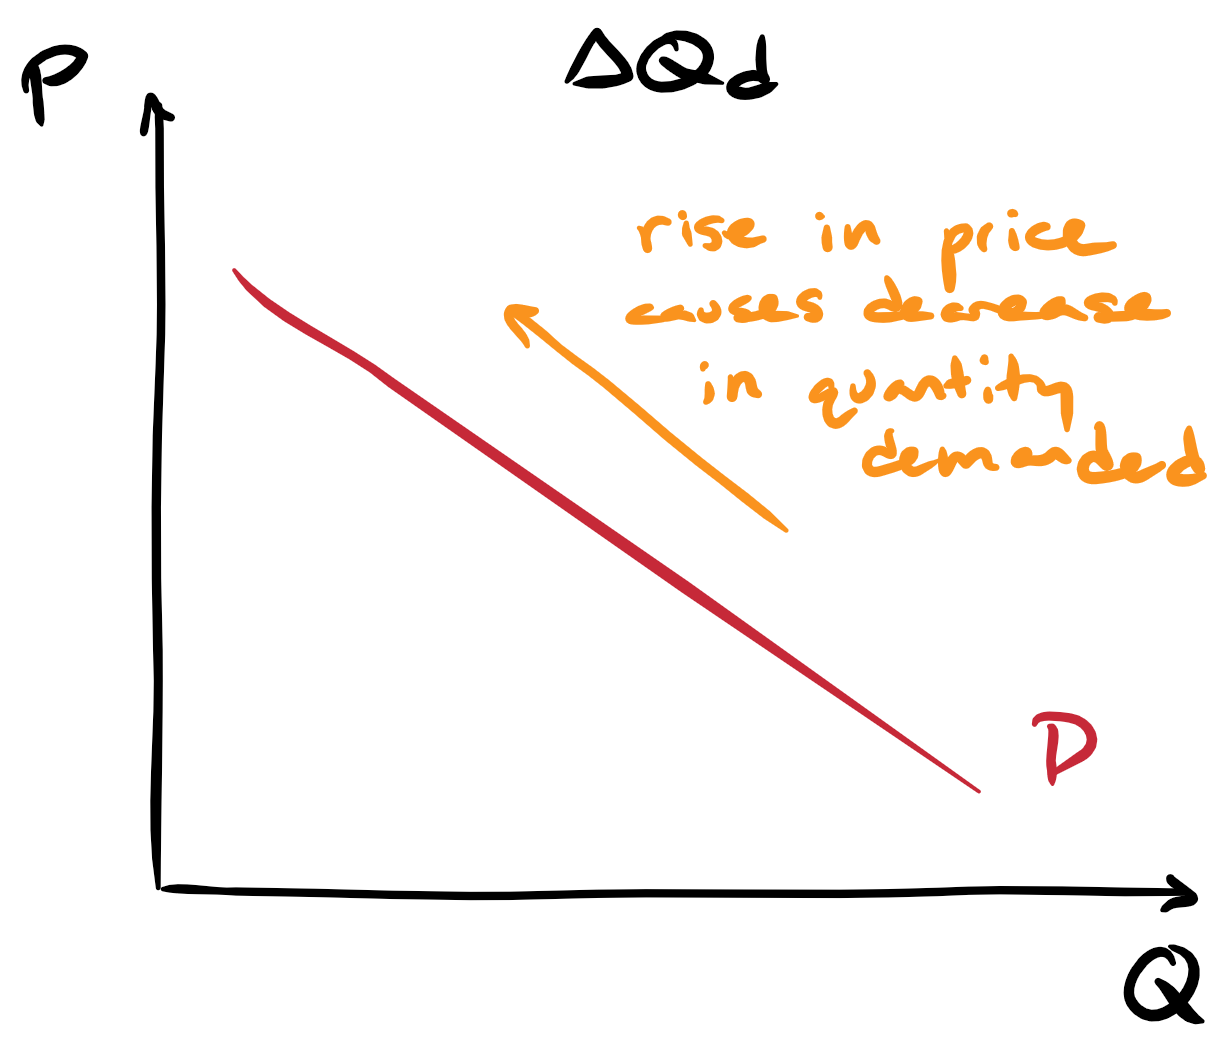
\includegraphics[width=60mm]{demand_supply_demand_pricechange1.png}
\caption{Change in Price on Demand Curve}
\end{figure}

Changes in price or quantity demand move the position up and down along the curve.

\subsubsection{Factors Influencing Quantity Demand}

But if we want to directly relate $P$ and $Q_d$ we have to hold all other factors constant, ie. ceteris paribus. The other factors influencing $Q_d$ that we'll assume are equal are \textbf{Income, Tastes, Advertising, Expectations,} and the \textbf{Price of \gls{Related Goods}}.

With normal goods, the more Income you have, the more you'll want to buy. With \gls{inferior goods}, like Kraft Dinner, typically the more money you have the less you'll want to buy. 

Expectations can delay quantity demand, but don't typically remove it. Expectations accounts for anticipating or attempting to predict the future, like gas prices going down or buying something to re-sell. 

There are two kinds of related goods: \gls{Complement goods}, goods that increase the demand for each other. For example, buying a baseball bat increases the demand for baseballs. And \gls{Substitute goods}, goods that reduce the demand for each other. For example, if you buy a coke, you're less likely to want a pepsi. 

Inversely, if baseball prices go up, your demand for baseballs goes down so your demand for baseball bats goes down. If the coke prices go up, your demand for coke goes down, so your demand for pepsi goes up.

\subsubsection{Demand Curve, $D$}

When economists talk about \gls{demand}, they aren't talking about the particular quantity being demanded at that point. They are talking about the shape of the $P$ and $Q_d$ curve - the nature of the entire relationship between the price and the quantity demand. $Q_d$ is a number, $D$ is a function of which $Q_d$ is a variable. 

These curves are always drawn assuming that all other factors other than price that influence quantity demand are held constant.

\subsubsection{Shifts of Demand Curve}

As stated above, changes in price or quantity demand move the position up and down along the curve. However, changes in the other factors (the ceteris paribus variables) doesn't move a point along the curve, it moves the position or shape of the entire curve. 

\begin{figure}[ht!]
\centering
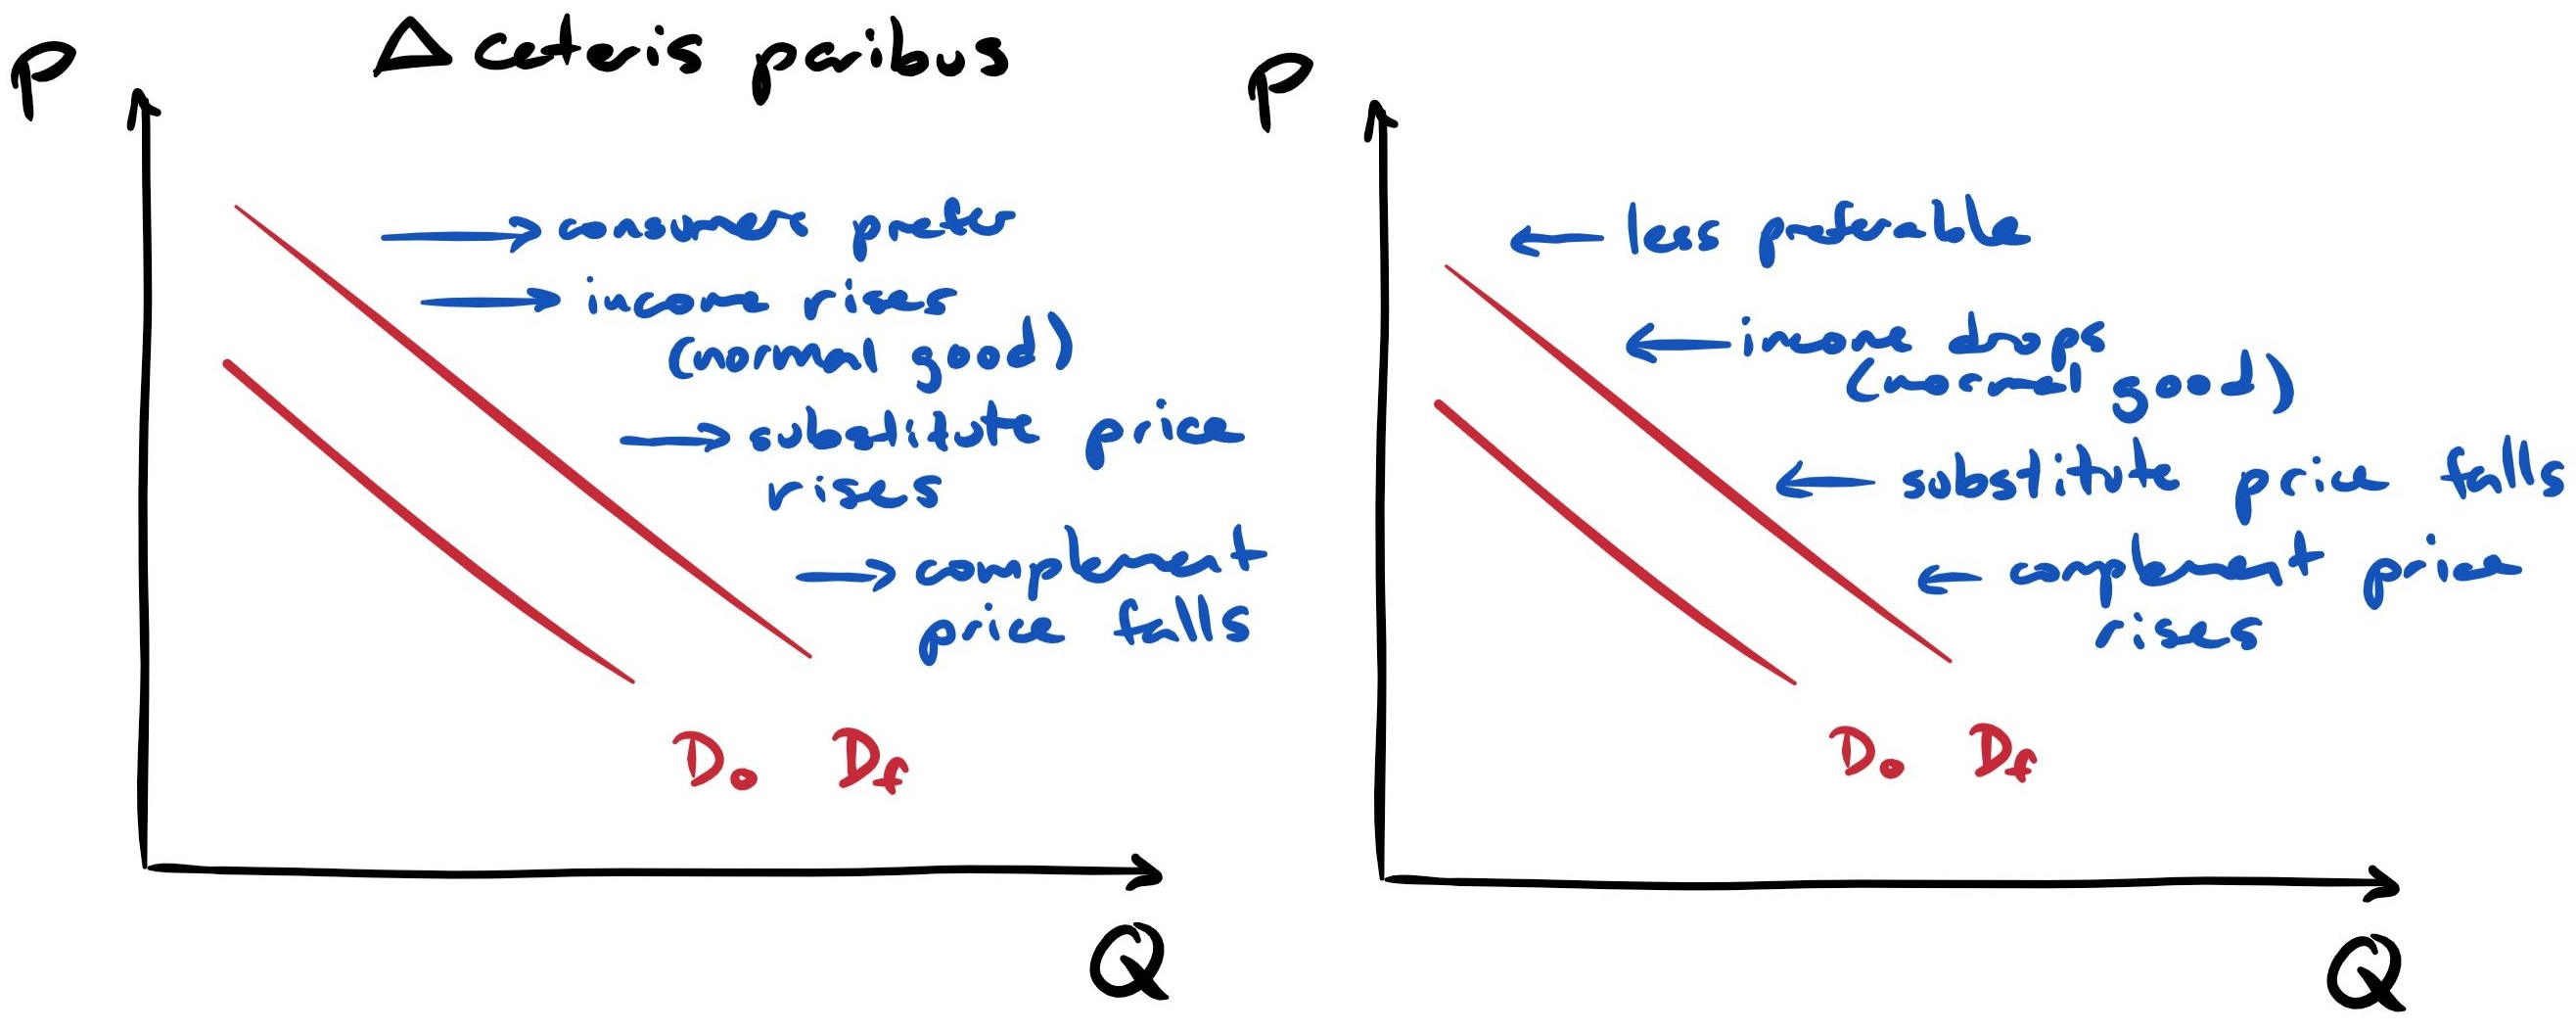
\includegraphics[width=130mm]{qd-shifts.jpg}
\caption{Shifts in the Demand Curve}
\end{figure}

Note that changes in the demand curve with the price constant results in changes in quantity demanded. 

\begin{table}[ht]
  \centering
  \caption{Causes of Shift in Demand Curve}
  \begin{tabular}{
  		>{}m{1in} 
  		>{}m{1in} 
  		>{}m{1.1in}
  		>{}m{0.8in}  		  		
  		}
    \toprule
    \textbf{Variable} & \textbf{Qualifier} & \textbf{Change} & \textbf{Effect} \\ 
    \midrule
	Income & Normal Good & Increases & Shifts Right \\
	       & Inferior Good & Increases & Shifts Left  \\
	\midrule
	Tastes &  & Consumers Prefer & Shifts Right \\
	\midrule
	Related Goods & Complement & Price Increases & Shifts Left \\
	              & Substitute & Price Increases & Shifts Right \\
	\midrule
	Expectations &  & Prices Increase & Shifts Right\\		
	\midrule
	Population &  & Rises & Shifts Right\\		
	\bottomrule

  \end{tabular}
\end{table}


\subsection{Supply}

This section is largely the inverse of the section on demand.

\subsubsection{Quantity Supply, $Q_s$}

Quantity supply is the amount of a good or service that producers want to sell \textit{per time period}. Quantity supplied is of course influenced by the price it can be sold at, but it is also affected by variables such as \textbf{price of the inputs, technology, government taxes or subsidies, prices of related goods,} and \textbf{number of suppliers}. As before, we typically hold these variables constant and focus on the product price.

When the cost to produce a product is constant and the price of a product decreases, the benefit in selling it decreases, so the opportunity cost increases and the incentive to sell it falls. Basically, there is a direct relationship between price and quantity supplied - when the price is higher the quantity supplied is higher, when the price is lower the quantity supplied is lower. 

\begin{table}[ht]
  \centering
  \caption{Causes of Shift in Supply Curve}
  \begin{tabular}{
  		>{}m{1in} 
  		>{}m{1in} 
  		>{}m{1.1in}
  		>{}m{0.8in}  		  		
  		}
    \toprule
    \textbf{Variable} & \textbf{Qualifier} & \textbf{Change} & \textbf{Effect} \\ 
    \midrule
	Input Prices &  & Increases & Shifts Left \\
	\midrule
	Technology &  & Increases & Shifts Right \\
	\midrule
		Government  & Taxes & Increase & Shifts Left \\
	\midrule
	 & Subsidies & Increase & Shifts Right \\
	 \midrule
	Related Goods & Complement & Price Increases & Shifts Left \\
	              & Substitute & Price Increases & Shifts Right \\
	\midrule
	Expectations &  & Prices Increase & Shifts Right\\		
	\midrule
	Number of Suppliers &  & Rises & Shifts Right\\		
	\bottomrule

  \end{tabular}
\end{table}

Most of these examples are simply about varying the price of cost to produce. The theme is \textbf{when costs increase, quantity supplied decreases}.

\subsection{Determination of Price}

\subsubsection{Market Equilibrium}

This sections covers how you can make both the consumer and producer happy. The quantity exchanged, $Q_e$, is how much of the good is actually purchased by the consumer from the producer. It is defined at intersection of the demand curve and the supply curve, when $Q_d = Q_s = Q_e$. At this point, the system is said to be in equilibrium. Thus the price corresponding to the $Q_e$ is the \gls{equilibrium price}, $P_e$.


\begin{figure}[ht!]
\centering
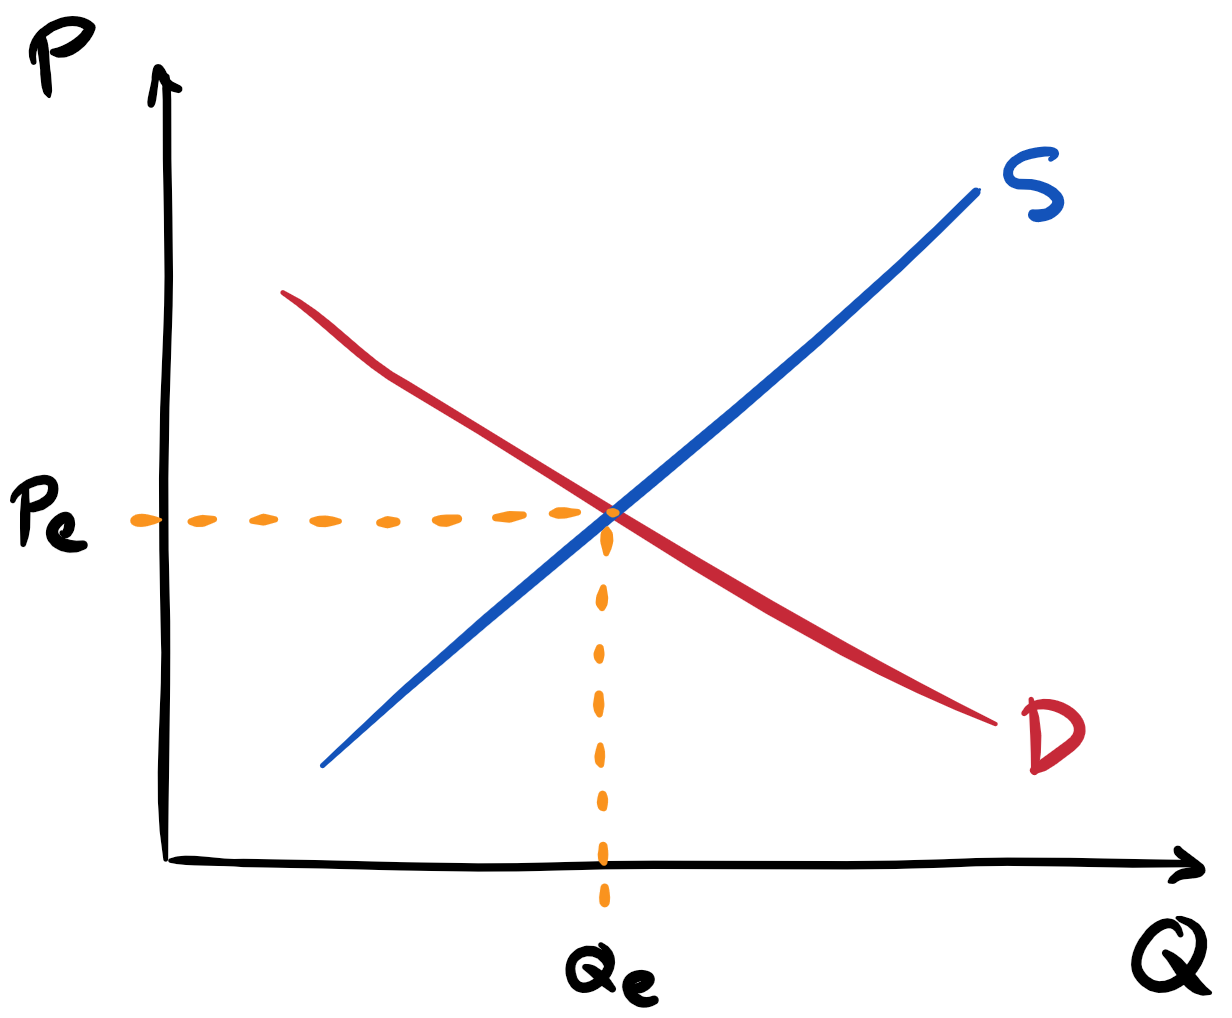
\includegraphics[width=60mm]{demand-and-supply-equilbrium.png}
\caption{Demand and Supply Equilibrium}
\end{figure}

Above the equilibrium point, $Q_s > Q_d$, so there is said to be an excess supply. Below the equilibrium point there is excess demand. An apt definition for equilibrium is that the system is happy where it is and doesn't want to move. This system is also stable, in that it is self-correcting. 

Recall our previous two findings, 1) when the price rises, the quantity demanded falls, 2) when the price falls, the quantity supplied falls. When the price or quantity demand changes, these two principles act as forces to stabilize the system. For instance in the quantity supply rises above quantity demanded, the producer will have excess inventory, which pressures the producer to reduce price. If the quantity demanded rises above the quantity supplied there will be a shortage, which incentivizes the producer to increase price. 


\begin{table}[ht]
  \centering
  \caption{Effect of Changing Quantities on Price}
  \begin{tabular}{
  		>{}m{0.8in} 
  		>{}m{0.9in} 
  		>{}m{1.2in}
  		}
    \toprule
    \textbf{Price} & \textbf{$Q_s$ and $Q_d$} & \textbf{Effect on Price} \\ 
    \midrule
	$P_e$ & $Q_s = Q_d$ & Remain constant  \\
	$> P_e$ & $Q_s > Q_d$ & Push lower  to $P_e$ \\
	$< P_e$ & $Q_s < Q_d$ & Push higher to $P_e$  \\
	\bottomrule

  \end{tabular}
\end{table}

Due to these pressures, the market price will always tend towards the equilibrium price. Prices at which $Q_e != Q_d$ are said to be disequilibrium prices because the market is in a state of disequilibrium the market price is changing.  

\subsubsection{Shifts in Market Equilibrium}

In the above section we focused on movement along the curves due to changes in quantity supplied and quantity demanded. As before, changes in the other factors such as tastes, income, taxation, technology, or prices of related goods, cause movement of the demand or supply curves themselves. 

\begin{figure}[ht!]
\centering
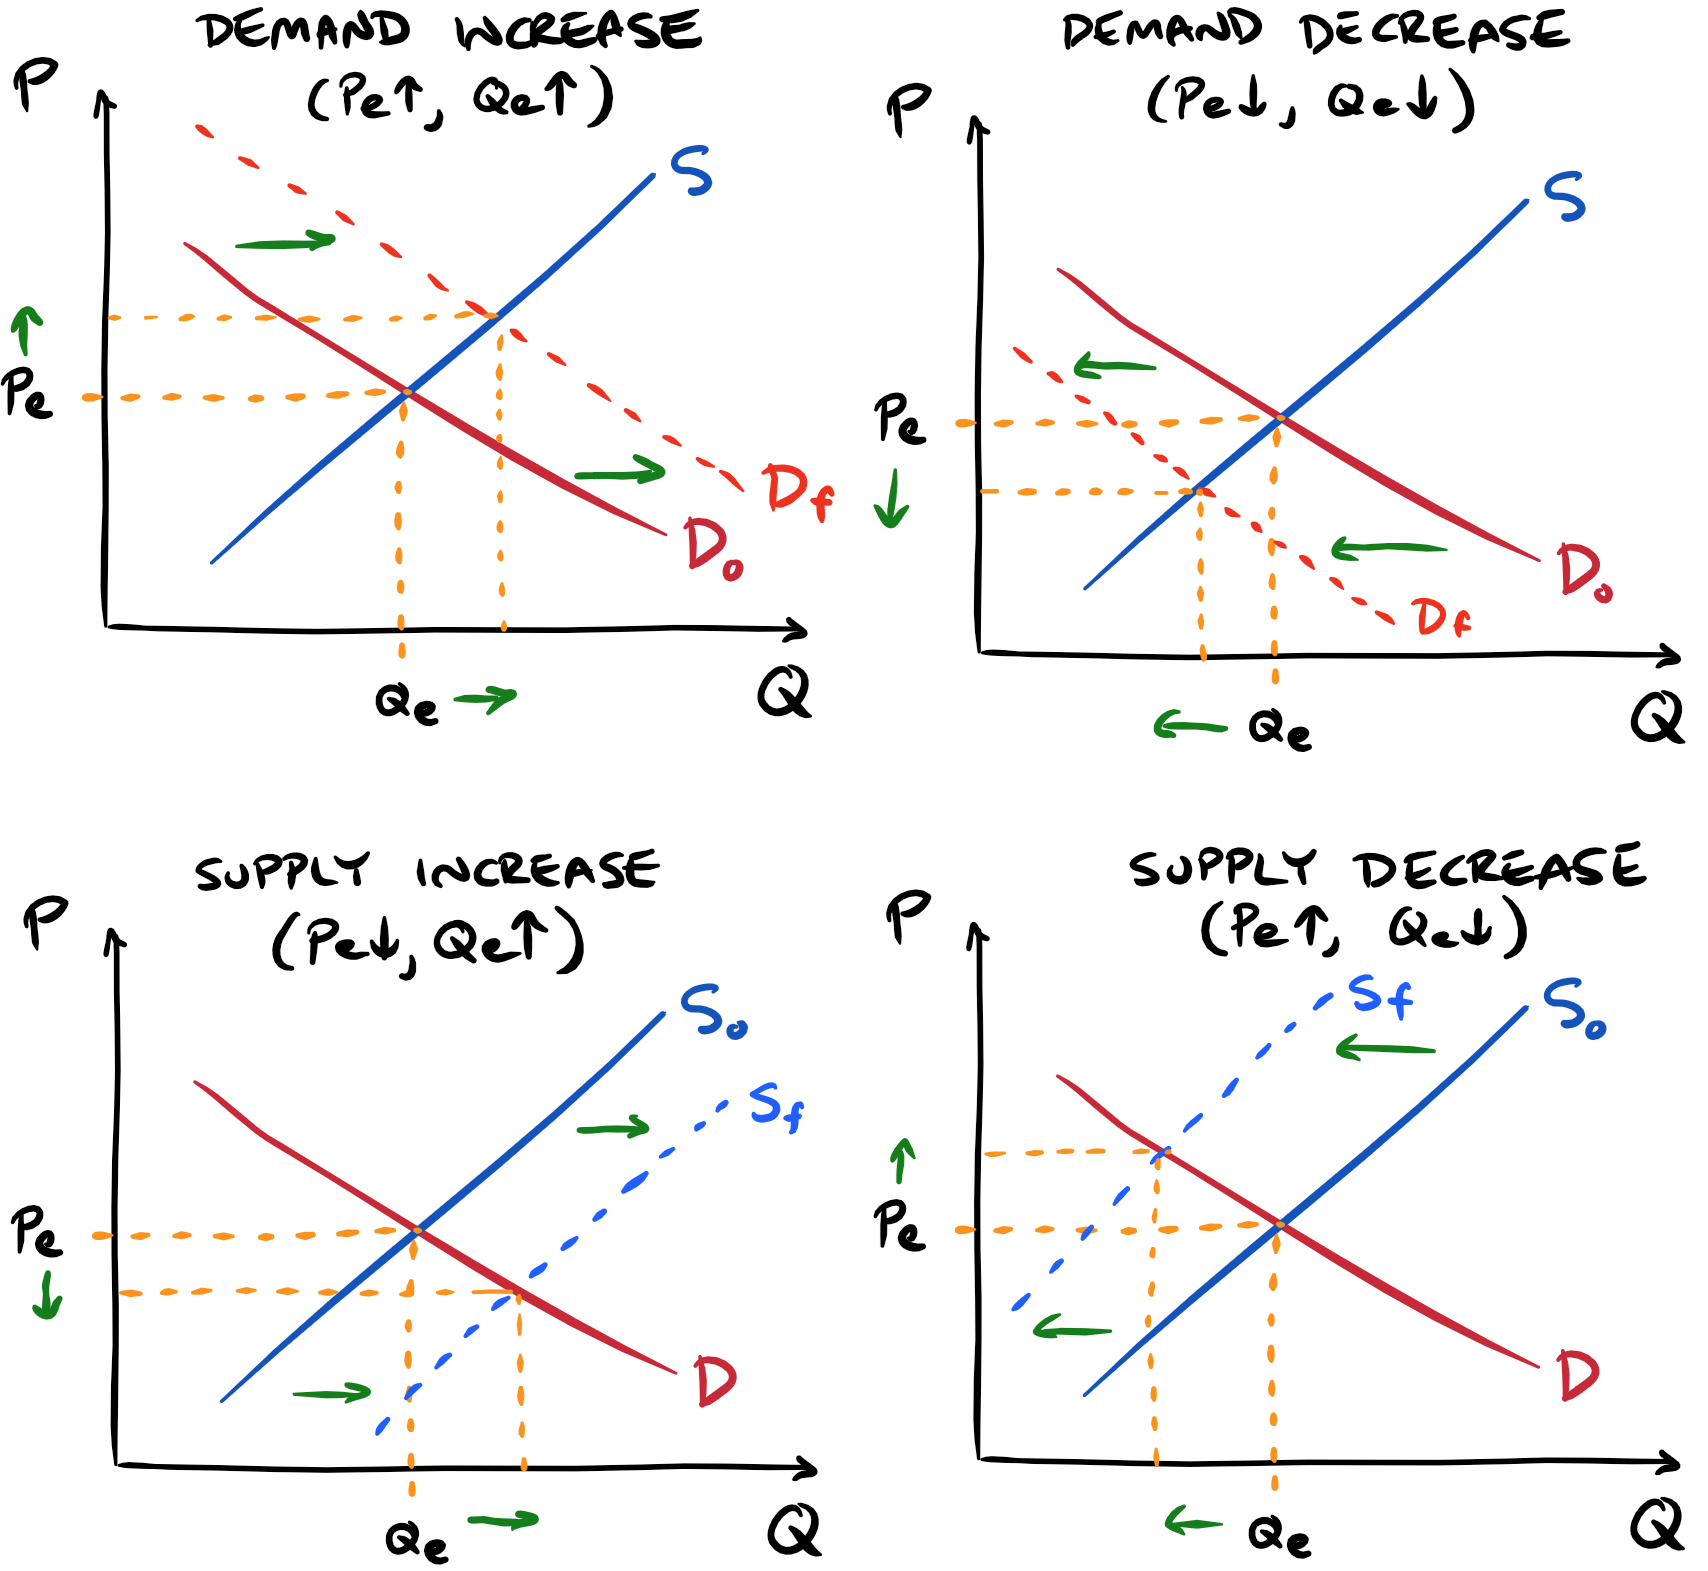
\includegraphics[width=120mm]{tax-incidence-supply-demand-diagrams.png}
\caption{Shifts in Equilibrium}
\end{figure}


When these curves shift it moves the position of the intersection, changing $P_e$ and $Q_e$. An increase in demand moves the demand curve to the right, which rises the quantity exchanges and the equilibrium price. An increase in supply moves the supply curve to the right, which rises the quantity exchanged and decreases the equilibrium price.

\subsubsection{Relative Prices and Inflation}

Absolute prices are simply the money it takes to buy something. Relative prices however are the ratio of two absolute prices - the price in terms of another good. 

If the price of carrots increases but the price of other vegetables stays constant, the relative price of carrots has increased. In this situation we expect people to just buy potatoes and parsnips instead.  However, if the absolute price of all root vegetables increases, the relative price of carrots is constant. In this situation, we don't expect to see people substituting parsnips for carrots. 

In a world of inflation, when we talk about changing prices we must talk about changing \textit{relative} prices.

\section{Elasticity, $ \eta $}

The shape of the demand and supply curve of a product shows how sensitive it is to changing price or quantity. This sensitivity as called elasticity. 

\gls{Inelastic} products are insensitive to changes. For example, if the price of cigarettes increases, most cigarette consumers will still buy cigarettes because they're addicted. So cigarettes are inelastic.  

\gls{Elastic} products are elastic because when the price increases, the $Q_d$ substantially decreases because people will just buy something else.

\subsection{Price Elasticity of Demand}

The price elasticity of demand is defined as the relative change in quantity over the relative change in price. Relative change is defined as $\frac{\Delta X}{X} = \frac{X_{final} - X_{initial}}{X_{average}}$.

$$ \eta = \frac{\Delta Q / Q}{\Delta P / P} = \frac{\Delta Q}{\Delta P} \frac{P}{Q} $$

For elastic products,  $\eta > 1$, and for inelastic products, $\eta < 1$. When $\eta = 0$, change in price has \textit{no change} in $Q_d$, thus has a vertical demand curve. When $\eta = \infty$ there is a horizontal demand curve, meaning any change in price causes massive change in $Q_d$.


\begin{figure}[ht!]
\centering
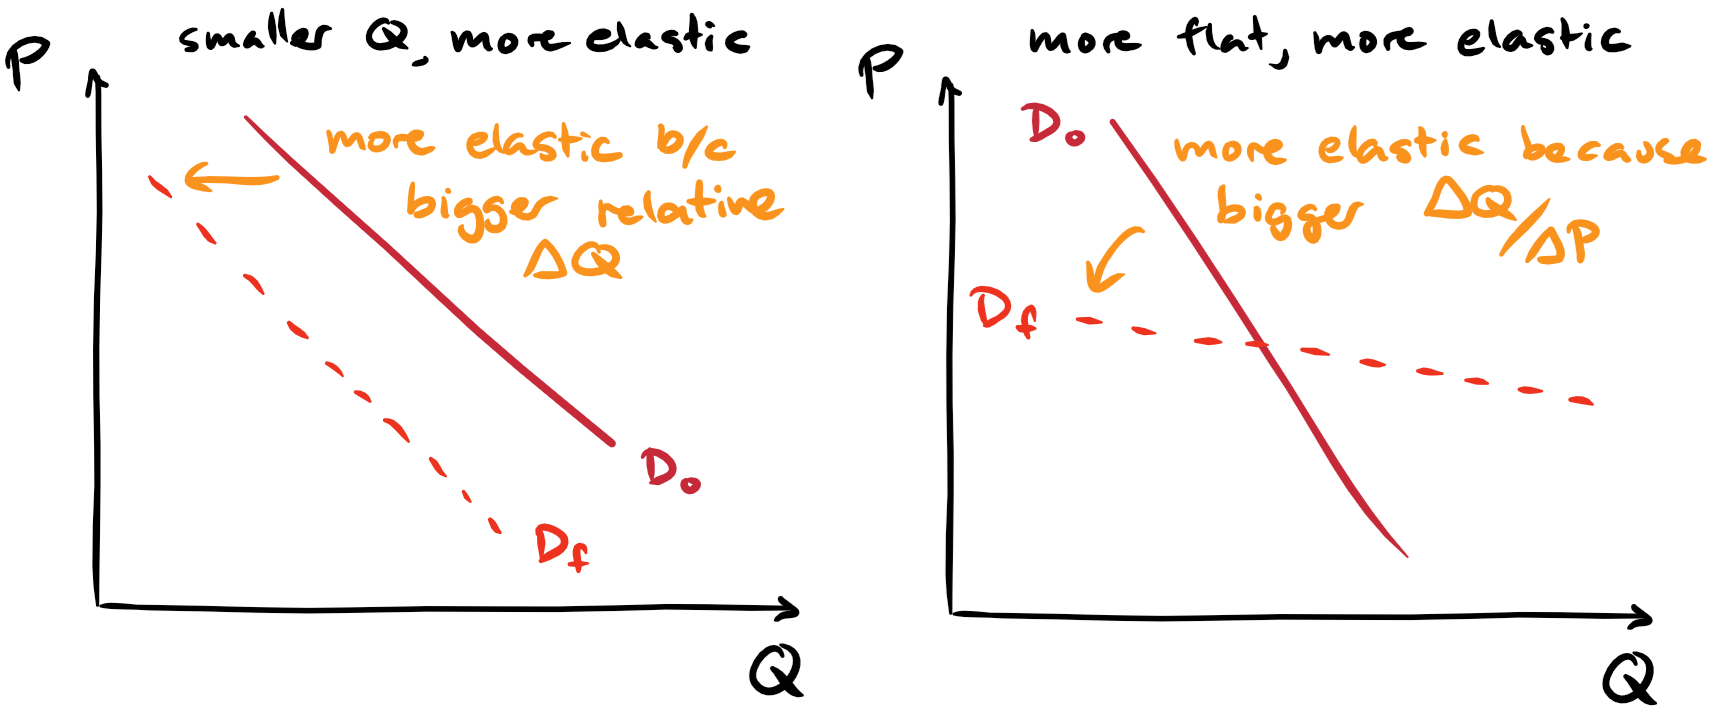
\includegraphics[width=130mm]{elasticity.PNG}
\caption{Effect of Elasticity on the Demand Curve}
\end{figure}


Elasticity can also be seen by the shape and position of the demand curve. The higher the absolute value of $Q$, the less significant $\frac{\Delta Q}{Q}$ is, therefore the smaller the elasticity. So given parallel demand curves, the curve further to the right has the lower elasticity. 

\begin{figure}[ht!]
\centering
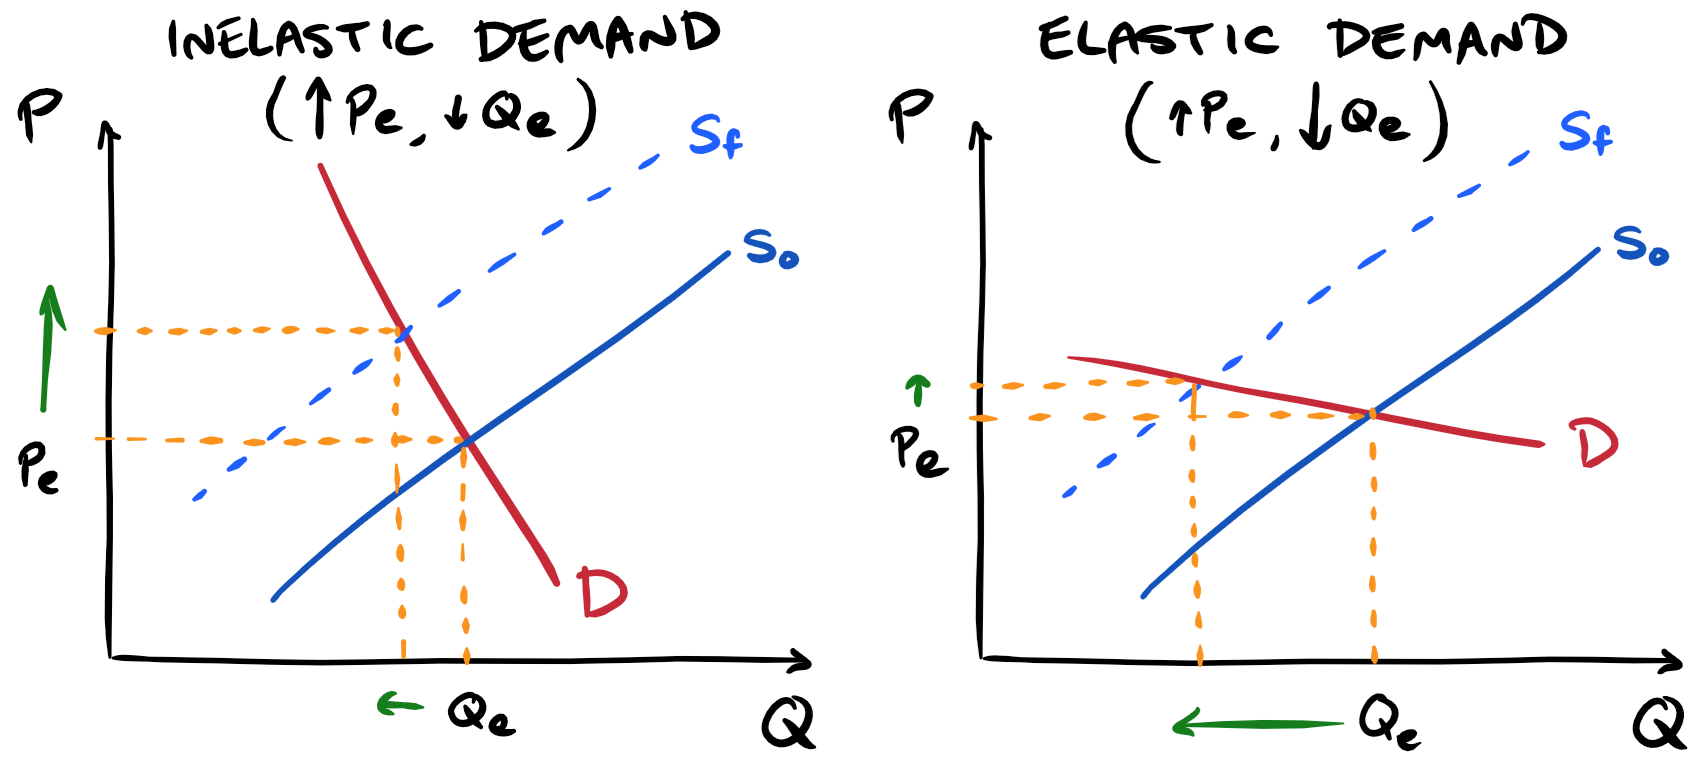
\includegraphics[width=130mm]{elastic-inelastic-time-diagrams.png}
\caption{Effect of Price Change with Different Elasticities}
\end{figure}

The other way to see elasticity is by the slope of the demand curve. The flatter it is, the more elastic it is. As seen in Figure 6, with the steeper curve, a small change in equilibrium price causes a larger change in equilibrium quantity.



\begin{table}[ht]
  \centering
  \caption{Types of Elasticity}
  \begin{tabular}{
  		>{\centering}m{0.3in} 
  		>{}m{0.8in} 
  		>{}m{1.1in}
  		>{}m{1.6in}  		  		
  		}
    \toprule
    \textbf{$\eta$} & \textbf{Shape} & \textbf{Term} & \textbf{Description} \\ 
    \midrule
	$0$ & Vertical 	& Perfectly inelastic 	& $Q_d$ does not change with $P$ \\
	$<1$ & Steep 		& Inelastic 			& $\Delta Q < \Delta P$ \\
	$=1$ & Hyperbola	& Unitary elastic		& $\Delta Q = \Delta P$ \\
	$>1$ & Flat 		& Elastic 				& $\Delta Q > \Delta P$ \\
	$\infty$ & Horizontal & Perfectly elastic & $P$ does not change with $Q_d$\\
	\bottomrule

  \end{tabular}
\end{table}

Note that when elasticity is constant, the demand curve is hyperbolic. So when the demand curve is linear, elasticity is different along all points of the slope and falls as price decreases. 



\subsubsection{Factors Determining Elasticity of Demand}

Elasticity of demand is mostly effected by the \textbf{availability of substitutes}. Products that close substitutes have larger elasticity because people will switch to alternatives. 


The elasticity also depends on the \textbf{time period of consideration}. Even if a product is inelastic because it doesn't have substitutes, over time there will be a gradual increase in substitutes and therefore over time products become more elastic. Graphically, this is seen as a rotation of the demand curve.


Finally, elasticity also depends on \textbf{budget-share}. More expensive items tend to have higher elasticity than cheaper items, for examples cars are more elastic than apples. 



\subsubsection{Effect on Revenue}

Total revenue is the amount of product sold times the price, $R = P_e Q_e$. So revenue is at a maximum when price and quantity are balanced, in other words at unit elasticity, $\eta=1$.

\begin{figure}[ht!]
\centering
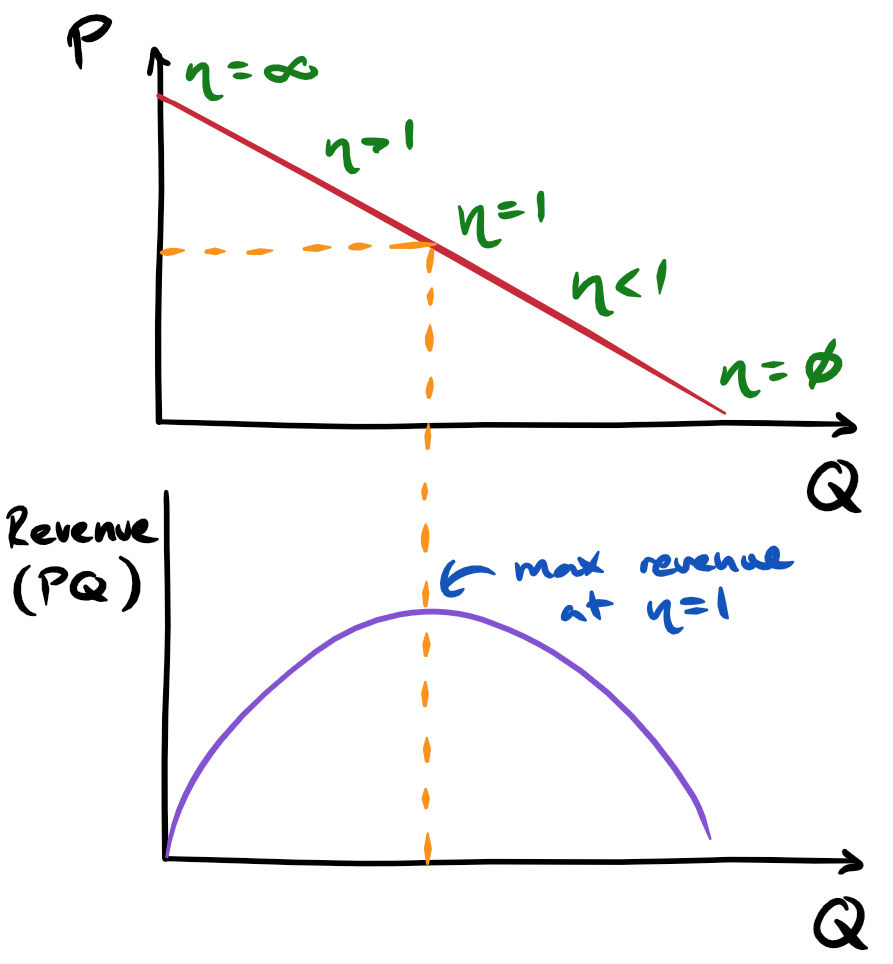
\includegraphics[width=80mm]{Demand_Elacticity.png}
\caption{Total Revenue with Elasticity}
\end{figure}


\subsection{Price Elasticity of Supply}

For supply it is mostly the same, except you look at $Q_s$ instead of $Q_d$. The main difference is what determines the elasticity. In the case of elasticity of supply, instead of availability of substitutes of outputs it's availability of substitutes of inputs (capital, land, labour, technology, etc). 

Elasticity of supply depends on how easy it is for a supplier to convert outputs. For example, if the price of wheat rises then a oats producer could cheaply convert to the production of wheat, thus there is a high supply elasticity. Whereas a cranberry producer could not cheaply convert to the production of wheat, therefore it is an inelastic supply. 

Similarly with demand, elasticity of supply increases over time. 

\subsection{Income Elasticity of Demand}

Income elasticity of demand is relative changed in quantity demand over relative change in income, $\eta = \frac{\Delta Q / Q}{\Delta Y / Y}$. 

\subsubsection{Goods}

With luxury/normal goods, as income, $Y$, increases the $Q_d$ increases so there is a positive and substantial elasticity. When people can't afford things, they won't buy them (ex. movie tickets). With necessities, like toilet paper, income doesn't have much of an effect on quantity - people don't win the lottery then decide to buy more toilet paper. Finally, with inferior goods like Kraft Dinner, there  is actually a negative elasticity because as income increases, quantity demanded decreases. 

\subsection{Tax Incidence}

An interesting quality of elasticity is it defines who picks up the tab when government impose additional taxes on a product (excise taxes). Tax incidence is the percentage of tax paid by the consumer. 

\begin{figure}[ht!]
\centering
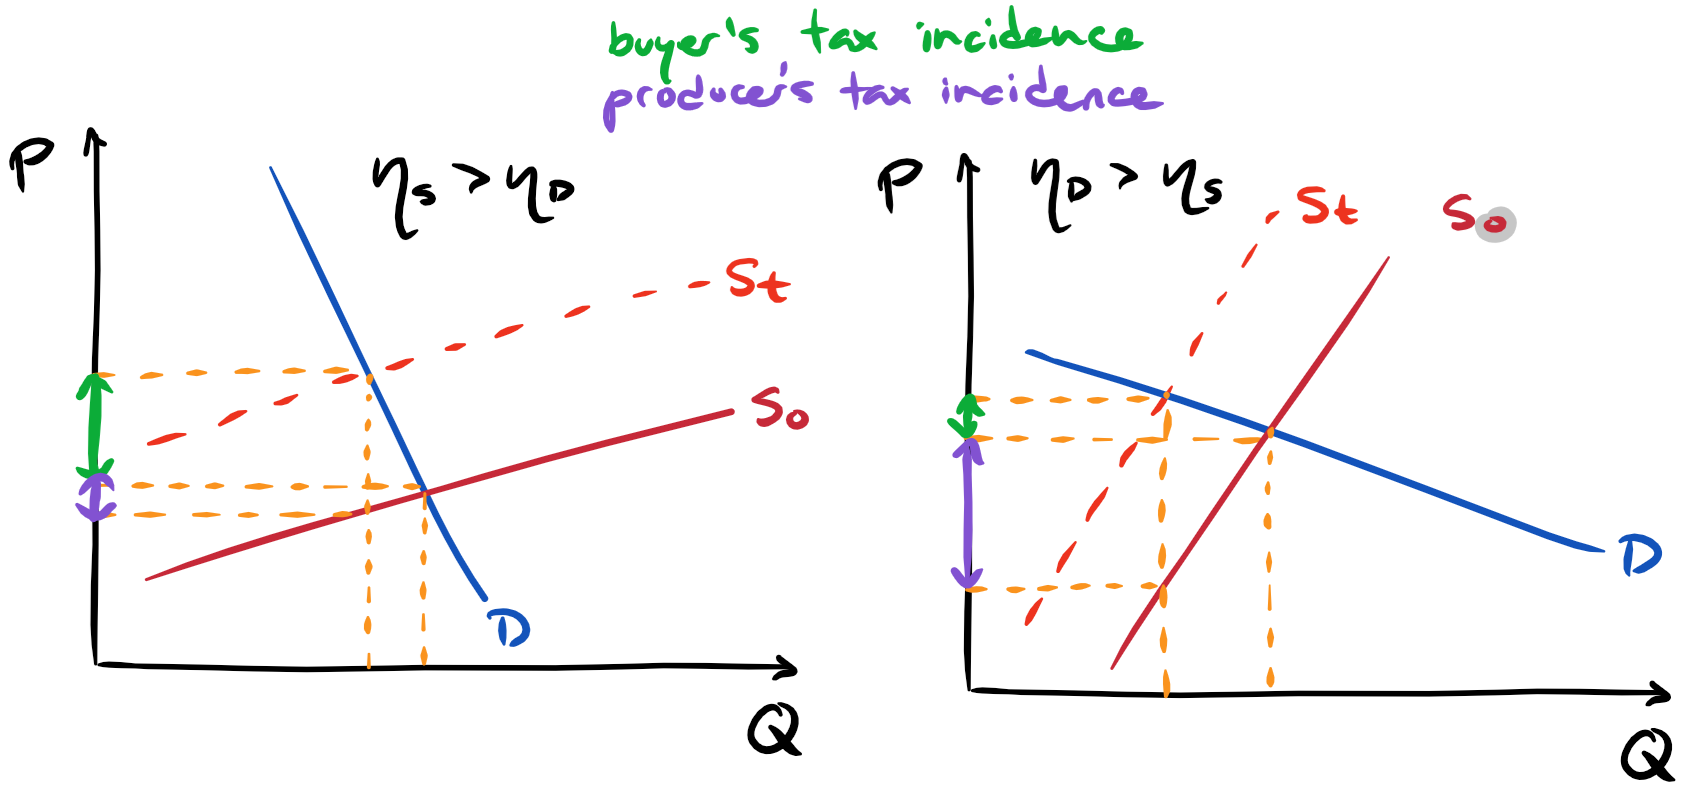
\includegraphics[width=130mm]{Shifts-in-Demand-Supply-Curves.png}
\caption{Tax Incidence of Elasticities}
\end{figure}


When demand is more elastic than supply, most of the tax is paid by the producer. When supply is more elastic than demand, most of the tax cost is paid by the consumer. 

This is why extra taxes can be placed primarily on goods like alcohol and cigarettes that have inelastic demands. 

\subsection{Cross-Elasticity}

Cross-elasticity describes when the change in price of one good affects the quantity demanded of another good, $\eta = \frac{\Delta Q_x / Q_x}{\Delta P_y / P_y}$.

A change in price of good $Y$ can cause the demand curve of good $X$ to shift. If the products are substitutes, like coke and pepsi, an increase in the price of coke increases the $Q_d$ of pepsi. If the products are complements, like a baseball and a baseball bat, if the price of the baseball bat increases, the $Q_d$ of baseballs decreases. 

Given cross-elasticity, which ranges between negative and positive infinity, one can determine whether two products are complimentary goods or competing goods. Complimentary goods have a negative cross elasticity, and substitute goods have a positive cross elasticity. 

\section{Markets in Action}

The economy is a complex system of interconnecting markets and no market is isolated from the economy's other markets. 

A change in one market will lead to a change in another market, which in turn will lead to changes in the initial market. This cycle is called \gls{feedback}. 

We will focus on the analysis of single markets in isolation and ignore any effects of feedback. This is called \gls{partial-equilibrium}. \gls{General-equilibrium} is the analysis of all markets simultaneously, sometimes called dynamic analysis because in addition to $P$ and $Q$, another variable, time, is included. 

\subsection{Government-Controlled Prices}

\subsubsection{Disequilibrium Prices}

When the government implements price control policies, they are trying to hold the price at some disequilibrium value. A disequilibrium price is any price other than the equilibrium price. At a disequilibrium price, the quantity exchanged is the lesser of the quantity demanded and supplied.


\begin{table}[ht]
  \centering
  \caption{Causes of Shift in Demand Curve}
  \begin{tabular}{
  		>{}m{1in} 
  		>{}m{1in} 
  		>{}m{1.1in}
  		}
    \toprule
    \textbf{Price} & \textbf{Quantity} & \textbf{Description} \\ 
    \midrule
	$> P_e$ & $Q_d>Q_s$ & Shortage \\
	$= P_e$ & $Q_d=Q_s$ & Eveyone's happy \\
	$< P_e$ & $Q_d<Q_s$ & Glut \\

	\bottomrule

  \end{tabular}
\end{table}



\subsubsection{Price Floors}

A price floor is a set minimum price that something must be bought at. Legislated minimum wage is a price floor, because people cannot sell their labour for less than the set wage. If the price floor is below the below the equilibrium price, the price floor has no effect. However, when the price floor is above the equilibrium price, it will lead to an excess supply. 

In the case of the labour market, this means unemployment. Typically price floors are set on agricultural products, with the excess supply being bought up by the government and stockpiled. 

\subsubsection{Price Ceilings}

A price ceiling is the maximum price at which a product can be sold. When the price ceiling is above the equilibrium price, this has no effect, but when the price ceiling is below the equilibrium price, quantity demanded exceeds the quantity supplied, leading to shortages. Examples of price ceilings are affordable housing, tuition freezes, gas ceilings, etc. 


\begin{figure}[ht!]
\centering
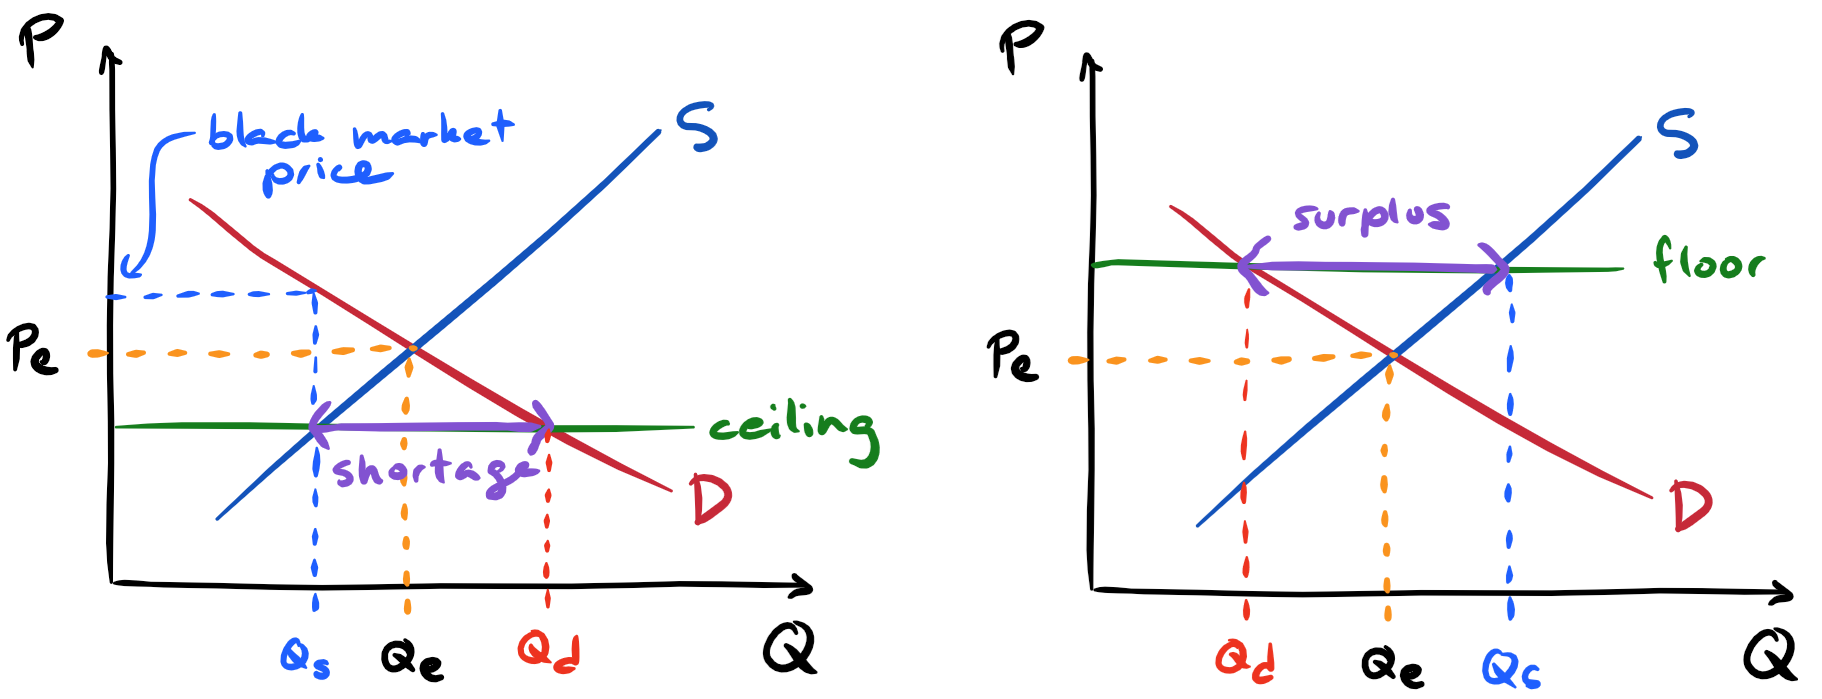
\includegraphics[width=130mm]{black-market.png}
\caption{Price Controls and Black Market}
\end{figure}


In the case of shortages due to price ceilings, people typically manage allocation of resources in a few different ways. \textbf{First-come, first-serve} is very common, this causes people to wait in long lines to try to get the commodity before it runs out. Another method of allocation is \textbf{sellers' preference}. When goods are in short supply, sellers can be confident that they will clear there inventory and thus may choose who to sell to, for example family and friends. Seen in many countries during the Second World War is \textbf{rationing}. In the case of rationing, the government prints only enough ration coupons to match the quantity supplied at the price ceiling and then distributes the coupons evenly. This means would-be purchasers need the money and the coupons.


However, all of these methods of allocation are susceptible to \gls{black markets}. Black markets are markets that violate government price control. First-come, first-serve is prone to scalpers, who buy up inventory then sell it at monopoly profits (the price corresponding to the $Q_S$ on the demand curve. And even rationing causes people to sell their rationing coupons for a higher price. 

\subsubsection{Market Efficiency}

Minimum wage is a contentious issue because it benefits those who currently are employed, but harms firms and future job-seekers. \gls{Market efficiency} is how the harm to one group is weighed against the harm to another group to determine what benefits society as a whole.

To quantify what determines the overall benefit to society, it is helpful to visualize the demand curve as "value" and the supply curve as "cost". Price of demand shows the value consumers place on the item. The price on the supply curve shows the lowest price firms will accept for that item. This price reflects the cost of production to the firm. 


\begin{figure}[ht!]
\centering
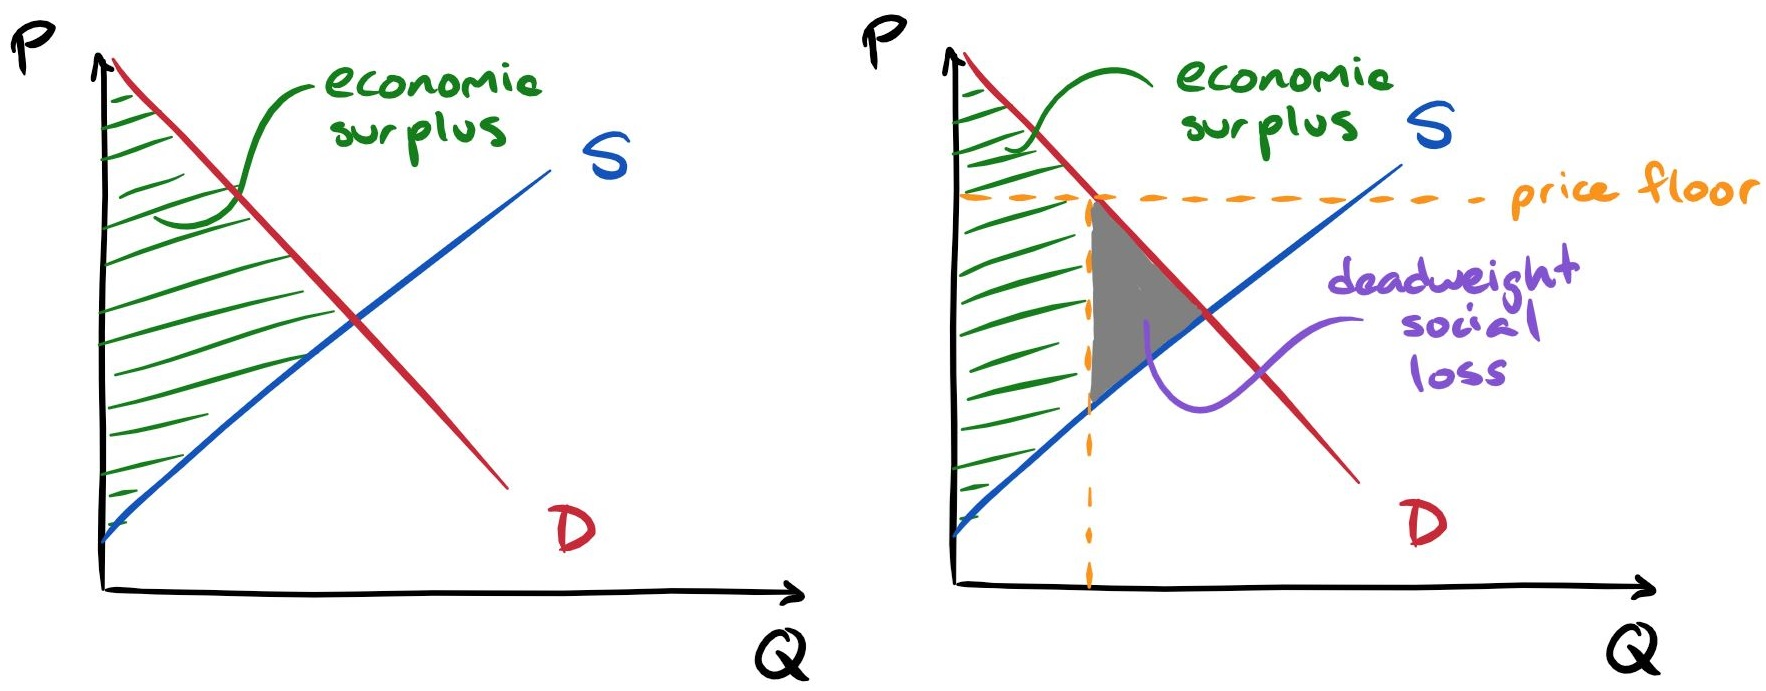
\includegraphics[width=130mm]{dwsl.jpg}
\caption{Market Efficiency and DWSL}
\end{figure}


To the right of the equilibrium point, the "value" exceeds the "cost", resulting in economic surplus. This economic surplus is the net value gained by society as a whole. For example, if the value consumers place on Q=10 pizzas is P=\$100, and the value supplier place on Q=10 pizzas and P=\$20, then the producers have taken something of lower value and turned it into something of higher value. This is the overall benefit to society.

The value is all of the area underneath the demand curve and the cost is the area underneath the supply curve, from $Q$=0 to $Q_e$. The economic surplus is the value-cost, so the area between the curves. This area is maximized when $Q=Q_e$. To the right of $Q_e$ you begin to have negative economic surplus because the cost to suppliers exceeds the value to consumers. 

\subsubsection{Effect of Price Controls}

When the government imposes price controls, this reduces the economic surplus area and creates market inefficiency because the area to the left of the new $Q_e$ is unreachable. This lost economic surplus is called \gls{deadweight social loss}. 


\subsubsection{Output Quotas}

Quotas restrict the maximum quantity of output for suppliers. This forces the quantity to be below the $Q_e$, which increases the product's price. 

If the demand is inelastic, then the increase in price is larger than the decrease in quantity, which means the supplier's income rises. If the demand is elastic, then the decrease in quantity outweighs the increase in price, which means the supplier loses income. This is why quotas are usually only put on inelastic products, like dairy. 

One of the major obstacles of quotas is that it is expensive to purchase quotas so there are large barriers for new producers wanting to enter the industry.

\section{Consumer Behaviour}

This section discusses how consumers behave in an effort to maximize their happiness. Consumers care both about the price of the goods and the satisfaction they get from the goods.

\subsection{Marginal Utility and Consumer Choice}

Utility cannot be measured directly, but it is still a useful concept. Total utility is the total satisfaction the consumer gets from consuming a good. Marginal utility on the otherhand is the satisfaction that could be obtained from consuming one additional unit of that good.

\subsubsection{Diminishing Marginal Utility}

For each successive unit of a good consumed, the utility the consumer gets from the good diminishes as the total consumption increases. Basically, the more of something you consume, the less happiness you get from it.

This assumes you hold constant all other variables.

\begin{figure}[ht!]
\centering
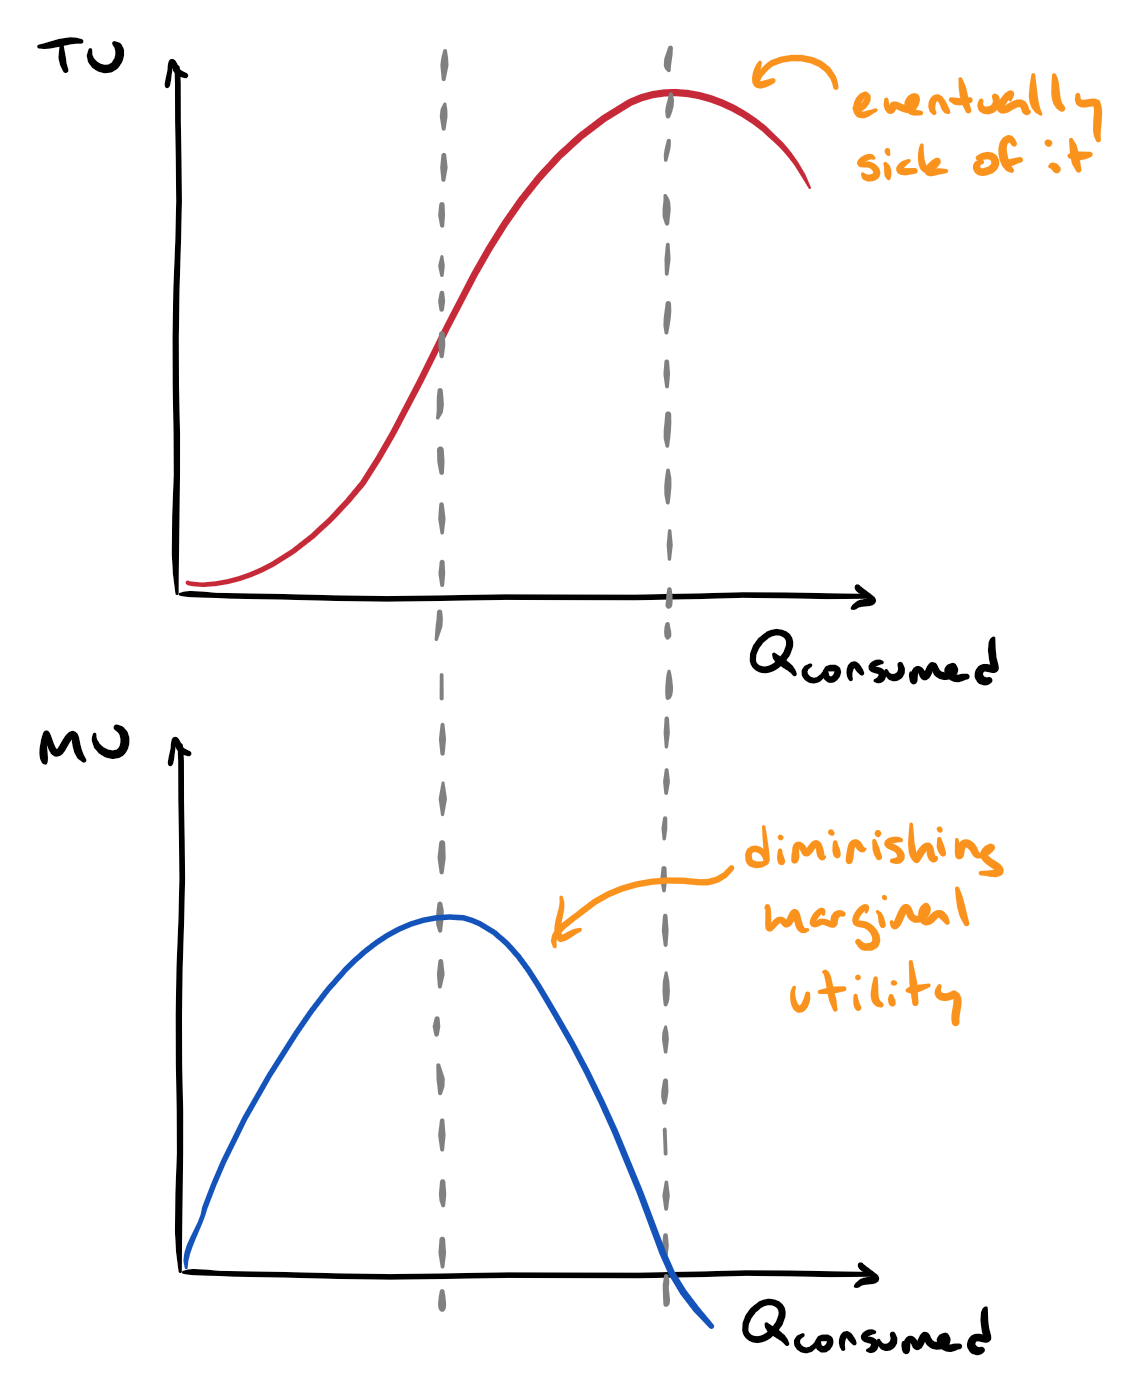
\includegraphics[width=70mm]{diminishing-total-utility.png}
\caption{Marginal/Total Utility}
\end{figure}

As you can see from the graphs, the marginal utility is the slope (derivative) of the total utility. Initially, the curve is rising and accelerating, then the curve is rising and deccelerating, then the curve is dropping and deccelerating. 

\subsubsection{Maximizing Utility}

Let's say you have two options, beer and pizza, and need to figure out how much of each to consume to maximize your happiness. To maximize your utility, you equate the marginals. In other words, the marginal utility per dollar, $MU/P$, of pizza must equal the marginal utility per dollar of beer.

$$\frac{MU_x}{P_x} = \frac{MU_y}{P_y}$$

Notice that this means that you're not getting more utility from one product per dollar than you are another product. If the $\frac{MU_{pizza}}{P_{pizza}} >  \frac{MU_{beer}}{P_{beer}}$ because the price of beer increased, then you should start buying more pizza because it gives you more happiness per dollar than beer. But as you increase how much pizza you're consuming, by the law of diminishing marginal utility, the $MU$ you get from pizza will gradually drop, and the equation will again equalize.

We can also look at it another way, first by rearranging the equation.

$$\frac{MU_x}{MU_y} = \frac{P_x}{P_y}$$

The right side of the equation is the relative price of the goods, which you don't have any control over. The left side of the equation is the relative utilities of the goods. You can't directly control the $MU$ you get from a good, but by increasing your consumption of a good, you indirectly decrease the $MU$ of that good and vice-versa. So let's say now $\frac{MU_{pizza}}{MU_{beer}} < \frac{P_{pizza}}{P_{beer}}$ because the price of pizza increases. In order to maximize your happiness by equating the marginals, you should consume more beer so that the $MU_{beer}$ decreases. Then the equations will again stabilize. 

So this is all neat, but you might be thinking now "okay, when I'm in 7-11 and getting food and deciding what to buy, I'm not comparing my relative marginal utilities and price ratios". And you're right, but these formulas aren't an explanation of \textit{why} or \textbf{how} consumers make their decisions. Instead, what they're doing is describing the behaviour of consumers in such a way that predictions can be made. 

\subsubsection{Deriving the Consumer Demand Curve}

Before we just said the demand curve was negatively sloped and just rolled with the idea that when prices increased, consumers wanted less and when prices decreased, the consumers wanted more. Now we can actually derive this behaviour with the formula $\frac{MU_x}{MU_y} = \frac{P_x}{P_y}$. 

In this case, we're not really comparing two products though. We're comparing the product we want to make the demand curve for, let's say coffee, and the \textit{all other products}. If you're buying coffee, you're buying less of the rest of the other possible goods you could buy, and vice-versa.

When the price of coffee $P_x$, increases, in order to equalize the equation, $MU_x$ needs to be increased. The only way to increase $MU_x$ is to decrease the consumption of coffee. On the otherhand, when the price of coffee decreases, in order to stabilize the equation $MU_x$ needs to decrease, which can be accomplished by increasing consumption.

That's the same behaviour we took for granted earlier: the price of $P$ causes a decrease in $Q_d$.


\subsubsection{Market Demand Curve}

The market demand curve is found by summing the demand curves of all individual consumers. However,  note that it's a \textit{horizontal} summing of quantities, not prices. 

\begin{figure}[ht!]
\center
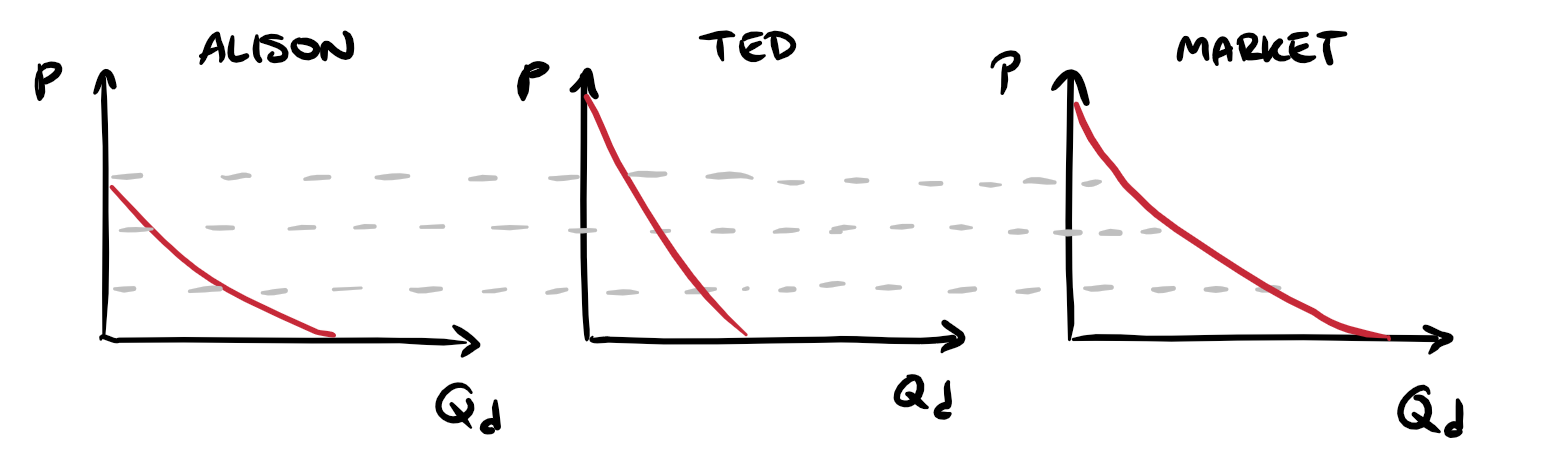
\includegraphics[width=100mm]{market-demand-curve.png}
\caption{Individual and Market Demand Curves}
\end{figure}

This just reflects the demand curves of everyone in the market. At a certain price, $P$, Alison wants 5, James wants 3, and Ted wants 7. So at the price $P$, the market wants 15.

\subsection{Income and Substitution Effects of Price Changes}

So we know that when a price decreases, the quantity demanded increases. However, there are two separate factors that make that the case. First, let's define real income/purchasing power as the quantity of goods that can be purchased with income. Note this isn't the same as income, because if the price of a good drops, your income doesn't increase. However, if the price of a good drops, now you can buy more things, so your real income does increase.

\subsubsection{Substitution Effect}

If the price of beer drops and the price of wine doesn't. It'll provide an incentive for you to stop buying wine are buy more beer, because you can still satisfy your craving to tie one, but now you can do it more cheaply.

To observe substitution effect, you have to hold real income constant. In other words, when the price of a good decreases, your income also drops so that your purchasing power is the same. When we do this, any change in $Q_d$ we see as a result in the change of relative price is due to the substitution effect.

Substitution effect is pretty much always, the same. When the price of a good goes up, people demand less. When the price of a good goes down, people demand more. 

\subsubsection{Income Effect}

When the price of beer drops, you don't need to spend as much on beer so you can buy more of everything. That is, you have more net purchasing power/real income. Recall as we discussed earlier, with a normal good, when your income increases your $Q_d$ increases. That's the same with real income. When people have more net purchasing power, they want to buy more of everything, including beer. So the income effect is what describes that contribution. 

To observe income effect, you have to hold relative price constant. In other words, ignore that you might buy more beer because you're going to substitute away for wine, and assume you're just buying more beer because you have more real income. 

\begin{figure}[ht!]
\centering
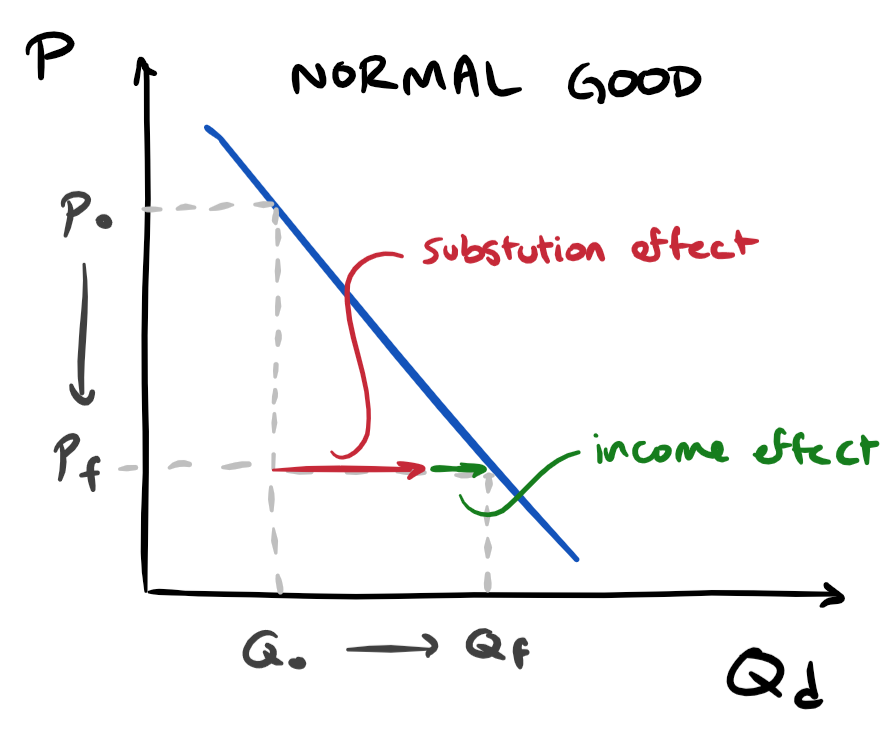
\includegraphics[width=80mm]{sub-inc-normal-good.png}
\caption{Substitution/Income Effect of Normal Good}
\end{figure}

For normal goods, the income effect works in the same direction as the substitution effect -- ie. rise in price causes drop in demand and vice-versa. However, with inferior goods, recall the income effect pushes in the opposite direction of substitution effect and they cancel eachother.


\subsubsection{Contradictions of the Demand Curve}

When we create the demand curve, we combine the substitution and income effects. This pretty much always results in a negatively sloped demand curve except in the freak case of Giffen Goods. 

Imagine you're a poor peasant and 90\% of your diet is bread, but on Sundays you'll buy yourself a nice bag of potatoes. If suddenly the price of bread rises, you won't be able to afford your delicious potatoes anymore, so instead will have to stick with buying bread instead of splurging on potatoes on Sunday. This seems to violate the negatively sloped demand curve, because as the price of the good increases, the quantity demanded of the good rises -- a positive demand curve. This is a Giffen Good.

Giffen Goods are extremely rare in the developed world, and do not exist unless 1)  the good is an inferior good, and 2) the good takes up a large proportion of the total household expenditure. In this case, the income effect is so large that it outweighs the substitution effect and the demand curve is positively sloped. 

\begin{figure}[ht!]
\centering
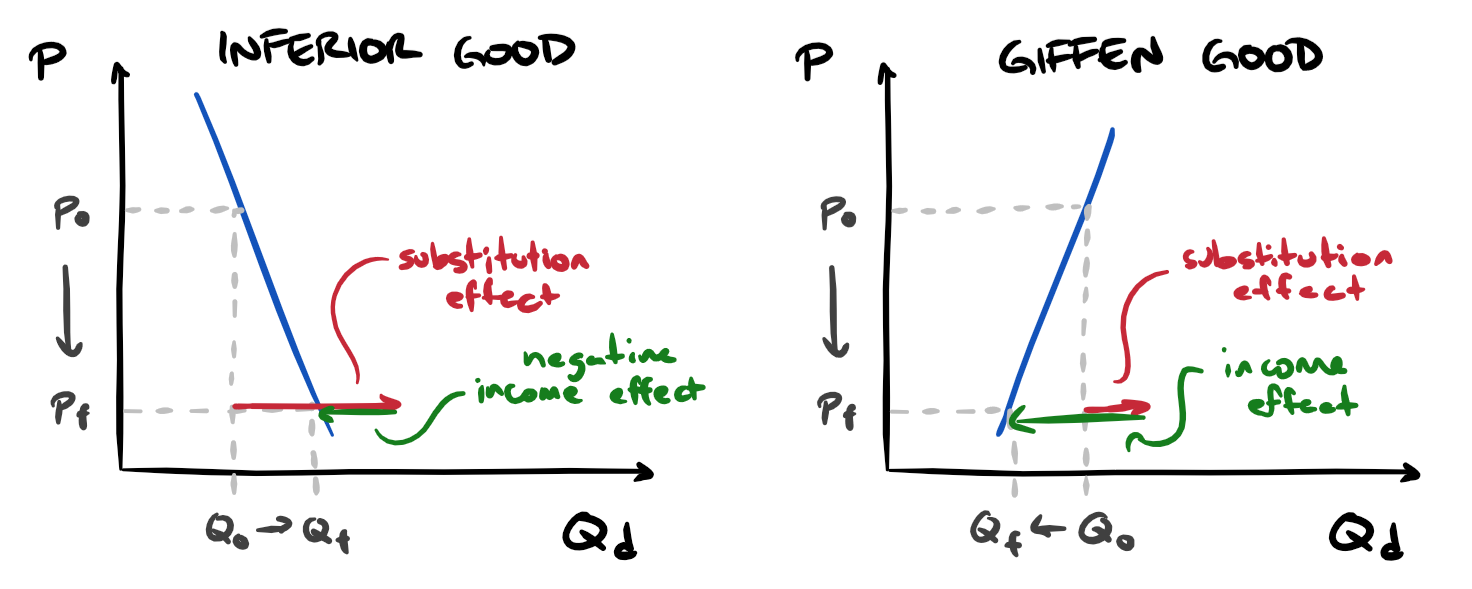
\includegraphics[width=140mm]{sub-inc-inf-gif.png}
\caption{Substitution Good of Inferior of Giffen Goods}
\end{figure}


Let's also address conspicuous consumption goods. These are goods that have "snob appeal". It is these goods, like diamonds, that are consumed simply because they are expensive, and if they became cheap people would be less interested. These seem to contradict the demand curve too. However, they don't violate it because these people find utility in the snob appeal. What they're really paying for and getting happiness from, is what people think. If the good became cheaper, people be as impressed, so in terms of utility from status, it would be worth less.

\subsection{Consumer Surplus}

When it costs less to buy than you would be willing to pay, the difference is called consumer surplus. If you were willing to pay \$3 for coffee, but they actually cost \$2, you would have \$1 of consumer surplus. 

As we know from the law of diminishing marginal utility, for each successive coffee consumed, the value placed in that coffee is less. So for a second coffee you might only be willing to pay \$2.50, and so you'd get a surplus of \$0.50. Eventually the value placed on the coffee will be less than the market price.

\begin{figure}[ht!]
\centering
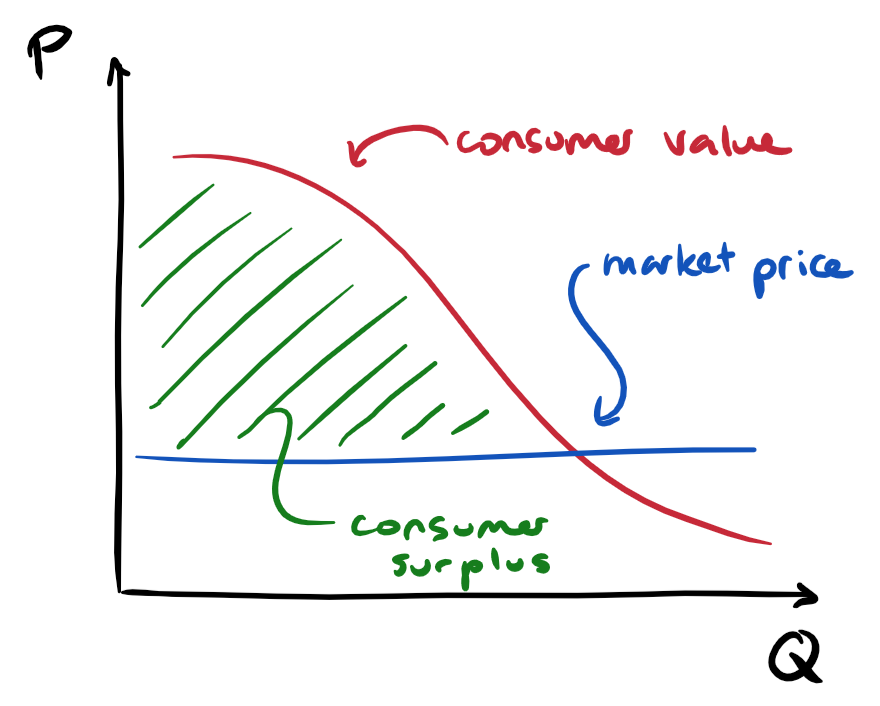
\includegraphics[width=80mm]{consumer-surplus.png}
\caption{Consumer Surplus}
\end{figure}

When you plot it out on a $P$ vs. $Q_{consumed}$ curve, the total area under the demand curve and above the market line is total consumer surplus.

\subsubsection{The Paradox of Value}

Everyone needs water to survive, but no one really needs diamonds. So why are diamonds so much more expensive than water? Great question. It has to do with the difference between total value and marginal value. 

Goods that are plentiful, like water, will be consumed until the point when the consumer surplus is nothing -- ie. when they value it at market price. This means they people are consuming the product even when they have a low value for it. 

Goods that are scarce, like diamonds, will stop being consumed early. This means that people stop consuming it when they still have a high value for it.

This same paradox exists in other markets, including labour. For example professional soccer players earn lots more than doctors, even though when push comes to shove you'd value having a good doctor more than watching a good soccer player.

Basically it just has to do with supply.



\subsection{Indifference Theory}

\subsubsection{Indifference Curve}

The indifference curve shows the combinations of two goods that would give a consumer the same amount of happiness. For instance, I'd be equally happy with three beers and two slices of pizza as I would be with one beer and five slices of pizza. It's along this curve that what you gave up has the same utility as what you got -- the two beers lost has the same utility as the three gained slices of pizza. 

\begin{figure}[ht!]
\centering
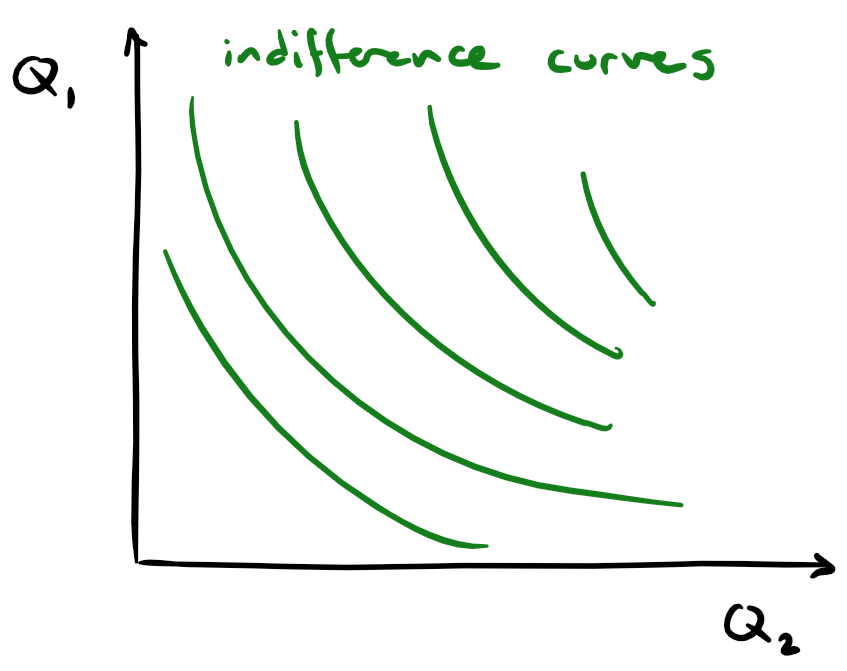
\includegraphics[width=80mm]{indif-map.png}
\caption{Indifference Curves (Map)}
\end{figure}

The reason the curve is convex to the origin is because of the diminishing marginal rate of substitution. The amount beer you'd be willing to give up for more pizza decreases as you get more pizza, and vice-versa. 

Above the curve means you're getting extra satisfaction, below the curve you're getting less satisfaction. The indifference curve can be drawn at different level of utility, creating an Indifference Map. When an economist says that a consumer's tastes are given, they mean they have their indifference map.

\subsection{The Budget Line}

Like the indifference curve, the budget line shows the combination of two goods. But instead of the combinations of the good the consumer values equally, it shows the combinations of the good the consumer can afford. For that reason, it's a linear negative curve.

The relative price, $$P_x/P_y$$ determines the slope. It reflects the opportunity cost in terms of the two goods.

\subsection{Consumer Utility Maximizing}

Combining the indifference curve and the budget line, we see what combinations the user wants and what they can afford. The best combination for the user is the point where the budget line is tangent to the indifference curve. When they're tangent, it means that they're as far outward (getting the highest utility) as possible, and they have the combination that they can afford and want.

\begin{figure}[ht!]
\centering
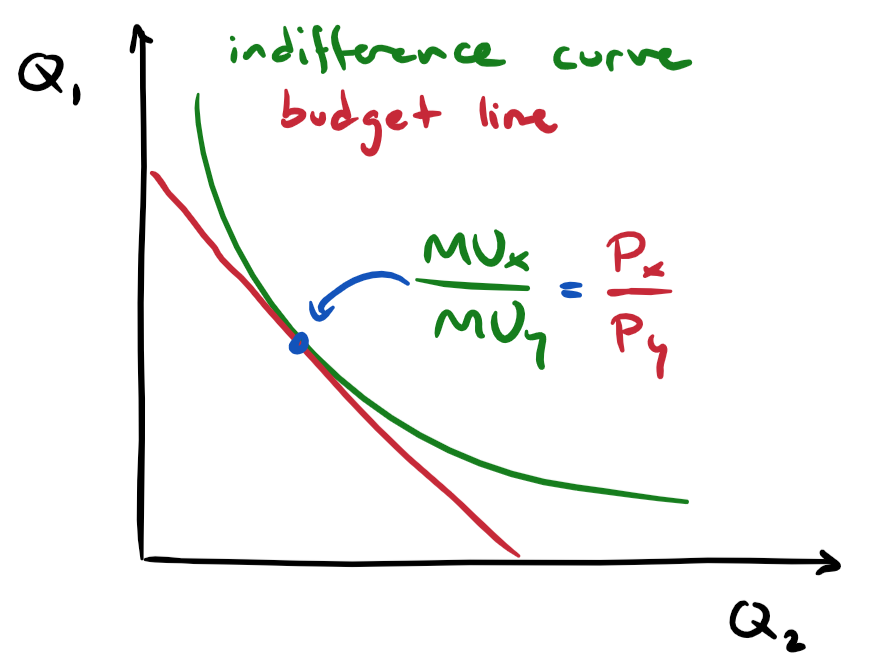
\includegraphics[width=80mm]{indif-bl.png}
\caption{Indifference Curves and Budget Line}
\end{figure}

\subsubsection{Income-Consumption Line}

If the consumer gets more real income, it shifts the budget line outward because now they can afford greater quantities of things. As this happens, the tangent point of each indifference curve can be traced out. This tracing is the income-consumption line. It neatly shows how the consumer's purchases would change in response to change in real income.

\subsubsection{Price-Consumption Line}

If there's a change in the relative price of the goods, that causes a rotation (not a shift) of the budget line. Same as with the income-substitution line, if you trace out the points at which the budget line is tangent with the indifference map curves it creates a  line. This line is the price-consumption line, and it shows how the consumer's purchases change in response to changing relative prices.


\begin{figure}[ht!]
\centering
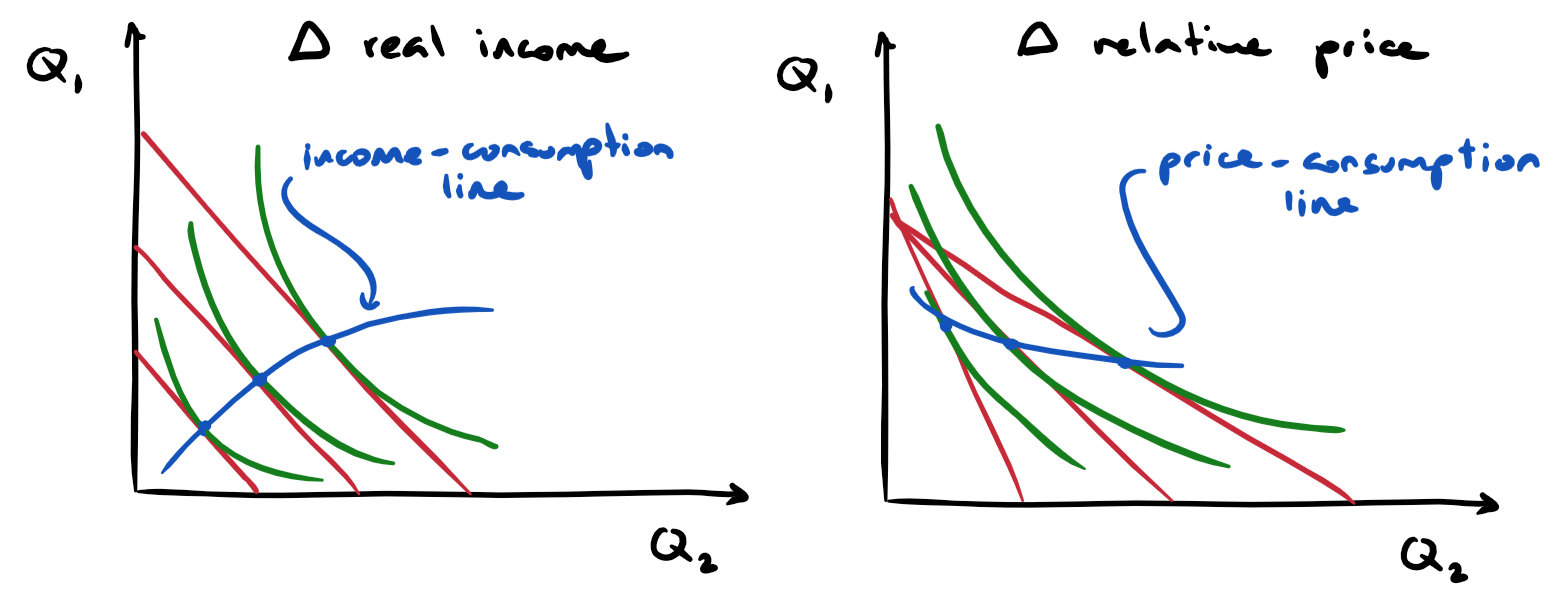
\includegraphics[width=120mm]{income-price-consumption-lines.png}
\caption{Income and Price Consumption Lines}
\end{figure}

Note that every point en the price-consumption line, corresponds to a quantity demanded and a price of a product. If you graph these, you'll create the demand curve.

\subsubsection{Income and Substitution Effect}

The income and substitution effect can be seen in changes of the budget line and price consumption line. After the price of a good has fallen, assume you reduce income so that the budget line can just reach the original indifference curve. At that point, the change in quantity is due to the substitution effect. Then, you can restore the income to reach the new indifference curve. The additional quantity is due to the income effect.


\begin{figure}[ht!]
\centering
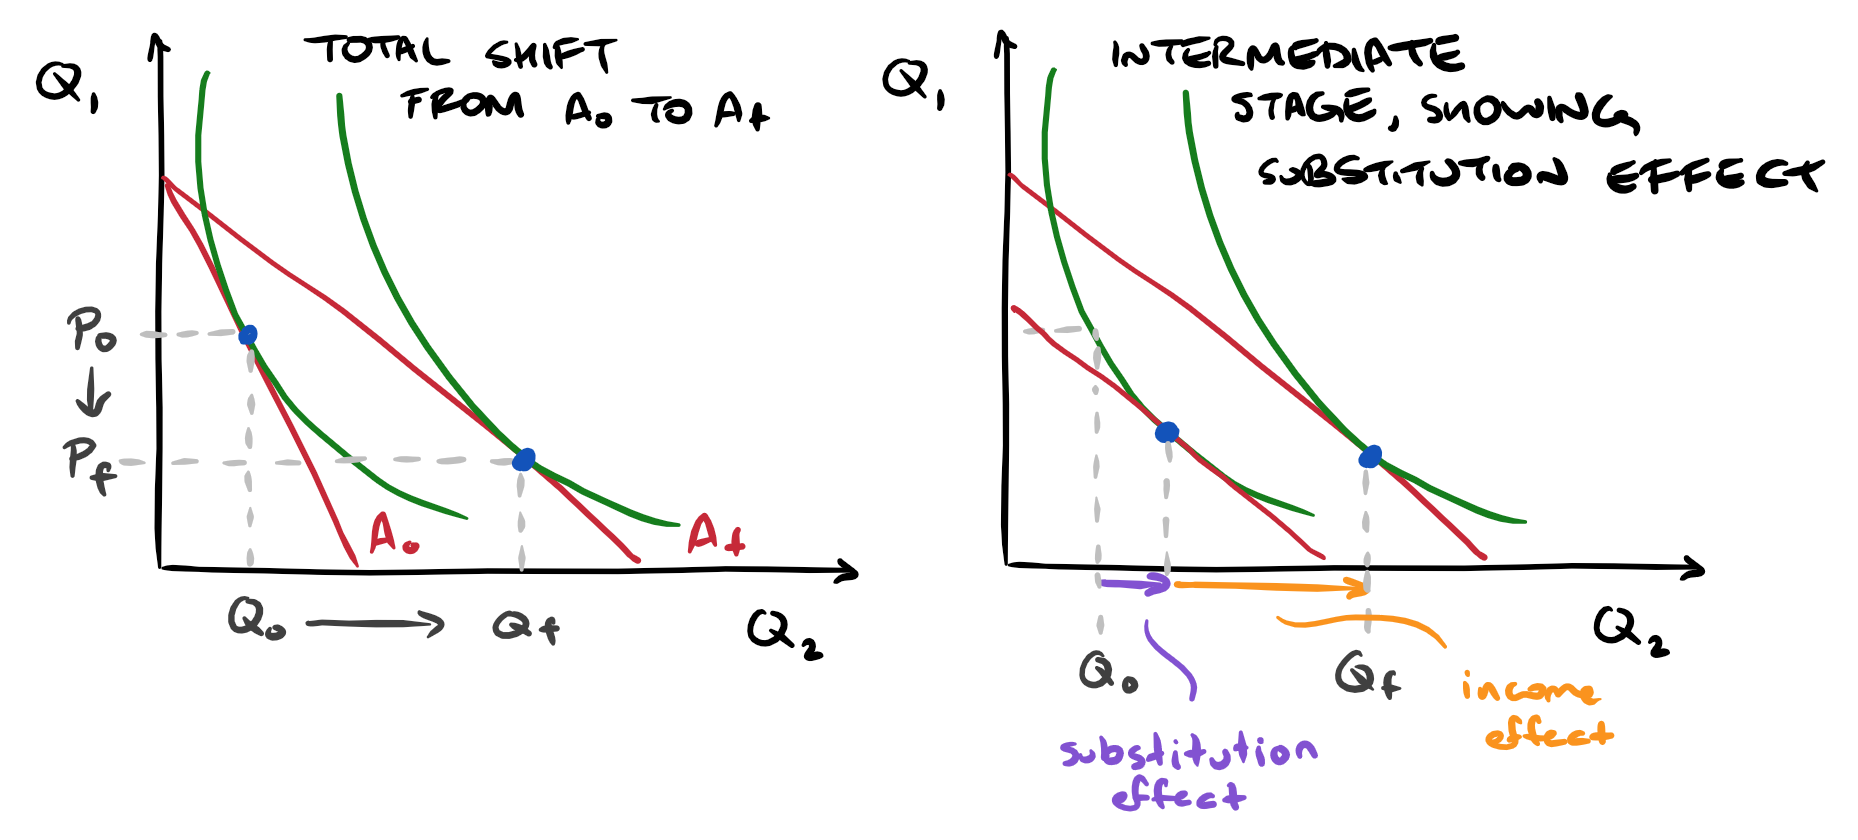
\includegraphics[width=120mm]{substitution-effect-with-bl-indif-curve.png}
\caption{Substitution Effect on Budget Line/Indifference Curve}
\end{figure}

\section{Firms}

We assume that firms 1) try to make as much profit as possible, and 2) is a single, consistent decision-making unit. With these assumptions we can predict their behaviour. The main types are Sole Proprietorship -- where the business and the individual are one, and the owner is personally liable for the business; Partnership -- a group of sole proprietors;  and a Corporation -- where the firm has its own legal entity and the owners have limited liability for it.

\subsection{Financing of Firms}

Firms can be financed with Equity Financing or Debt Financing. 

Equity Financing is when people gift the company money in exchange for some share/stock of control of the company. There's no guarantee they'll get the money back, but sometimes are given a share of the profits in the form of dividends. 

Debt Financing is when the company's creditor's aren't the owners. Rather, the company is loaned money, called bonds, and the company promises to pay back the creditor with interest. 

\subsection{Production, Cost, and Profits}

The production function maps the inputs, capital $K$ and labour $L$, the the output $Q$. Explicit costs are things that actually involve purchasing goods or services. Implicit costs are the opportunity costs of business, like taking a lower paycheck when starting a company instead of working for another firm, or running the business instead of liquidating the capital to simply invest it. 

$$Profits_{accounting} = Revenues - Costs_{explicit}$$

$$Profits_{economic} = Revenues - Costs_{explicit} - Costs_{implicit}$$

Firms are interested in how much return they're making for their owners. But economics are interested in efficiently allocating resources based on opportunity-cost. When their are economic profits, that signals that resources should be moved into that industry.

\subsection{Time Horizons}

Decisions that firms have to make are categorized into three categories, short run, long run, and very long run. These don't really have much to do with actual time periods, but rather what can be held constant during those horizons. 

Short run assumes that some factor of production, often capital, is fixed, and some other quantity, often labour, is variable.  Long run assumes that all inputs except technology are fixed. Many planning decisions are based on long-run, assuming the technological possibilities will not change. The very long run assumes that all factors of production, including technology can change. 

\section{Production in the Short Run}

\subsection{Total, Average, and Marginal Products}

Total product $TP$ is the total amount that is produced in a given period of time. The average product $AP$ is the total product divided by the number of units of the variable factor, for instance labour. The average product will reach a maximum at the point of diminishing average productivity. Beyond that point, the average product is decreasing. 

Let's say you have five workers who between them can make twenty shirts a day, then they have an average product of 20/5 = 4. However, let's say you add some more workers, and suddenly they start bumping into each other, so you have ten workers producing 35 shirts a day. Then you have an average product of 35/10 = 3.5, so even though you're making more, your average product is decreasing. 


\begin{figure}[ht!]
\centering
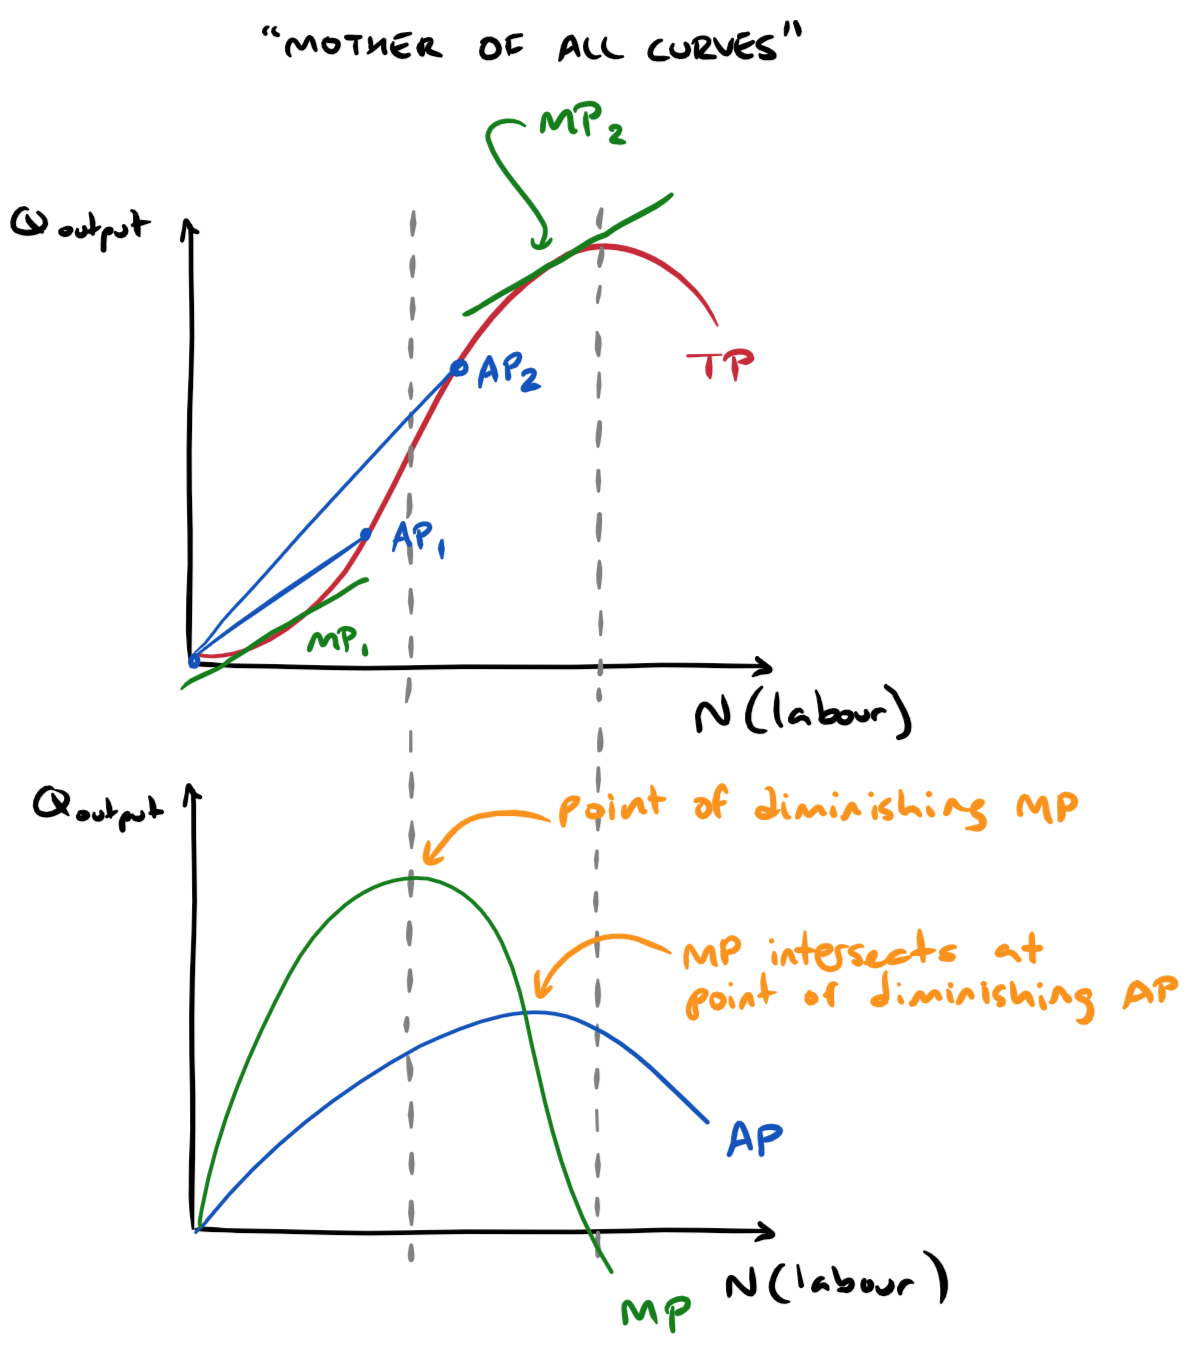
\includegraphics[width=90mm]{MOAC.png}
\caption{Total, Average, Marginal Utility Curves (MOAC)}
\end{figure}


Marginal product $MP$ is the change in total product resulting from one additional unit in labour, $MP = \Delta TP / \Delta L$. This is basically the derivative of the total product curve, it shows how steeply the $TP$ rises based on your variable factor, here we again used labour. Notice that the marginal product intersects the average product at the average product's peak. This is because when the marginal product is above the average product, each additional unit of labour will increase average product. But when the marginal product is below the average product curve, the additional units will create a decreasing average product.

\subsubsection{Diminishing Marginal Product}

The law (actually hypothesis) of diminishing marginal returns says that as you increase your variable factor, eventually the marginal product will reach a max and start declining. This isn't when the average product begins to decline, it's when the increase of $TP$ with the fixed factor stops accelerating. Let's say your workers are creating T-shirts, as you add more workers they can specialize with division of labour and become more efficient so marginal product will rise. Eventually though, the additional worker doesn't make everyone as a whole more efficient. 

\subsection{Costs in the Short Run}

Total cost $TC$ is the sum of all costs. Total fixed cost $TFC$ is the overhead cost to run the operation, and it's constant. Total variable cost $TVC$ is based on the level of output, it's basically the cost per unit produced. 

Average fixed cost $AFC$ is the total cost divided by the quantity of output $AFC=TFC/Q$, it actually continuously declines as production increases. Think of it like this -- if you have to pay a fixed rate of 50 dollars per month to run your banana stand, if you sell 10 bananas, your average fixed cost is 5. But if you sell 50 bananas, your average fixed cost is 1. Basically, as you increase production, those fixed costs are doing more for you, so they decrease.

Average variable cost $AVC$ is the total variable cost divided by the output $AVC=TVC/Q$. This declines as output rises then reaches a minimum and starts rising again. Average total cost $ATC$ is the sum of $AVC$ and $AFC$.

Finally, marginal cost $MC$ is the increase in total cost from an increase in one quantity out output $MC=\Delta TC / \Delta Q$.

\subsubsection{Short Run Cost Curves}

\begin{figure}
\center
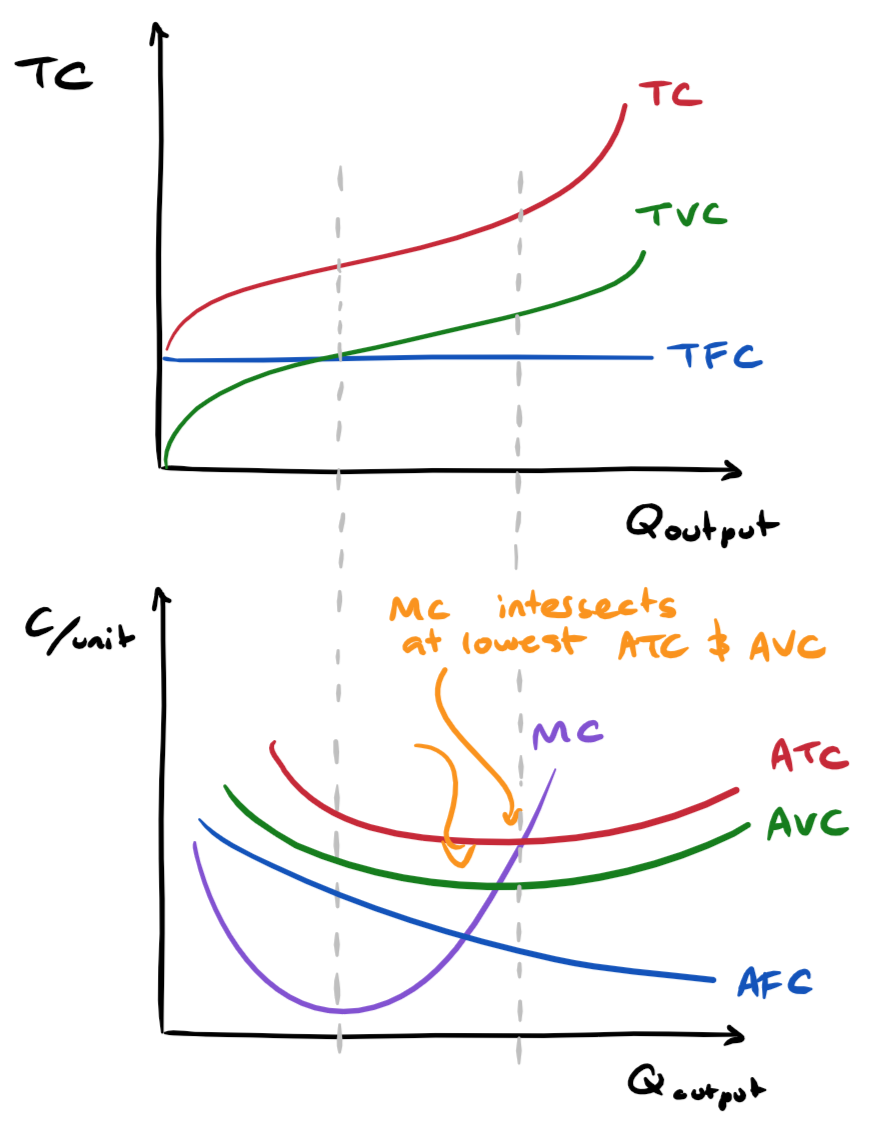
\includegraphics[width=80mm]{cost-lines.png}
\caption{Total, Average, Marginal Cost Curves}
\end{figure}

Note that $MP$ and $AP$ are both hill shaped, whereas $AVC$ and $MC$ are both U-shaped. At the quantity associated with the minimum value of of the $ATC$ is called the capacity of the firm. It's the largest level of output that can be produced without increasing average cost. Firms are said to be above capacity when they will pay the additional average costs per unit in order to produce even higher quantity.

An increase in the price of the variable factor, for instance a minimum wage, would shift the short run costs curves upward. Changes in the fixed factor create completely new curves, for instance an increase in plant size could shift cost up but also increase capacity.

\section{Production in the Long Run}

When we say the long run, we mean the period in which we consider all factors except technology free to vary. This results in the combination of many different short run cost curves. The long run sets out to determine which short run cost curve to use. 

There are numerous ways to produce a given output, you can use one engineer and lots of automated robots, or lots of labourers and no robots, or somewhere in between. Technical efficiency means minimizing the number of inputs to produce a given output. 

\subsection{Profit Maximization and Cost Minimization}

We're going to assume that the firm has a specific output it needs to meet, so the best way to maximize profits is to minimize costs of production. To do this, the marginal product per dollar of factor of production should not exceed the marginal product per dollar of another factor of production. In other words, if you're getting more bang for your buck by investing in capital over labour, invest more in capital. If you're getting more bang for your buck by investing in labour over capital, invest more in labour.

$$\frac{MP_K}{P_K} = \frac{MP_L}{P_L}$$

Whenever these ratios are imbalanced, there are opportunities to substitute factors and reduce costs. The prices of the factors are given by the market, so you can't control those. The only way to control this equation is by investing in the factors to change the marginal products.

Remember, the law of diminishing marginal returns says that (assuming other inputs held constant) the more you invest in one factor, the smaller that factor's marginal product will be. 

So let's say $\frac{MP_K}{P_K} > \frac{MP_L}{P_L}$, that means for every dollar you spend on capital, you're getting more marginal product. So you should invest more in capital. As you invest more in capital, the marginal product of capital $MP_K$ decreases so the equation will again equalize. 

\subsection{Long-Run Cost Curves}

With given factor prices (not quantities), there is a minimum achievable cost for each level of quantity output. The long-run average curve $LRAC$ shows these costs. Its axes are cost per unit of product, and the quantity produced. Its shape and position are determined by the current level of technology and the prices of the factors of production. 

To move from one point to another, it requires changing the quantities of all factors of production. 

\subsubsection{(Dis)economies of Scale}

\begin{figure}
\center
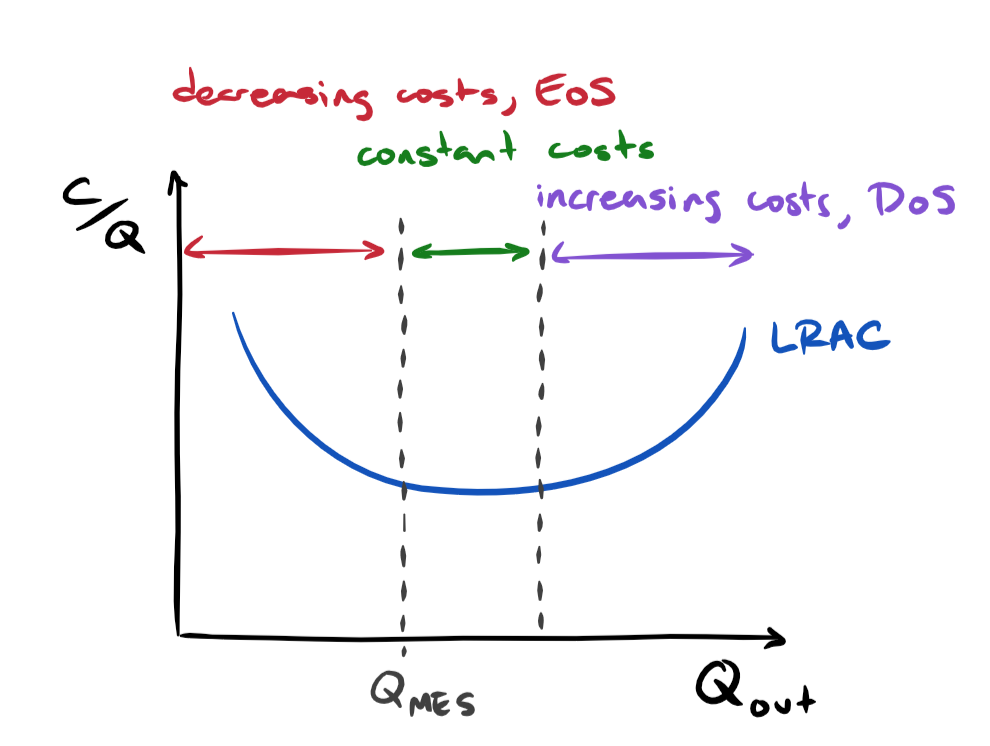
\includegraphics[width=80mm]{1030 diseconomies of scale.PNG}
\caption{Long Run Average Cost Curve}
\end{figure}

In the leftmost section of the curve, the cost per unit is decreasing with the level of output. This means the more you're producing, the cheaper it is to produce each product and is called economies of scale, or increasing returns.

Some reasons you might get economies of scale is that your fixed costs/overhead costs are going further, so your average fixed costs is diminishing. Or think of a plane, the pilots salary is the same whether he's flying a jumbo jet or a little prop-plane, but your quantity is much larger so your costs are less. It's tempting to say division of labour here, but Gateman seemed to not really like that answer and considered it more suitable to the SRAC curve.

Then in the middle of the curve you have what are called constant costs/constant returns. They're pretty boring. 

Then on the rightmost of the graph, the quantity of output is increasing less than in proportion to the increase in inputs. These are called diseconomies of scale, and it means the more of something you produce, the more expensive it gets per unit. This can happen if companies grow out of control. A reason for diseconommies of scale is that as companies grow larger, they tend to hire more middle management and extra people who aren't really producing, like HR people or workplace counsellors. In small businesses, everyone plays a big role and is really invested in the company, as it grows larger people tend to be alienated and inefficient because they're just one of hundreds. 

\subsubsection{Relationship Between SRAC and LRAC}

The LRAC curve is formed from the envelope of all the SRAC curves. No SRAC curve can fall belew the LRAC curve, at each point along the LRAC  curve there are tangent SRAC curves. 


\begin{figure}
\center
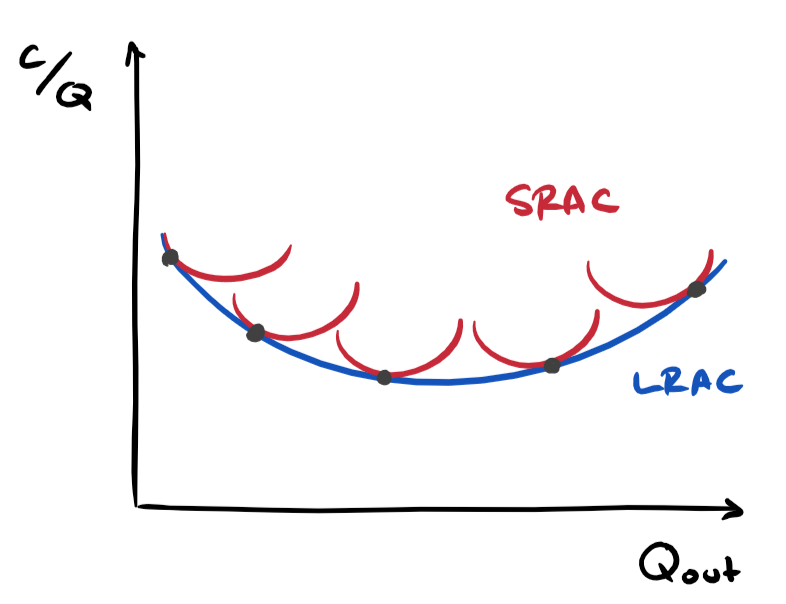
\includegraphics[width=80mm]{1033 SRAC LRAC.PNG}
\caption{Long Run Average Cost Curve Envelope}
\end{figure}

\subsubsection{Shifts in the LRAC curve}

Rises in factor prices shift the LRAC curve upward. Technological improvements can shift the LRAC curve downward. 

\subsection{The Very Long Run}

The very  long run as when all factors are variable, including technology. Productivity is measured as the output produced per unit of input (often output/worker or output/hour are used).

Changes in technology are put into practice by firms in search of profits. The three kinds of changes in production and cost in the very  long run are new techniques; improved inputs; and new products. 

When faced with price increases of a factor, firms either substitute away or innovate away from the input. For instance, let's say labour costs rise -- A company can either substitute away and start hiring labourers in cheaper countries; they can substitute away and start buying capital to replace labourers; or they can innovate away by devoting resources to developing new automation technologies. 

\subsection{Isoquant and Isocost Analysis}

This is sort of like the budget line and indifference curve analysis featured previously, except now from the perspective of producers instead of consumers. 

In isoquant line is analagous to the indifference curve. It is the curve at which any two possible combinations of inputs (again, let's use labour and capital) can produce a set level of output. Like the indifference curve, it's a downward sloping convex curve. Downward sloping because whenever you move away from one factor, in order to keep up production at the set quantity you need to invest more in the other factor. It's convex because our friend the law of diminishing returns tells us that the more you invest in labour for instance, the less marginal return labour gives you, so you have to add more to keep the same level of productivity.

\begin{figure}
\center
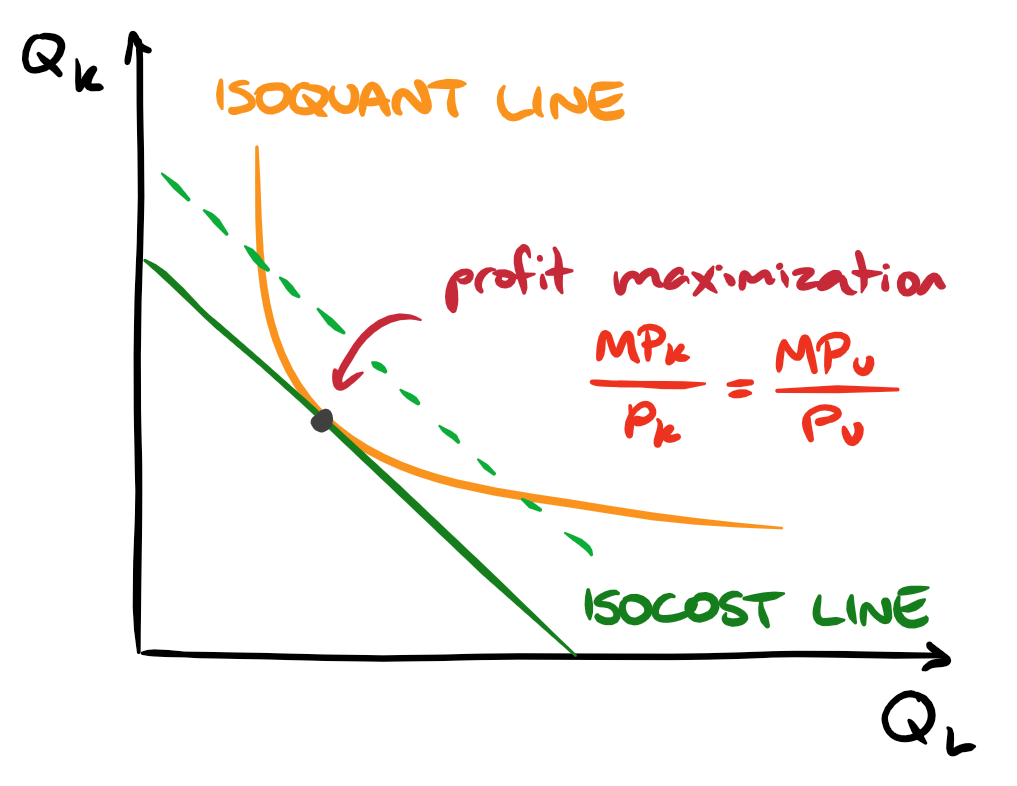
\includegraphics[width=80mm]{1064 Isoquants.PNG}
\caption{Isoquant and Isocost Lines}
\end{figure}

The isocost line is analgous to the budget line,  it is the alternative combinations of the factors that a company can afford. So given the combinations of the factors that produce a certain level of output, and the cost of the combination of factors that can be afforded, the way to minimize cost is to find the isoquant line tangent to the isocost line. This should look familiar by now:

$$\frac{MP_L}{MP_K} = \frac{P_L}{P_K}$$

An increase in the price of one factor changes the slope of the isocost line, and the new isoquant line must be found that is tangent to it. 
 
There is one major difference between the isoquants and the indifference curves though. When discussing indifference curves, usually our budget line (the linear line) is fixed and we must find the appropriate indifference curve at which we're happiest.

When discussing isoquants, usually the isoquant line (the curved line) is fixed and we must find the appropriate isocost line at which we're happiest. 


\section{Perfectly Competitive Markets}

It's interesting to note that despite the name, there  is no competition in perfect competition. This is because there is no competitive behaviour among firms, because no firms have \textit{market power}, that is, no firms can effect the price of their product. 

In this case, the price of the product is set by the equilibrium price of the market demand and supply curves. The only way for producers to influence their profits is to reduce costs. Perfectly competitive markets are the only market structure that do not have a negatively sloped demand curve, rather it is horizontal. 

\subsection{Assumptions of Perfect Competition}

A perfectly competitive market requires fours characteristics.

\begin{enumerate}

\item All firms sell a \textit{homogeneous product} (the same thing)

\item Consumers know the prices charged by each firm

\item Each firm is small relative to the industry (can't change market S curve)

\item There are no barriers to entry or exit for firms
\end{enumerate}

Assumptions 1-3 ensure that the firm is a \textit{price taker}, ie. can change how much it sells without changing the market price. In other words, even though the industry as a whole as a negatively sloped demand curve, the individual firm demand curve is horizontal (perfectly elastic). This is because the change in output of a single firm has no perceivable effect on the output of the total industry. 

For a price taking firm therefore, price, marginal revenue, and average revenue are all the same horizontal line, $P = MR = AR$.

Assumption 4 ensures that the firm produces at the minimum cost on the LRAC curve.

\subsection{Short--Run Decisions}

In the short run, there is a fixed number of firms and each firm has a fixed plant size. The firm first has to decide whether 1) it should produce at all and 2) how much to produce. 


The firm should continue to produce if $TR > TVC$ or $P > AVC$, then they have enough to cover day-to-day expenses and then some. \textit{Shut-down price} is the price at which the firm is is just covering the costs of production $P = AVC$. 

The firm should produce a quantity such that $MR = MC$. If the marginal revenue exceeds the marginal cost, then the firm can get more profits by increasing production to the point where they are equal. If the marginal cost exceeds the marginal revenue, then additional production is not worth it and they should dial it back. Recall that for a price-taking firm, $MR = P$. 

\begin{figure}
\center
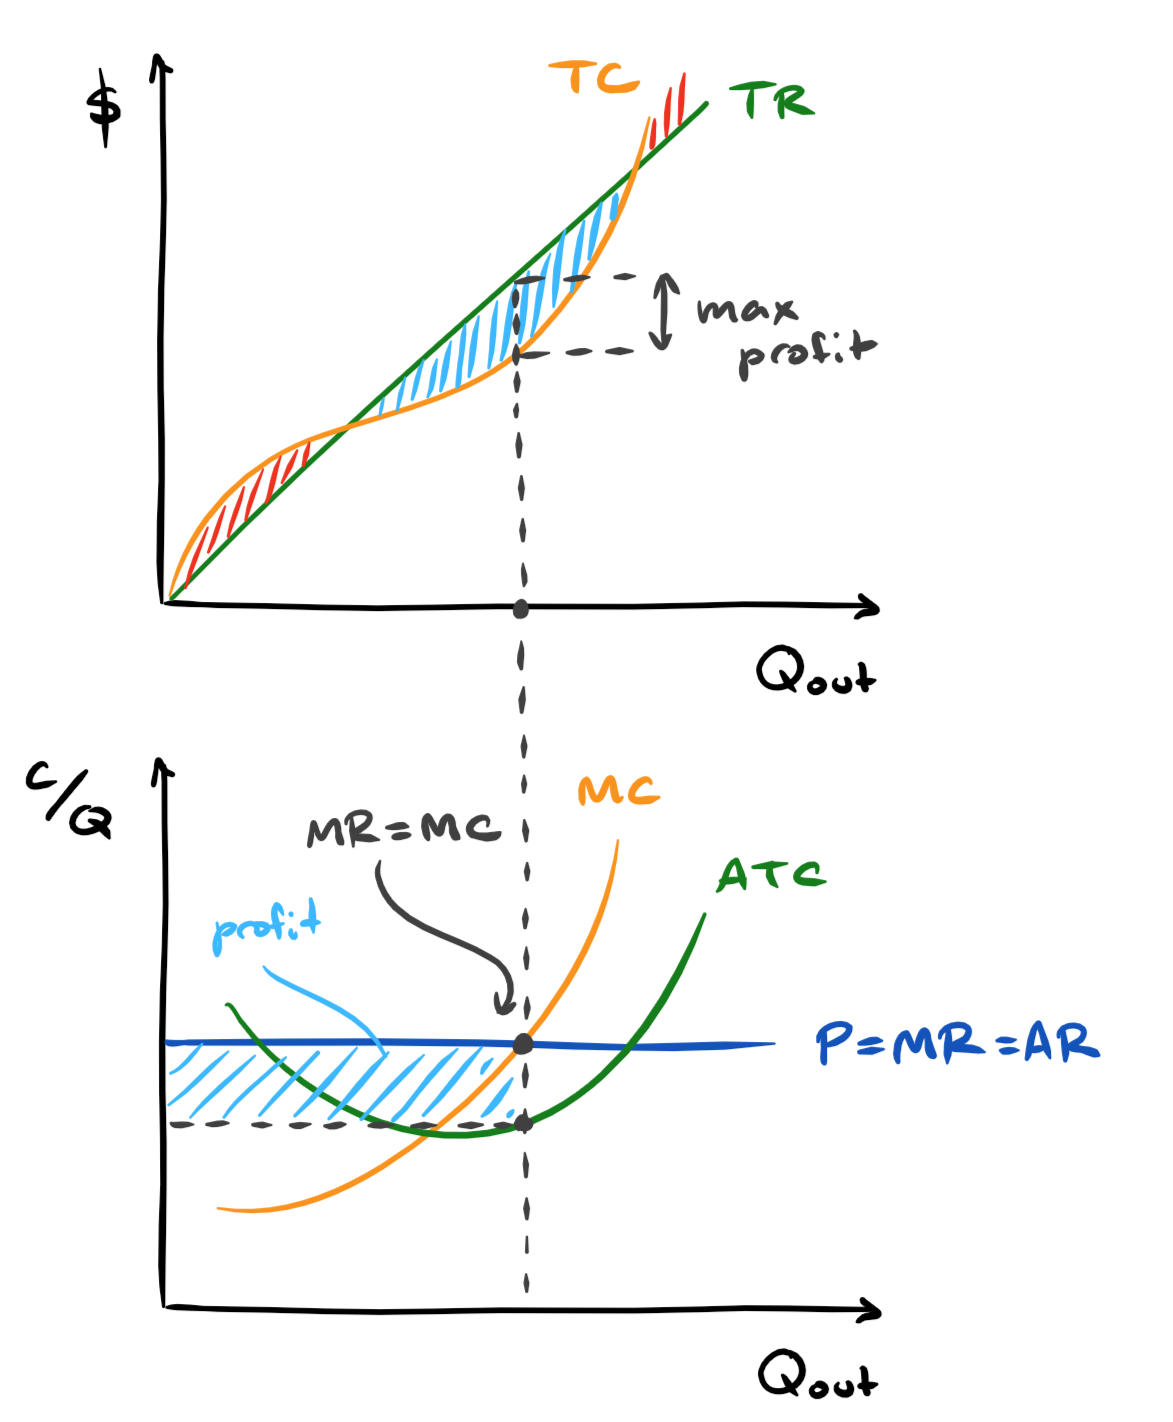
\includegraphics[width=80mm]{1119 profits.PNG}
\caption{Profit Maximization of Competitive Market}
\end{figure}

As you can see, the point at which $MC = MR$ is the point where profits are maximized, as long as $P > AVC$. So a firm in a perfectly competitive market chooses the level of output at which profits are maximized. 

The supply curve of a firm is the MC curve above the AVC.  

\begin{figure}
\center
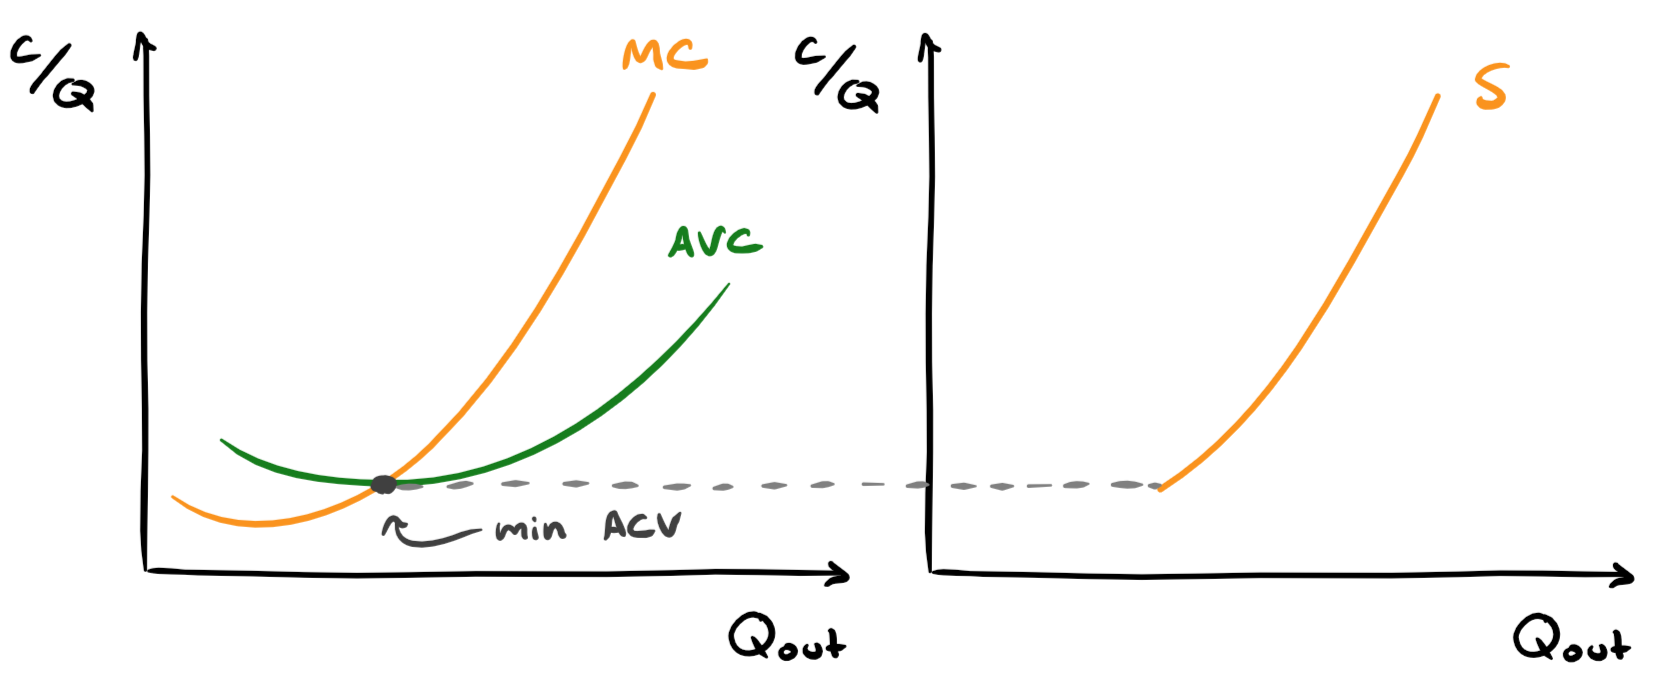
\includegraphics[width=110mm]{1119 supply AVC.PNG}
\caption{Origin of Supply Curve}
\end{figure}


\subsubsection{Short--Run Equilibrium}

The price of the product in a perfectly competitive market is determined by the intersection of the supply and demand curve, ie. $Q_d = Q_s$. In the short run, a profit maximizing firm will be producing the $Q$ at which $MC = MR$ and will have no motivation to change. 


\begin{figure}
\center
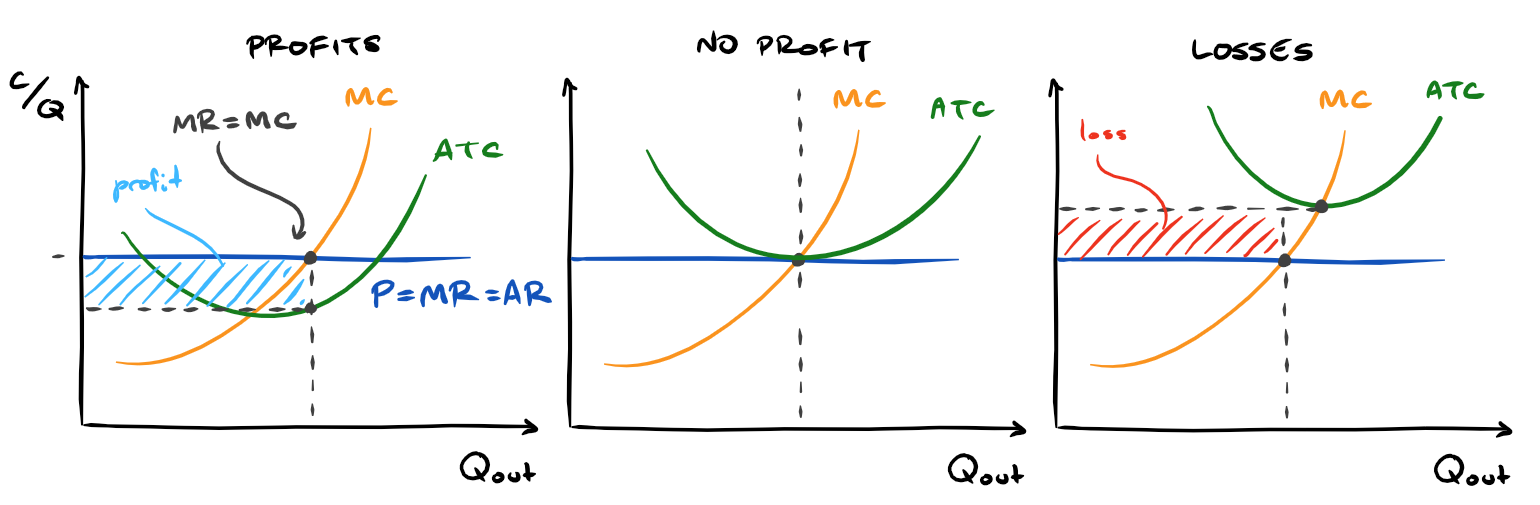
\includegraphics[width=130mm]{1125 short run profits normal loss.PNG}
\caption{Positive Profits, Normal Profits, Losses of in Competitive Market}
\end{figure}


In all cases above, the firm is maximizing its profits by producing where marginal cost equals marginal revenue/price. Profit is the difference between price and average total cost, $Profit = TR - TR = Q(P-ATC)$. 

Some firms will continue producing despite making losses, because the firm will still have to pay fixed costs and can minimize losses by producing as long as $P > AVC$. For instance, in the off-season a hotel may be operating at a loss, but it would have to continue to pay fixed costs such as property taxes if it closed down. So it may be more profitable to continue to operate at a loss in order to decrease total losses. 

\subsection{Long--Run Decisions}

In the long run, both the number of firms and the size of each firm's plant size is variable, however technology is fixed. In the long-run, we must account for the entry and exit of firms. 

\subsubsection{Entry and Exit of Firms}

If the firms in an industry are making economic profits, that will motivate new firms to enter the industry. This will shift the industry supply curve right, decreasing the equilibrium price. This will continue until all the firms are only making \textit{normal profits}, ie. just making enough to cover their total costs. 

\begin{figure}
\center
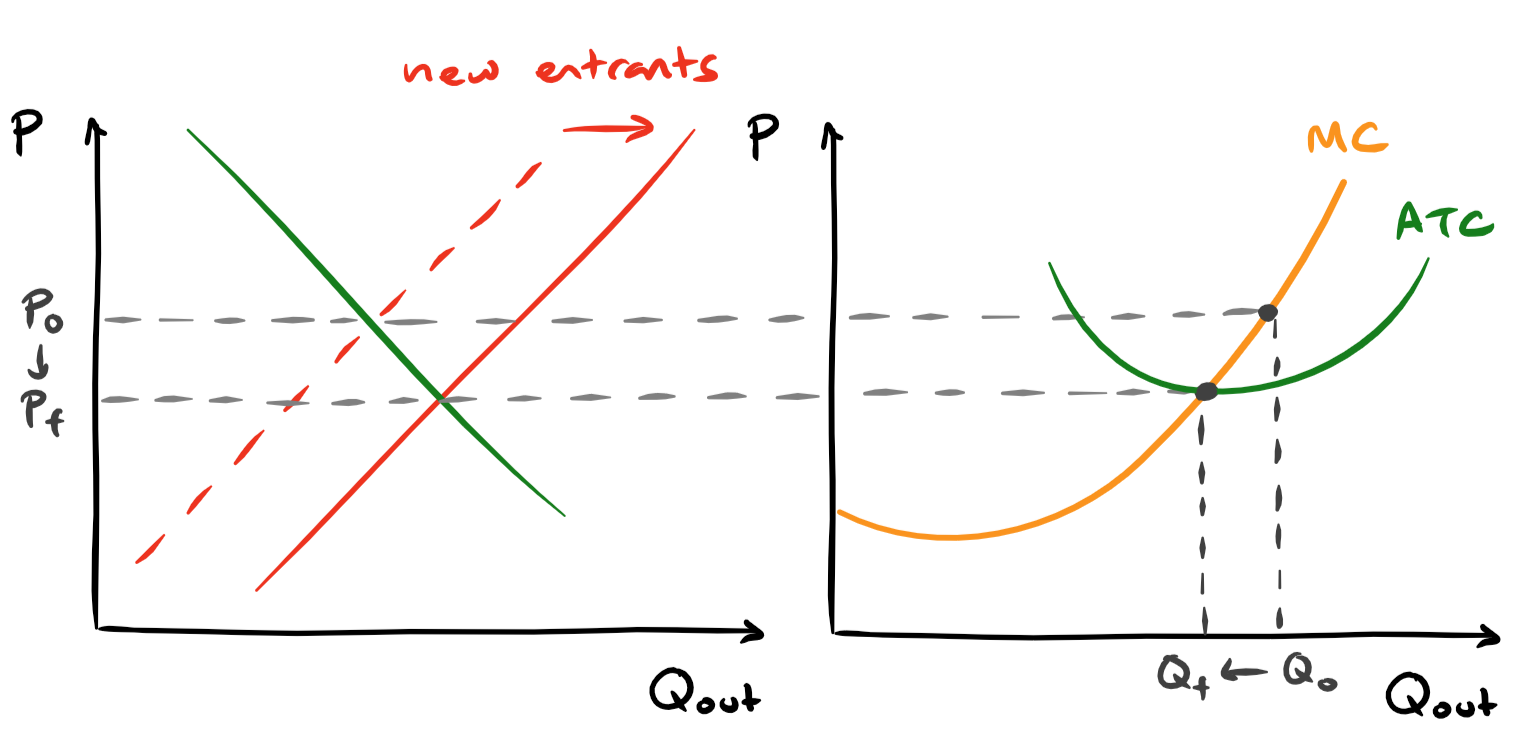
\includegraphics[width=100mm]{1139 entry of firms.PNG}
\caption{Entry of Firms in Long Run}
\end{figure}


On the otherhand, if the firms are making economic losses, that will motivate existing firms to leave the industry, driving the market supply curve left and raising the price. This will also continue until the firms are only making normal profits. 


\begin{figure}
\center
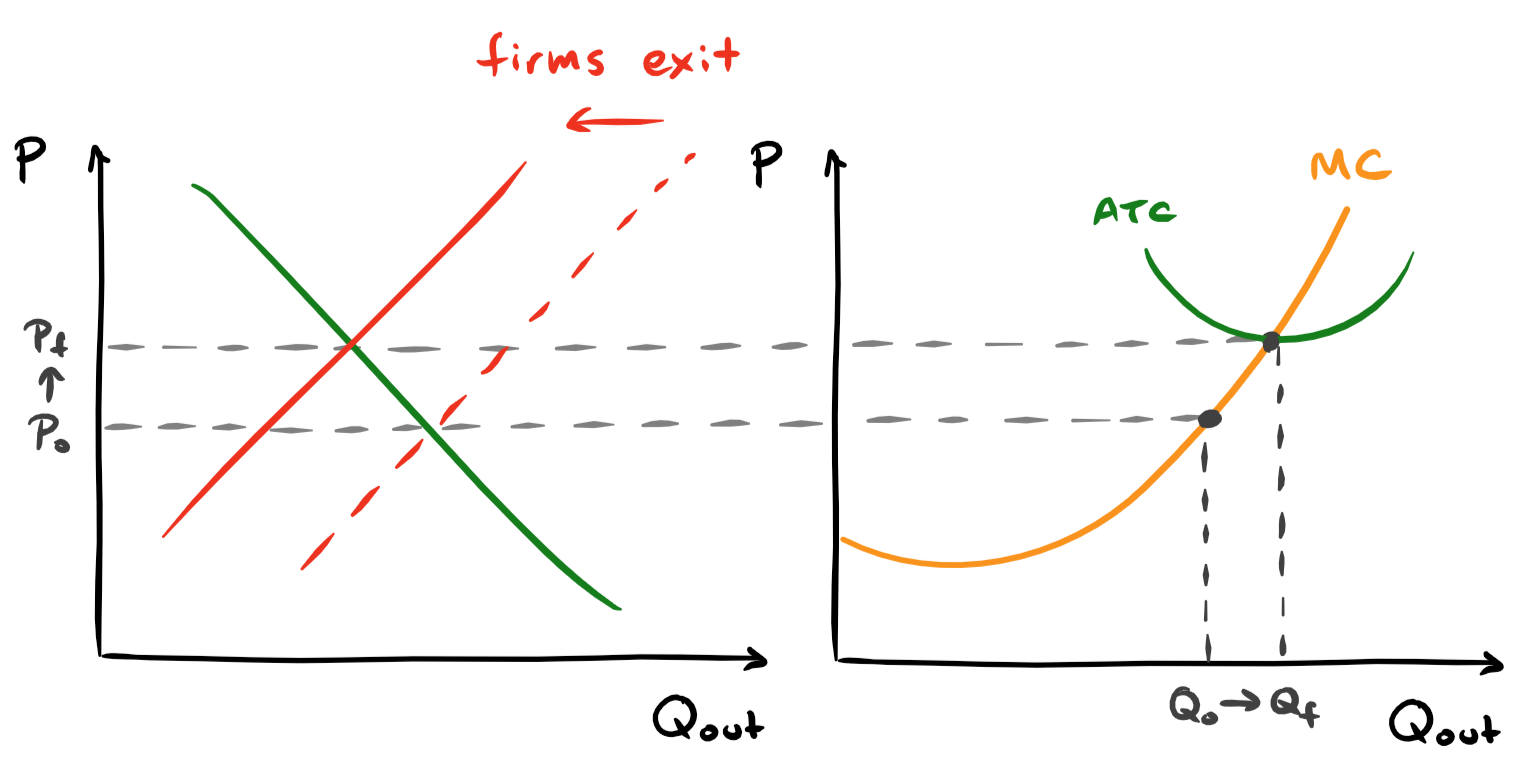
\includegraphics[width=100mm]{1144 exit of firms.PNG}
\caption{Exit of Firms in Long Run}
\end{figure}



\subsubsection{Speed of Exit}

The longer it takes for a firm's capital to become obsolete, the longer firms will remain in the industry even if they are making losses. For instance, railways take a longer longer to wear out or become obsolete than office equipment, so an office is more likely to shut down quickly after beginning to make economic losses. 

Similarly, if closing a firm can result in substantial salvage costs (non-sunk costs), that firm will exit the industry quicker than if the firm's costs are mostly sunk-costs. 

Because economic costs include opportunity cost of capital, if a firm is only just breaking even then they could increase their profits by shutting down and investing their capital elsewhere.


\subsubsection{Long--Run Equilibrium}

By the time the entry and exit of firms has ceased and all firms are earning normal profits, the industry is said to be in long-run equilibrium. Long-run equilibrium requires the following conditions.

\begin{enumerate}

\item Existing firms are maximizing their profits, $MC = MR = P$

\item Existing firms are not making losses or profits, so no firms are entering or exiting the industry, $P = SRAC minimum$. 

\item Existing firms are not able to increase their profits by changing the size of their plants, $P = LRAC minimum$. In other words, if the $LRAC$ curve was below the $SRAC$, the firm could lower its cost by increasing the scale of the plant. So the firm must be operating at the \textit{MES}. 

\end{enumerate}

\begin{figure}
\center
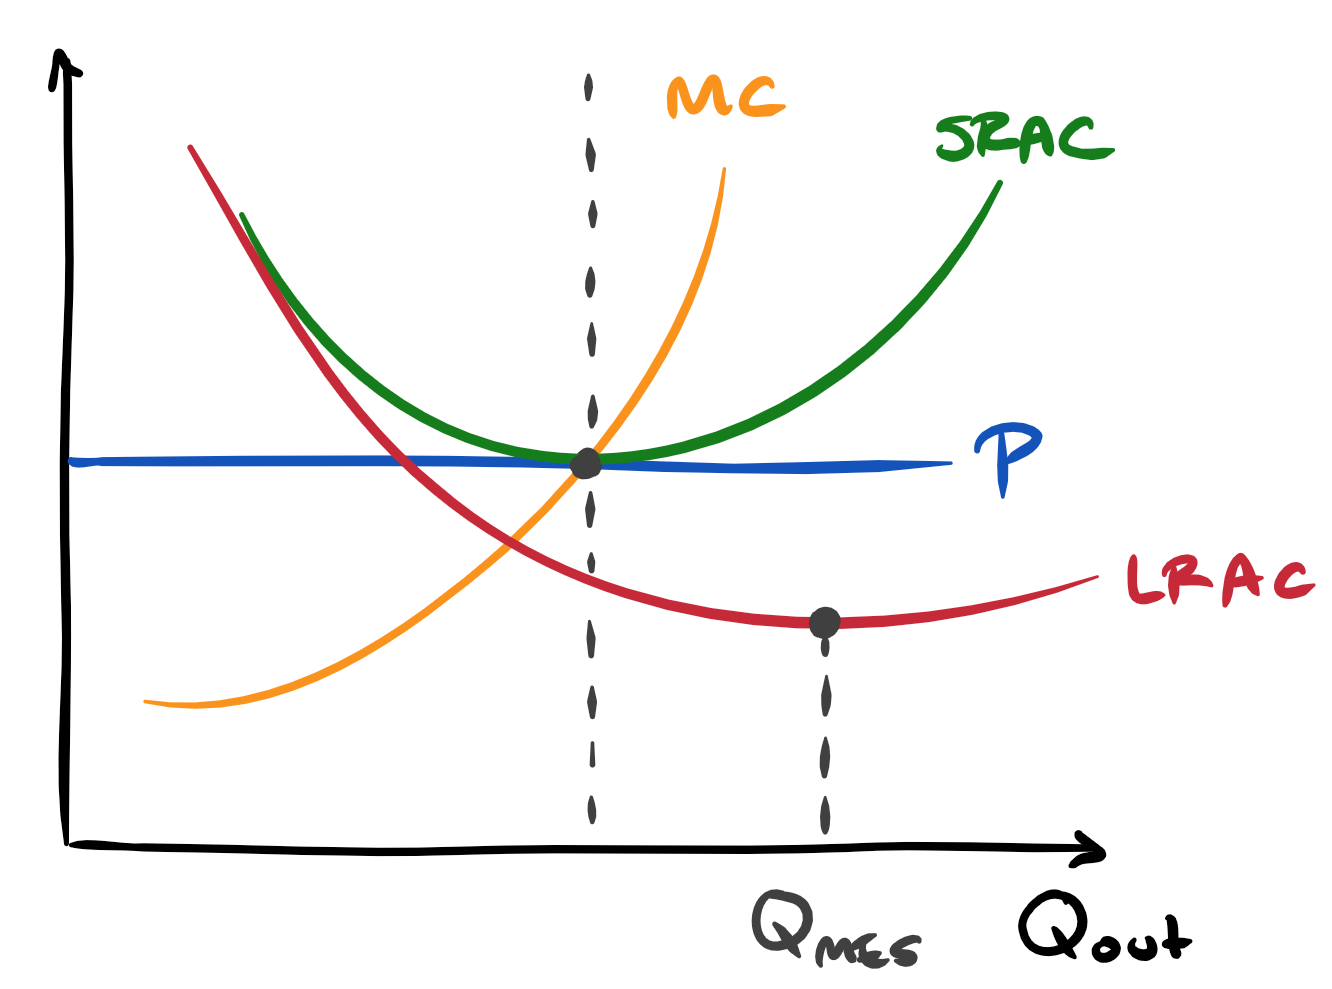
\includegraphics[width=80mm]{LRAC SRAC.PNG}
\caption{Short-Run vs. Long-Run Profit Maximization for Competitive Firm}
\end{figure}


All of this is to say that in long-run equilibrium, the firms costs are the lowest possible with the given technology. 

\subsubsection{Changes in Technology}

Improvements in technology would cause an increase in capacity, shifting the short run supply curve to the right and decreasing the price. The price will continue to fall until the firms with the new technology are only earning normal profit. At which point, the firms with the old technology will not be able to cover their costs and will leave the industry. Eventually a new long-run equilibrium will be established with all the plants using the new technology and selling at a lower price.

The older firms can still continue to operate as long as their revenues cover their variable costs, $P>AVC$. 



\section{Monopolies, Cartels, Price Discrimination}

A monopoly is when a single firm, called a monopolist, provides the output of an entire industry. A cartel is when multiple firms band together to co-operate as a monopolist in order to reap monopoly profits.

We will consider two types of monopolists, those who charge the same price for all units its product, and those who charge different prices for different units of its product.

\subsection{Single-Price Monopolist}

These monopolists charge the same price for all units of their product. Like normal firms, its profits depend on the relationship between its costs and revenues. Unlike a perfectly competitive firm, a monopolist has a negatively sloped demand curve, so its sales can only been increased if it reduces the price.

A significant trait of a single-price monopolist is that its marginal revenue curve falls twice as fast as its average revenue curve (ie. its demand curve). Recall that marginal revenue is the revenue from selling one additional unit of the product. Because of the negatively sloped demand curve, in order to sell one additional unit of product the price must be dropped. But for the single-price monopolist, they can't just drop the price of the one additional unit of product, they have to lower the price for all the units sold. 

\begin{figure}
\center
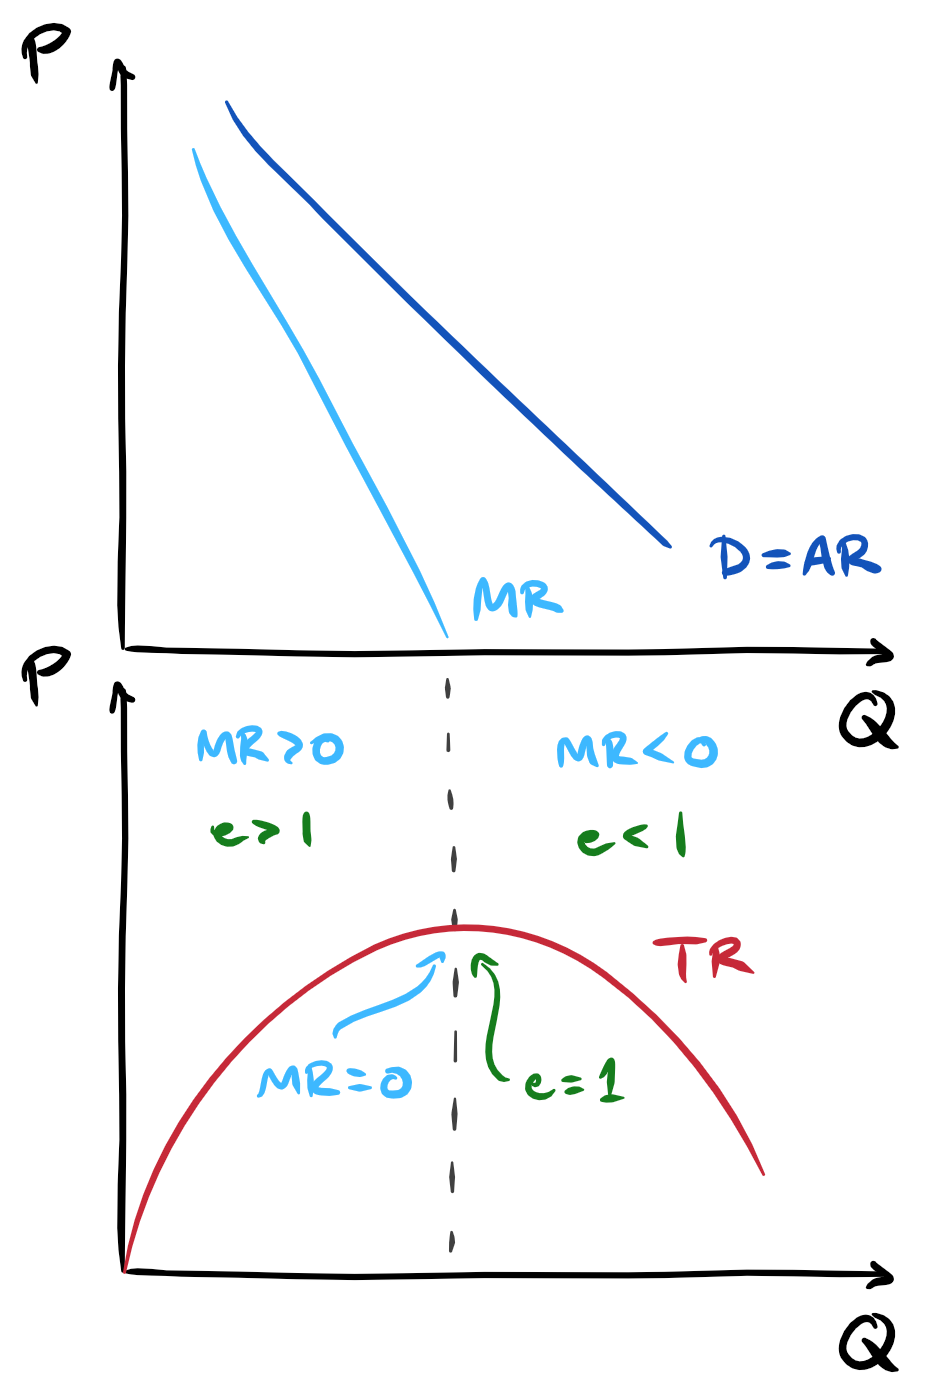
\includegraphics[width=60mm]{1193 monopolist profits.PNG}
\caption{Total, Average, and Marginal Revenue for a Monopoly}
\end{figure}


So the single-price monopolist's marginal revenue is always less than the price. It's the price \textit{minus} the revenue lost by reducing the price of all units.

\subsubsection{Short--Run Profit Maximization}

To maximize profits the firm has to 1) Shut down operations if average variable cost $AVC >$ average revenue $P$, and 2) Produce at the quantity where $MR = MC$. The size of the firms profits depends on the position of the average total cost $ATC$ curve.


\begin{figure}
\center
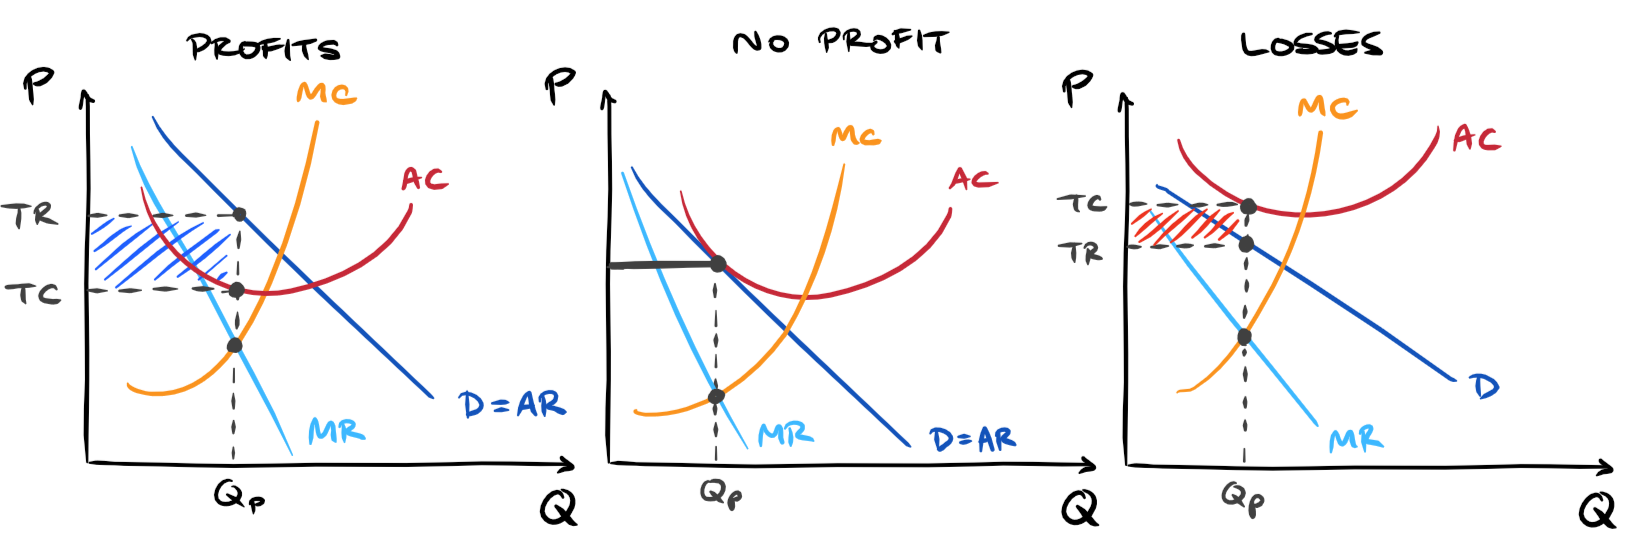
\includegraphics[width=130mm]{1202 monopolies profits losses.PNG}
\caption{Positive Profits, Normal Profits, and Losses of a Monopoly}
\end{figure}


Because the monopolist is the entire industry, the short-run equilibrium of the industry is the same as the short-run profit maximizing position of the firm. 

For a perfectly competitive market, the equilibrium price and quantity is determined by the intersection of the supply and demand curves. However, monopolists do not actually have a supply curve. This is because they're not subject to the market price. Instead they consciously choose the price and quantity combination on the demand curve to produce in order to maximize profits. 

Typically this means monopolists do not produce the quantity that would be produced in a perfectly competitive market. They produce a lower quantity at a higher price. This is profitable for them, but is inefficient for society because it creates a deadweight social loss. If they produced at the perfect competition quantity there would be more economic surplus for society.

\begin{figure}
\center
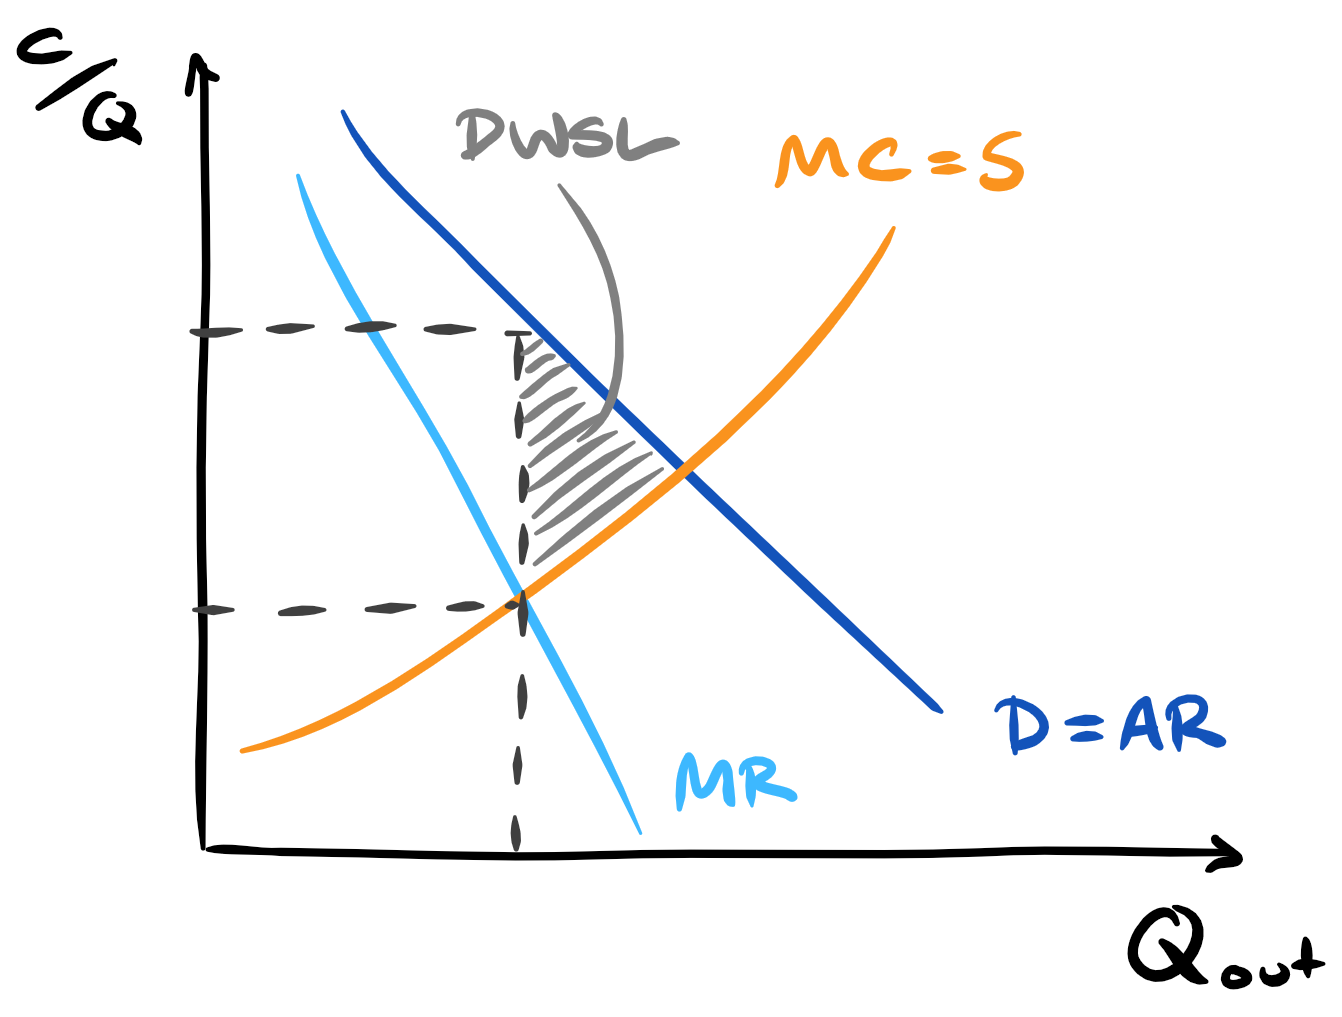
\includegraphics[width=80mm]{1210 dwsl.PNG}
\caption{Deadweight Social Loss of a Monopoly}
\end{figure}



\subsubsection{Entry Barriers and Long-Run Equilibrium}

When monopolists are making profits, that's a signal to other firms to try to enter the industry. If the monopolist is to retain its position, there must be entry barriers. 

Natural entry barriers exist when there are steep economies of scale or large setup costs. If there exists a large and already established firm, they are able to exploit economies of scale in such a way that new, smaller firms cannot compete with. Alternatively, if the costs to start up a competing firm and build rivaling infrastructure are insurmountable, as is the case with BC Hydro, smaller firms cannot compete. In these cases, a natural monopoly is said to exist.

Created entry barriers are usually established and enforced by governments. These include patent laws, which entitle patent holders to be the sole producer of a product, or government-sanctioned monopolies like Canada Post, or professional organizations that restrict the number of seats for accredited program. Barriers can also be implemented by existing firms, such as price cutting -- the practice of incurring losses that are unsustainable for the new entrant.

\subsubsection{Very Long Run and Creative Destruction}

Eventually, most of a monopoly's barriers to entry end up circumvented by innovators and the monopoly is broken. This is called created destruction. New firms develop new processes to circumvent patents, firms produce alternative products that satisfy the same needs, or firms circumvent natural monopoly barriers by producing low cost technological alternatives. For instance, cell phones have circumvented the monopoly of land-lines industries without the need to create massive infrastructure to support them.

The idea here is that monopolies that aren't propped up by government rarely persist in the long run. Further, the existence of monopolies acts as a major incentive for economic growth and innovation. 

\subsection{Cartels as Monopolies}

A cartel is when many firms decide to cooperate in order to maximize profits. Like a monopolist they choose to reduce output in order to increase the price to a monopoly level from a competitive equilibrium level.

One of the obstacles cartels face is that there are "cheaters" in the cartel who will ignore the restrictions to reduce their output. Instead they will increase their output and sell additional product at the monopoly level prices and reap the benefits. This may cause the other firms in the cartel to do the same and then the price will drop back to perfectly competitive levels. 

The other obstacle is that firms outside of the cartel will become increasingly competitive. They can find it profitable to sell additional output at equilibrium prices and may undermine the cartel. Successful cartels are often able to prevent new entries, for instance, professional industries for doctors and lawyers may limit the number of licenses to practice to keep the number of new entries down. Additionally quotas can be implemented by government to restrict the number of taxis or liquor stores. 

\subsection{Price Discriminating Monopolies}

It is profitable for a monopolist to sell different units of the same product at different prices when it gets the opportunity. Price discrimination is when a firm sells the same product at different prices \textit{for reasons not relating to differences in costs}. For instance, if you buy in bulk or buy off-season, these price differences aren't price discrimination because they could be the result of different transportation or retail costs. However, BC Hydro selling electricity at different prices for households vs. business is price discrimination. Or airplanes charging different rates depending on how long your stay is. 

As discussed in the section on Single-Price Monopolies, in order to sell additional product the monopolist has to decrease the price of all units. This results in some consumer surplus, because some consumers value the good at a higher price than it is being sold for. Price discrimination is a measure for firms to regain some of that consumer surplus. 

Price discrimination requires 1) the firm to have market power, 2) the firm to be able to distinguish between groups of consumers who may value the product differently, 3) the firm must be able to prevent arbitrage, that is, those who can buy the good at its low price re-selling it at the high-price. 

\subsubsection{Types of Price Discrimination}

There are two forms of price discrimination, that among units of output, and that among market segments. 

Price discrimination among units of output occurs when, for instance, you get a loyalty card from McDonald's and you get every eighth coffee for free. 

Price discrimination among market segments occurs when firms can distinguish between different groups' different willingness to pay for a good. For instance, senior citizens and students are given discounts because they have less disposable income and are less likely to buy the product at the rate of other members of society. The point here is that the firm will always charge the higher price to the market segment with the more inelastic demand. 

Note here that price discrimination is easier for service, like movie tickets than for goods like books. People with a different price due to price discrimination, like senior citizens, cannot purchase a whole bunch of movie tickets at a discount and sell them to teenagers at a profit. However, this is easier to do with goods, and for this reason firms place quantity limits on goods with price discriminatory schemes. 

It can be challenging for firms to distinguish between groups and assess the value placed on their product by these groups. To solve this, firms employ hurdle pricing. Hurdle pricing gets the consumers to assign themselves to categories for you. For instance, when a new book is published, its initial price is quite high. This is because the group of people who are impatient to read it are willing to pay more. After waiting some time (time is the hurdle in this case) the price decreases and other more patient consumers may buy the book for cheaper. Another example is coupons -- some people cannot be bothered with coupons and are willing to pay a higher price for goods, other people are motivated to use the coupons (jump over the hurdle) and get the good at a lower price. This is nice for the firm because they get consumers to segment themselves. 

\subsubsection{Consequences of Price Discrimination}

Firms with a negative demand curve are able to increase their profits by price discriminating, because they retrieve some of that consumer surplus for themselves. In exchange, price discriminating monopolists will produce more output than single-price monopolists. This is because when single-price monopolists produce more it depresses the price of their product. However, price discrimination negates this disincentive for price discriminating monopolists. 

This means that although some consumers are somewhat harmed because their consumer surplus is diminished, the price discriminating monopolist produces more and so society gets more total additional economic surplus. The net outcomes then is a more efficient market. Additionally, price discrimination does not have general net negative or net positive impact on consumers, because some consumers are better off while other consumers are worse off.

\section{Imperfect Competition and Game Theory}

So far we know that under perfect competition, firms are price-takers (price equals marginal cost), and under monopoly, firms are price-setters (price is above marginal cost). We're going to talk about two market structures that fall in between \textit{monopolistic competition} and \textit{oligopoly}.

Monopolistic competition is similar to perfect competition in that there is a large number of small firms. However in monopolistic competition, these small firms have some influence over price, ie. some degree of market power, such as restaurants, barbers, and grocery stores. Oligopoly describes the structure in which there are a small number of large firms, such as banks, cars, or insurance providers. 

A measure of the market power of imperfectly competitive structures is often done with \textit{industrial concentration ratio}. Typically, this is the percentage of the market share controlled by the top four largest firms $CR_4$. The higher the concentration ratio, the higher the market power. In Canada as specified by the Competition Act, the threshold for market power is $CR_4 = 65\%$.

The main difficulty with the concentration ratio is defining the relative market. For instance, if a market has five firms each with 25\% of the market share, all competing with each other, the concentration ratio would be 100\%. However, if another market had one firm controlling 60\% of the market, with 40 other firms controlling only 1\% of the market, the concentration ratio would be 63\%. However, in the first case, despite there being a larger concentration ratio, the market is much more competitive because the firms have similar market shares. Whereas in the second case, despite there being a lower concentration ratio, there is a market leader and the rest are likely to follow what the leader does.

Another problem is defining the scope of the market. For instance, whether to look at the market of potato chips in isolation, or whether to look at the market for snack foods in general. 

\subsection{Characteristics of Imperfect Competition}

\subsubsection{Product Differentiation}

Unlike a perfectly competitive market, producers are not selling a homogeneous product in the eyes of the consumer. Firms in imperfectly competitive markets sell \textit{differentiated products}, that is, products that belongs to same group of commodities but are different enough that they can be sold at different prices. These goods are substitutes, but not perfect substitutes. This is most obvious with excessive branding and advertising.

\subsubsection{Sticky Prices}

Prices are also not set by the intersection of the demand and supply curves, rather the firms fix their prices then let demand determine their sales. In perfect competition prices change continuously in response to changes in demand, however in imperfect competition firms keep their prices fixed and respond to changes in demand by modifying the level of output. Since the advent of the internet however it has become easier for firms to change prices continuously.

\subsubsection{Non-Price Competition}

Rather than competing purely with prices, firms may choose to compete with advertising, branding, quality, guarantees, services, warranties, and so-on. They do this to gain market share and also hinder the entry of new firms. This is called non-price competition, but Dr. Gateman's view that all of these things still cost money, so it is still a form price competition, perhaps better called hidden-price competition. 

\subsection{Monopolistic Competition}


Monopolistic competition is defined by the following four characteristics

\begin{enumerate}

\item Each firm has a differentiated product. So each firm has a negatively sloped demand curve, however it is still highly elastic due to close substitutes.

\item All firms have access to the same technology, and so have the same cost curves

\item There are many firms in the market. This means each firms actions do not affect each others', so they can do as they want without concerning themselves with the other firm's reactions  -- \textit{non-strategic behaviour} 

\item There is freedom of entry and exit in the industry.

\end{enumerate}

You may note here that product differentiation is the only thing that distinguishes monopolistic competition from perfect competition.

Firms in imperfectly competitive markets do not produce identical goods and spend a lot of resources on brand names and advertising, which gives the firms a small degree of market power. This market power is however limited in both the short and long runs. 

The short-run limitation on market power is the result of elasticity of demand, caused by substitutes by competing firms. In the short-run, firms resemble a monopoly. They have a negatively sloped demand curve, and maximize profits by producing the output at which $MC = MR$. 

\begin{figure}
\center
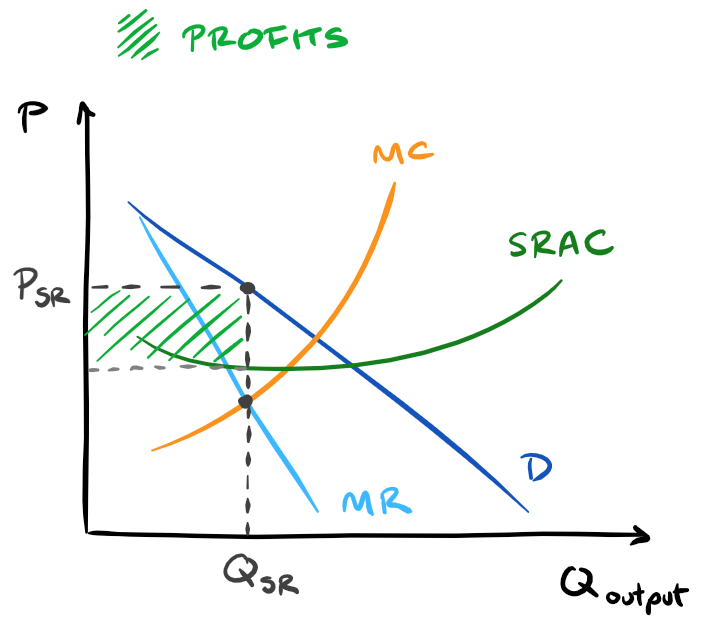
\includegraphics[width=80mm]{11-2 imperfect profits.PNG}
\caption{Long-Run Positive Profits of a Firm in Monopolistic Competition}
\end{figure}


The long-run limitation on market power comes from the free entry into the industry, which means firms will enter the industry until profits are reduced to only normal profits. This reduces the market share of each firm, so a firm's demand curve will shift left until the curve is tangent to the LRAC curve. Each firm is still maximizing profits, but those profits are now zero. 

\begin{figure}
\center
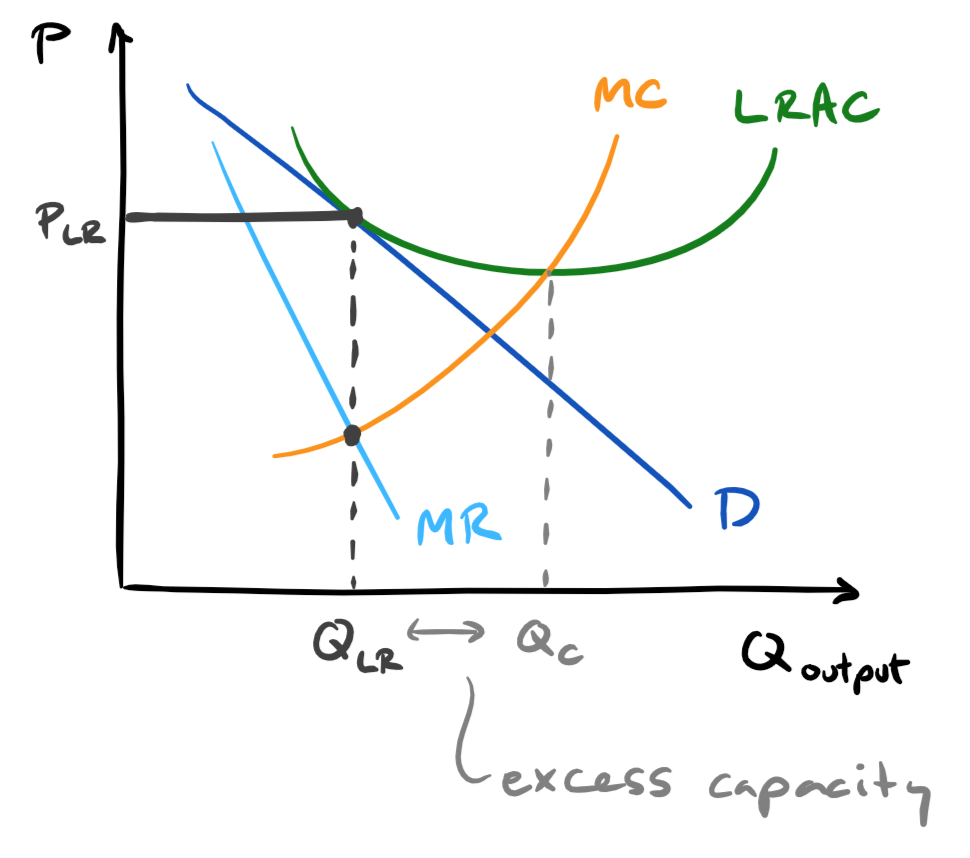
\includegraphics[width=80mm]{11-2 imperfect normmal profits.PNG}
\caption{Long-Run Normal Profits of a Firm in Monopolistic Competition}
\end{figure}


Note that in the long-run, a firm in imperfect competition is producing at a quantity less than the quantity at which the LRAC is at its minimum. In other words, they are operating at \textit{excess capacity}. The firm could reduce its costs by increasing their output, but that would mean they stop maximizing profits because they would no longer be operating at the quantity at which $MR = MC$.

This seems to be very inefficient because many industries are in monopolistic competition, so many industries are not minimizing costs/prices. However economists argue that this gives rise to a variety of brands, which may have more societal value than lower prices. So there is a trade-off between diversity of tastes and lower prices.


\subsection{Oligopoly}

In an oligopoly there are a small number of large firms and there is a high concentration ratio. Entry and exit to the industry is difficult but not impossible, often because barriers to entry associated with high start-up costs and the established firms exploiting economies of scale. 

Profit maximization is challenging for an oligopoly. Like other market structures, this is achieved by equating marginal cost and marginal revenue, however, for an oligopolist marginal revenue depends on the behaviour of its competitors. Because oligopolists must consider their competitors responses to their action, they exhibit \textit{strategic behaviour}. 

The oligopoly faces a dilemma very similar to that of cartels. The firms could cooperate (collude) to maximize their joint profits by restricting output. However, this leaves an opportunity for firms to improve their individual profits by cheating, which forces everyone to cheat so everyone makes less profit than if they cooperated -- ie. the prisoner's dilemma.


For this reason, and others, we can analyze the strategic behaviour of firms using \textit{game theory}, the study of decision making in situations in which one player anticipates the reactions of other players to its own actions.

\subsection{Game Theory (Strategic Behaviour)}

Let's first take a look at the basic dilemma of oligopoly as described above. The options and outcomes can be described in the following payoff matrix. 

\begin{figure}
\center
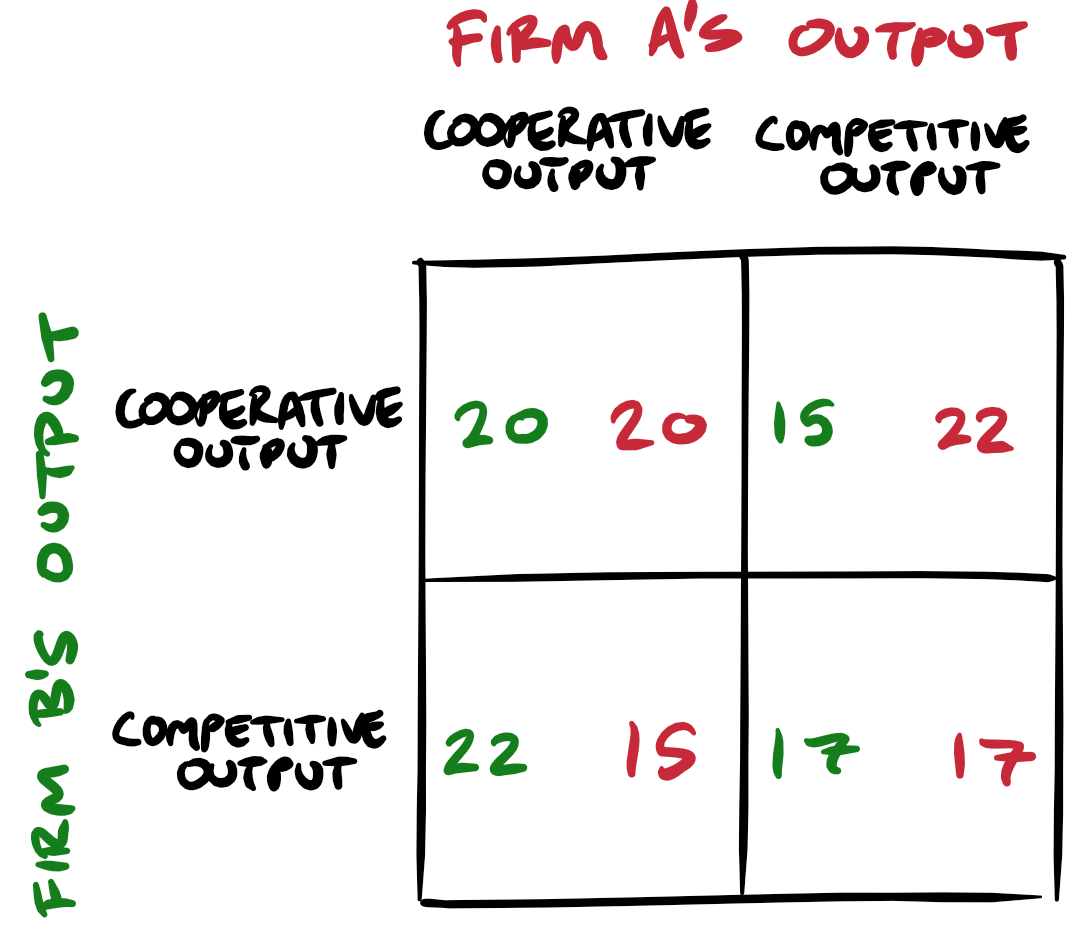
\includegraphics[width=80mm]{11-3 payoff matrix.PNG}
\caption{Oligopoly Dilemma Payoff Matrix}
\end{figure}

Cooperation would result in the highest overall level of profit, but leaves each firm with an incentive to cheat. For this reason, unless the cooperative outcome can be enforced, the cooperative outcome is unstable -- not in equilibrium. 

Assume the firms know that the cooperative outcome cannot be enforced and thus is impossible in the long term. Both firms will access their best option for both scenarios as follows: If the other firm produces at the cooperative output, then I can maximize my profits by producing at above the cooperative output. Additionally, if the other firm produces at above the cooperative output, then I can again maximize my profits by also producing at above the cooperative output. So no matter what the other firm does, I should produce above the cooperative output. This is called a \textit{dominant strategy} -- the case in which following a specific strategy yields the highest payoff regardless of what the other player does. 

So each firm ends up producing at above the cooperative output, and both make less than the potential profits they could make it they cooperated. 

\subsubsection{Nash Equilibrium}

The \textit{Nash equilibrium} is the situation described above in which both firms are producing above the cooperative output despite it not being the overall best option. It is the situation in which both players has no incentive to change their strategy given the strategy of the other player. 

When each player has a dominant strategy, it will result in a Nash equilibrium. In the case above, if either player changes their strategy, they will lose profits. So the Nash equilibrium is the situation that will arise when people make rational decisions in the absence of cooperation. Importantly, it is self-policing, that is, there no no need for someone to enforce it. 

You are said to be in a situation of \textit{Pareto optimum} when you cannot make someone better off without making someone else worse off. 

Let's look at some examples of non-sequential game situations.

\begin{figure}
\center
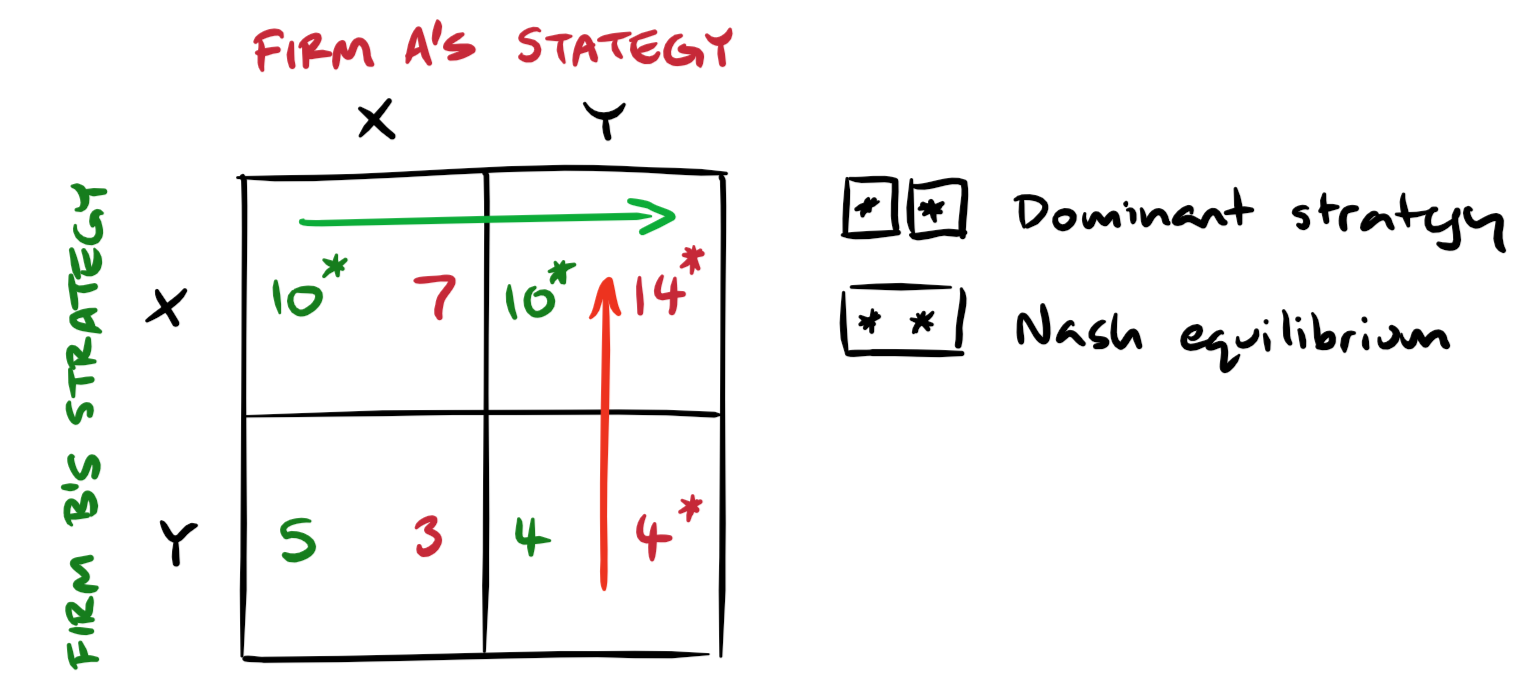
\includegraphics[width=80mm]{11-20 both dominant.PNG}
\caption{Nash Equilibrium, Two Dominant Strategies}
\end{figure}

In this situation, both players have a dominant strategy. Which result in a Nash equilibrium (two stars) and a Pareto optimum because neither player can improve their conditions.

\begin{figure}
\center
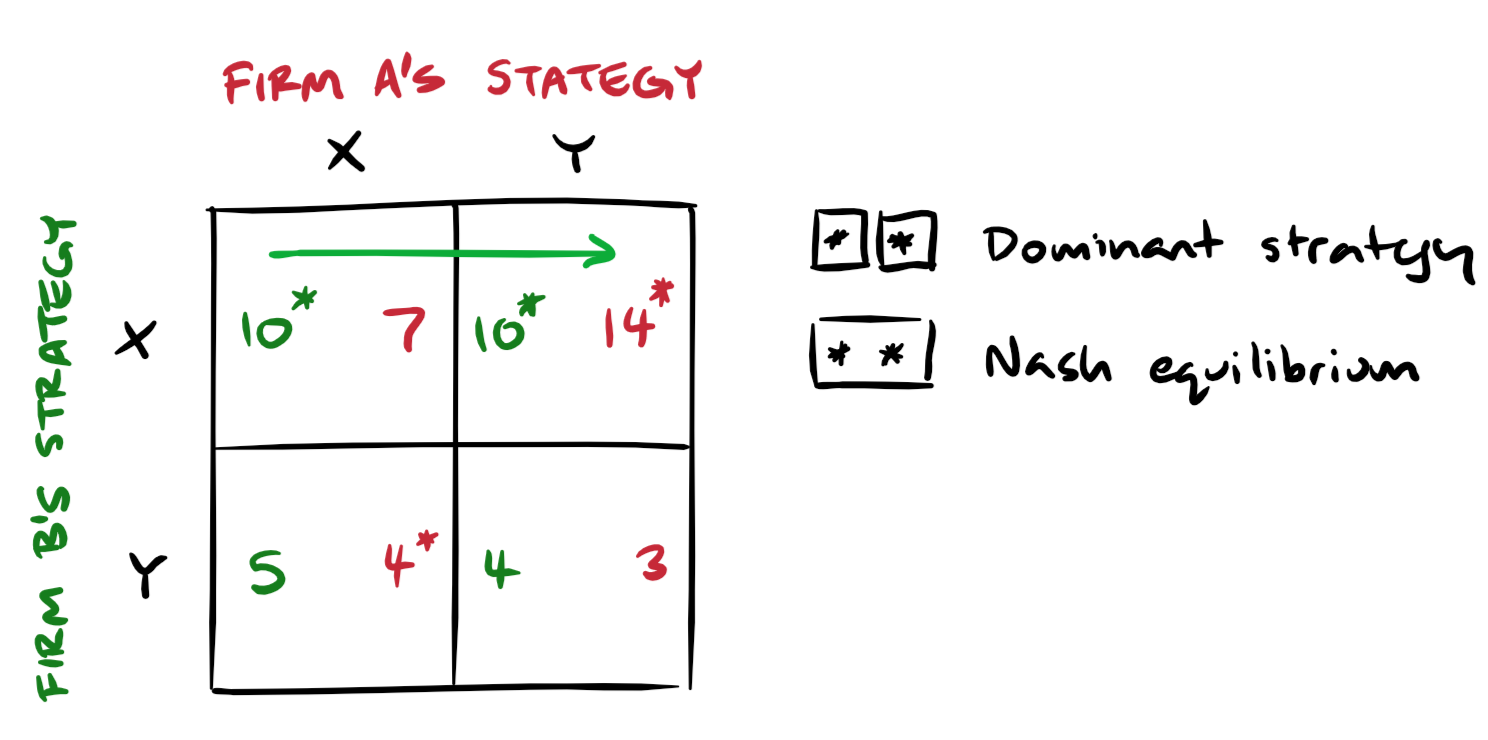
\includegraphics[width=80mm]{11-21 one dominant.PNG}
\caption{Nash Equilibrium, One Dominant Strategy}
\end{figure}


In this situation, only one player has a dominant strategy, but will still result in a Nash equilibrium and a Pareto optimum. 

\begin{figure}
\center
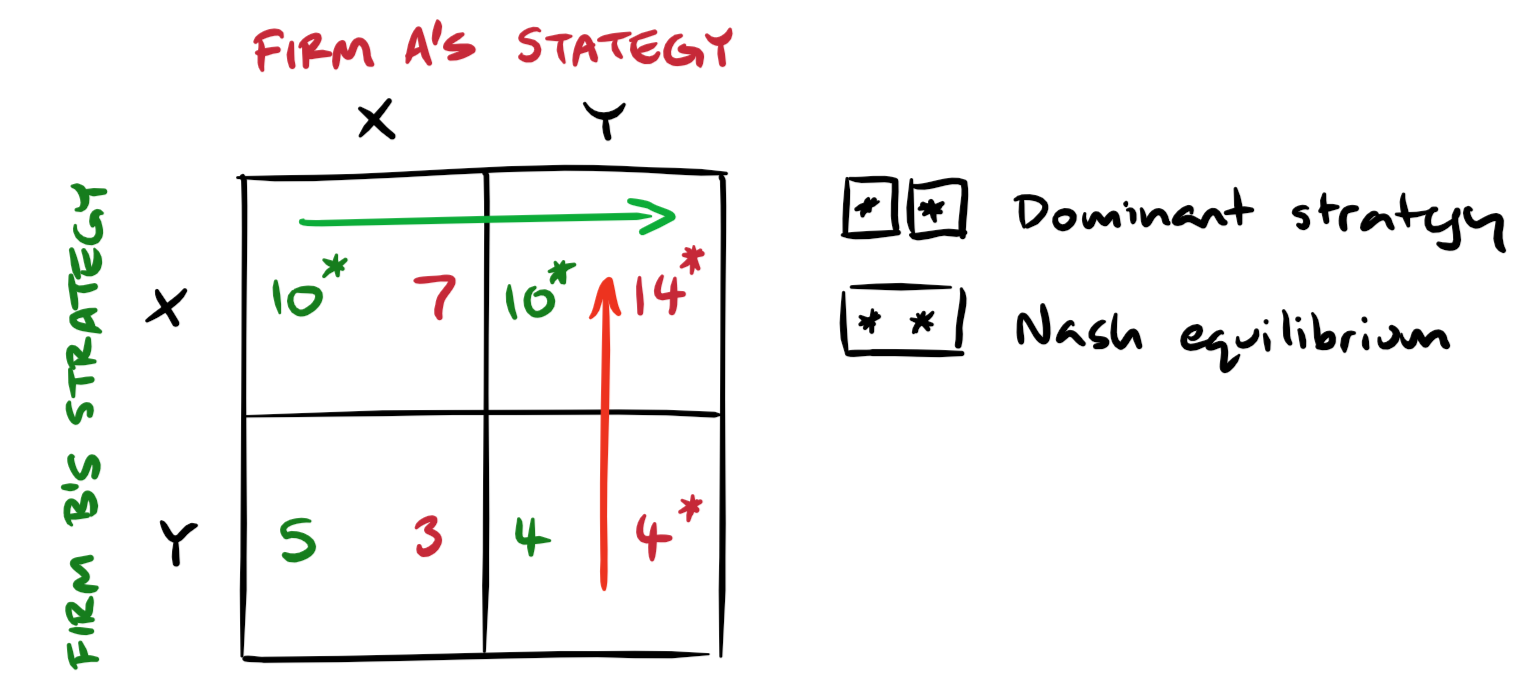
\includegraphics[width=80mm]{11-20 both dominant.PNG}
\caption{Nash Equilibrium, No Dominant Strategies}
\end{figure}

In this situation, neither player has a dominant strategy. This results in two separate Nash equilibriums. This situation also results in a Pareto optimum. Before the Pareto optimum was obvious because neither player could improve their conditions, but in this case, it's a Pareto optimum because neither player can improve their conditions without making the other player worse off. 

\begin{figure}
\center
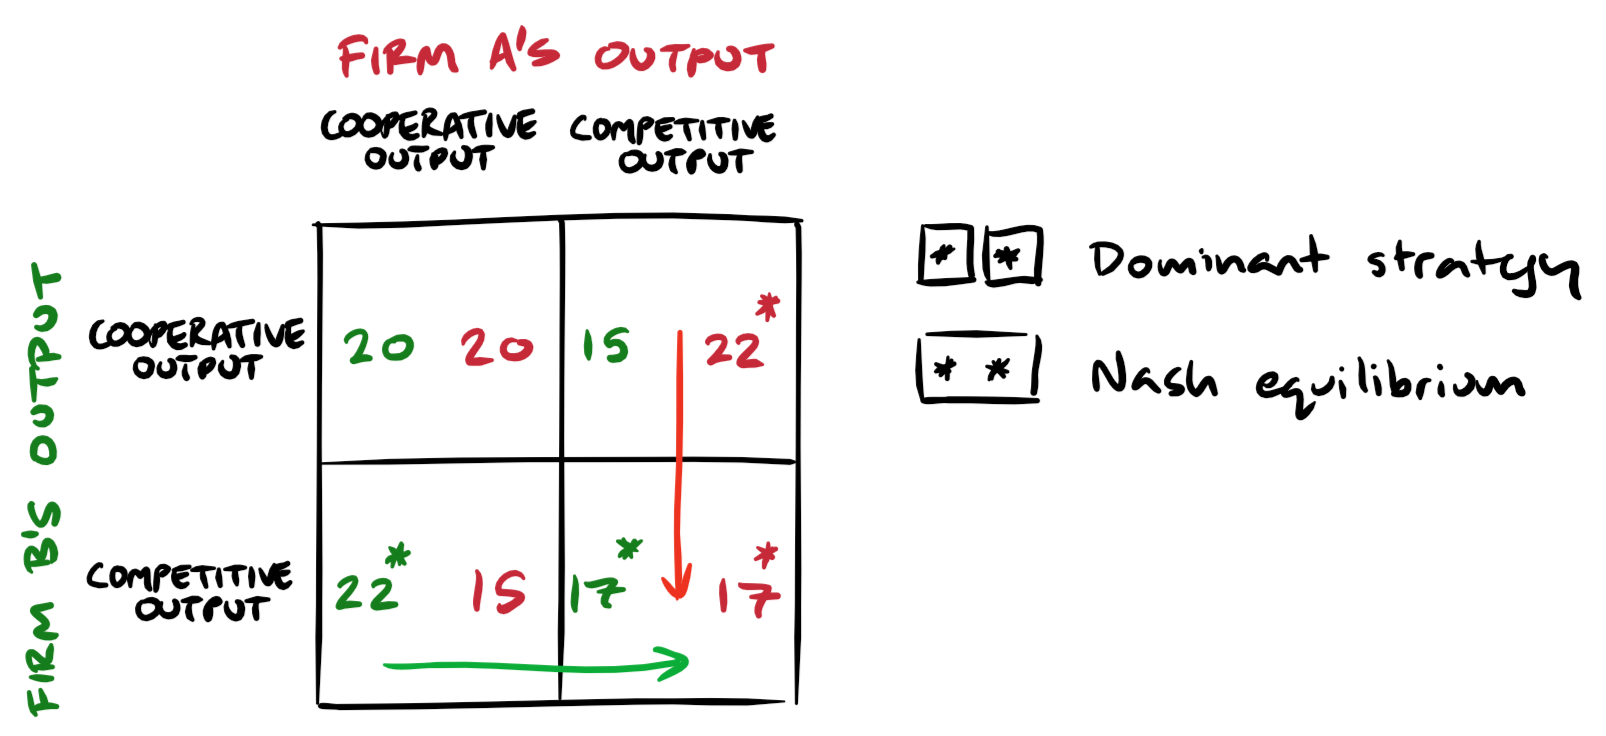
\includegraphics[width=80mm]{11-25.PNG}
\caption{Nash Equilibrium, Oligopoly Dilemma}
\end{figure}


This final situation is the same as the prisoner's dilemma discussed above. Both players have a dominant strategy which results in a Nash equilibrium. However, this situation is not a Pareto optimum, because they could both increase their conditions without harming the other player if they chose to cooperate. 

This highlights the conflict between the self-interest of the individual and the broader interests of the group. 

In these cases we have to assume that each player has full knowledge of the outcomes, and is motivated by self-interest. 

\subsection{Oligopoly in Practice}

Firms can either agree to collude explicitly -- which is illegal if discovered, or collude tactically  -- which is a recognition of common interests without an explicit agreement. 

Even if there is collusion to agree on output restrictions, oligopolies will still compete for market share by advertising or offering secret discounts, or compete by innovating. 

Barriers to entry are an important part of oligopoly. Without significant barriers to entry, firms will enter and decrease the profits of existing firms. There can be natural barriers to entry like start-up costs or economies of scale, but also be artificial barriers. Examples of artificial barriers include advertising, \textit{predatory pricing}, and \textit{brand proliferation} -- diluting the market with excessive brands owned by the same companies, so even if a new firm entered the market and beat out another brand, it would only gain a small fraction of market share. 

Some economists claim that oligopoly results in more innovation than occurs in other market structures. Oligopolists are highly motivated to innovate because they face strong competition from rivals (unlike monopolists), and can expect to keep significant shares of the profits earned through innovation. 

Oligopolies are a common market structure because of industries where the minimum efficient scale is too high to support new firms. Public policy should be focused on keeping oligopolists competing rather than colluding, and keeping their focus on innovating products and reducing costs, rather than erecting entry barriers.

\section{Efficiency and Public Policy}

Let's now discuss the efficiency of these different market structures, and see why people like certain structures and dislike other structures.

First lets review some criteria of these market structures. 


\begin{table}[ht]
  \centering
  \caption{Review of Market Structures}
  \begin{tabular}{
  		>{}m{0.75in} 
  		>{}m{0.85in} 
  		>{}m{0.7in} 
  		>{}m{0.9in}
  		>{}m{01in}  		  		
  		}
    \toprule
    \textbf{Criteria} & \textbf{Monopoly} & \textbf{Oligopoly} & \textbf{Monopolistic Competition} & \textbf{Perfect  Competition}  \\ 
    \midrule
	\textbf{Market Power} & Complete & Lots & Some & None \\
	\textbf{\# Firms} & One  & Several  & Many  & Very Many  \\
	\textbf{Good} & Unique & Similar & Differentiated & Homogeneous \\
	\textbf{Entry/Exit} & Impossible & Difficult & Easy & Free \\
	\textbf{LR Profits} & Yes & Yes & No & No \\
	\textbf{Prices} & Sets $P>MC$ & $P>MC$ & Sets $P>MC$ & Takes $P=MC$ \\

	\bottomrule

  \end{tabular}
\end{table}


Efficiency requires that factors of production are fully employed, and that no resources are wasted. This applies to both individuals/firms and greater society. There are two different kinds of efficiency, however, \textit{Productive Efficiency} and \textit{Allocative Efficiency}. 

\subsection{Productive Efficiency}

Productive efficiency is pretty straightforward, it means that you get the most output for the least input. However, there are two types of productive efficiency, that of the firm and that of the industry. 

Productive efficiency for the firm requires that the firm produces at the least possible cost (lowest point of the LRAC). 

Productive efficiency for the industry requires that the entire output of the industry is produced at the least possible cost. For instance, if firm A is producing cheese wheels at \$5/unit but firm B is producing cheese wheels at \$1/unit, then the industry isn't being productively efficient, because if firm B was producing for firm A, then society would have \$4 to produce something else with. 

In other words, each firm must have the same marginal cost, $MC_A = MC_B$. If the economy is not being productively efficient on the firm and industry levels, it will not be at the edge of the PPC. Any point on the PPB is productively efficient.

\subsection{Allocative Efficiency}

This considers how much value people are getting from goods relative to each other. For instance, if a producer could make either beer or pizza, but decided to produce so much beer that people were hammered and their marginal utility was diminishing, but did not produce any pizza even though people were really hungry, then the economy would not be allocatively efficient. 

To be allocatively efficient, the marginal cost of production must equal the price of each good produced. Consumers face the market price of some good, they will adjust them consumption until the marginal value is equal to the price, so in other words marginal value to consumers must equal marginal cost to producers, $P = MV = MC$.  Basically this just means producers aren't selling to you at a ripoff price.

Note, that different to productive efficiency, only one point on the PPC curve is allocatively efficient, and a society cannot be allocatively efficient without being productively efficient. That means there is only one point at which society is being most efficient, the point where $P = MC$. 

\subsection{Efficiency of Market Structures}

\subsubsection{Perfect Competition}

In the long-run, perfect competitors produce at their lowest costs, so both firms and industries they are productively efficient. Perfect competitors also equate marginal cost to price, so perfectly competitor market would also be allocatively efficient. 

\subsubsection{Monopoly}

A monopolist, like perfect competitors, will find itself producing at its lowest costs to maximize profits, so they are also productively efficient. Since they also represent the industry, it follows the industry is also productively efficient. 

However, monopolists choose prices that are greater than marginal cost, so monopolies are not allocatively efficient. 

\subsubsection{Monopolistic Competition and Oligopoly}

Monopolists and oligopolists have incentive to maximize their profits, so firms will typically be productively efficient. However, we cannot say whether the entire industry will be productively efficient. Because these producers have differentiated products, there is no one standard price or cost, so we can't say for certain whether marginal costs are the same for everyone.

Typically, because they have downward sloping demand curves, price usually exceeds marginal cost, so monopolistic competition and oligopoly are not allocatively efficient. However, they still are better than monopolies.

\subsection{Consumer and Producer Surplus}

Recall that consumer surplus is when the consumer is paying less than what he values the product for, and that producer surplus is when the producer is selling the product for more than they value the product for (how much it cost to make). 

Total surplus is only maximized at the equilibrium price/quantity, where the market is allocatively efficient. 

With a monopoly, the monopolist sets the quantity below the equilibrium quantity so they can sell the product at a higher price. This means they can capture some of the consumer surplus, however society loses overall surplus and is therefore not allocatively efficient.

\subsection{Economic Regulation to Promote Efficiency}

One of the main goals of government public policy is to promote the allocative efficiency of the market. The major way to do this is to encourage competition and discourage monopolies. In Canada, this is called competition policy, in the US this is called anti-trust policy. 

\subsubsection{Regulation of Natural Monopolies}

With a natural monopoly, economies of scale and start-up costs are so dominant that there is only room enough for one firm to operate competitively. For instance, assume that 100 people demand electricity, and the minimum efficient scale for electricity providers is 100. Then there is only room for one firm. 

Governments either respond to natural monopolies by assuming public ownership of them, or by allowing private ownership but regulating it. Either way, the government must impose a pricing policy to prevent prices rising to monopoly prices. There are three general strategies. 

\begin{enumerate}

\item \textbf{Marginal-Cost Pricing} is when the price is set to the marginal cost, $P = MC$. This leads to allocative efficiency, but is not profit-maximizing, because $MC \neq MR$. So this causes tension between the regulator and the firm, and the firm can suffer losses if it isn't subsidized by the government.

\item \textbf{Average-Cost Pricing} is when prices are set just high enough to cover its expenses, $P = AC$. This means the firm is making normal profits and doesn't need to be subsidized, but it is allocatively inefficient because $P \neq MC$. Additionally, the firm has little incentive to expand capacity and decrease costs, so over time it's not productively efficient.

\item \textbf{Rate of Return Regulation} is when the government stops regulating the price, but rather regulates the firms profits. They will allow profit rates for something deemed reasonable like 5\% on-top of average cost.

\end{enumerate}

%img 12-7 in book and 12-19 gbook, pricing for different strategies%

As an aside, governments will not always prevent monopolies. In section 96 of the Competition act, there is an exception for if the firms can show that by merging, they can become more efficient or exploit economies of scale and reduce their LRAC. If these cost savings are such that the price can be decreased for the consumer so much that these savings offset the possible price increase due to monopoly, then the government will not block the merge. 

\subsubsection{Regulation of Oligopolies}

Policy makers have become increasingly skeptical that oligopolies can or should be regulated by governments for a variety of reasons. One such reason is that oligopolies are an excellent source of innovation. Another reason is that there has been a bad record of regulators becoming sympathetic to the industry they were suppose to be regulating, and often sought to reduce rather than increase competition. 

Interestingly, due to globalization and the rise of information technology, local industries that may have had little competition previously are now exposed to more widespread competition. 


\section{Role of Government}

Governments have existed since shortly after the Neolithic Agricultural Revolution and they've stuck around since that time, so they've clearly figured out something that's working for them. Since that time, the main function is that they have maintained a monopoly on violence. The government is the only one who is allowed to kill people, kidnap people, lock people up, or deprive people of their liberty. 

For this reason, it's an easily abused power and needs lots of checks and balances as to not descend into abusive dictatorships. However, without it countries tend to descend into tribal conflicts with competing warlords. When the government is secure with its monopoly of violence and functions with restrictions on its abuse, citizens tend to be safest and happiest. Their monopoly of violence is required for economic prosperity.

\subsection{Basic Function of Government}

Adam Smith said that the first duty of governments was to protect the society from the invasion of another society, and the second duty was to protect individuals in the society from oppression from each other. Additionally, governments must define and enforce security of property. 

Rather than provide economic assistance to developing countries, assistance is increasingly taking the form of political assistance (called institution building) because without a secure government and established institutions, economic prosperity is impossible. 

\subsection{The Case for Free Markets}

\subsubsection{Allocative Efficiency}

The formal defence is based on the concept of allocative efficiency. It goes like this: If all markets were perfectly competitive and if governments allowed prices to be determined by supply and demand, then price would equal marginal cost. So then the economy would be allocatively efficient and consumer and producer surplus would be maximized. 

\subsubsection{Automatic Coordination}

Changes in consumer preferences and producer costs change the prices of goods. These price changes are signals to the industry, and the separate decisions made by countless individuals all work together to coordinate the economy without any centralized authority. The entire market can operate without someone having to understand the whole system, and responses to shortages and surpluses are made much more rapidly than if there was a group of central planners.

\subsubsection{Innovation and Growth}

Many goods and technologies that have contributed to the increase in the public quality of life were created by individuals in pursuit of profits. In a market economy, individuals risk time and money in hopes of developing products to make profits, and some succeed and many fail. This process works by trial and error and the independent motivations of individuals. 

In a centrally planned economy, planners have to guess the direction of technology. Indeed, they can achieve incredible things by devoting massive effort to a specific cause when chosen well, but they also can fail miserably. A huge failure of centrally planned economies was to encourage innovation, whereas the pursuit of profits have proven to stimulate innovation and growth. 

\subsubsection{Decentralization of Power}

Free markets tend to decentralize power. Rather than consolidating political power and economic power into one entity, they are both spread out. This diminishes the threat of bribery and corruption. Large firms/unions can exist and are powerful, but they remand constrained by competition. 

\subsection{The Case for Government Intervention}

Market failures are situations in which the free market fails to be allocatively efficiency. Note that in all market structures other than perfect competition, firms enjoy a negatively sloped demand curve. This means that they have some degree of market power, which means that price will exceed marginal cost, which means that they will never achieve complete allocative efficiency. However, there are situations of significant failures of markets to achieve allocative efficiency. 

\subsubsection{Market Power}

Market power is inevitable in many industries. Significant economies of scale allow the existence of natural monopolies. Firms selling differentiated products are given some ability to set their prices. Firms that innovate new products or processes gain temporary monopolies above other firms until other firms catch up. In any of these cases, firms gain market power (downard sloping D curve) and set their price above marginal cost, resulting in allocative inefficiency. 

\subsubsection{Externalities}

\textit{Externalities} are side-effects that impose costs or benefits on others, not considered in the transaction. They're unintended or unaccounted for consequences of transactions. There can be positive externalities (good accidental outcomes), and negative externalities (bad accidental outcomes). 

Private costs are the costs faced by the decision makers. Social costs are the total cost to society -- these include the private costs, but also include possible costs imposed on third parties. For instance, if I carve a spoon out of wood and sell it to a buyer. My private costs are the cost of the piece of wood and the cost of my time. However, if I dump the wood shavings into my neighbours yard, that's an extra cost for my neighbour. So in this case, there is a discrepancy between private costs and social cost, which means there's an externality. 

When there is a positive externality, the good is underproduced, so demand will rise. When there is a  negative externality, the good is overproduced, so demand will fall. Governments can influence these by instigating taxes or subsidies.

The presence of externalities leads to allocative inefficiency, even in a perfectly competitive market. 

\subsubsection{Non-Rivalrous and Non-Excludable Goods}

Non-rivalrous goods mean that consumption by one person doesn't diminish the consumption of another. Chocolate bars are rivalrous because if I eat the chocolate bar, someone else cannot also eat it. However, radio is non-rivalrous because if I listen to the radio, that does not in any way inhibit other people listening to the radio. 

Non-excludable goods mean that people cannot be prevented from consuming the good. The chocolate bar discussed above is excludable, because if I buy it first, you cannot have it. Similarly, the radio is non-excludable because the radio company cannot stop you from listening to the radio waves if you have a radio. These combinations give rise to four kinds of goods. 

\begin{enumerate}

	\item \textbf{Private Goods} are excludable and rivalrous, like the chocolate bar. These are pretty straight forward and cause no problems for public policy.

	\item \textbf{Club Goods} are excludable but non-rivalrous goods, called Club goods because you need to be in the "club" to get them. For instance, think of an art-gallery as a club good. You pay for entrance, but space permitting, you looking at a painting doesn't stop someone else from looking at a painting. However, if at capacity and congested, these can become rivalrous. 
	
	
	\item \textbf{Common-Property Goods} are non-excludable but rivalrous goods, like clean air or fish in the sea. There is no practical way for a free-market to get people to pay for consuming air, but there is also only so much of it to go around. This usually results in overconsumption or depletion, often called the tragedy of the commons.
		
	\item \textbf{Public Goods} are non-exculable and non-rivalrous, like streetlights or national defence or information. There's no practical way to get people to pay for using these goods, and in addition, consumption of one person does not diminish consumption by another. This tends to cause the free-rider problem, in which the good tends to be underproduced. 

\end{enumerate}

Because the market has no way of charging people for non-excludable goods, the market has no incentive to provide these goods. For this reason, markets fail for non-excludable goods and these goods tend to be provided by the government. 

\subsubsection{Asymmetric Information}

Asymmetric information occurs when the buyer and the seller have different information, meaning one member of a transaction can take advantage of the other. This tends to come in two forms, \textit{adverse selection} and \textit{moral hazard}. 

Moral hazard is when one party is protected from risk -- ie. they can shift the costs onto the other party. For instance, if a person has car  insurance, they may be more inclined to drive unsafely. If "too big to fail" banks are bailed out, they have incentive to continue to make risky lending practices. Or for instance, a dentist may lie and say that you need to keep coming in for more treatment. All of these are moral hazards. 

Adverse selection is when the seller and buyer have different relevant information when the contract is made. This tends to tilt the selection of goods to poorer quality. There are two cases 1) that in which the seller knows more -- ex. a used car dealership selling a poor quality car and passing it off as good quality, and 2) that in which the buyer knows more -- ex. a person buying insurance does not disclose the fact they they're addicted to cocaine. Adverse selection can lead to market failures because people do not trust each other, thus do not make transactions that would be beneficial to both members. 

Signaling is used to counter asymmetrical information, these include warranties, degrees, letters of reference, referrals, and so on.

\textbf{Let's quickly summarize the points of this chapter.}

\begin{enumerate}

\item Market power leads to allocative inefficiency.

\item Externalities lead to allocative inefficiency.

\item Non-excludable goods cannot be provided by markets.

\item Asymmetric information leads to allocative inefficiency.

\end{enumerate}

\subsection{Other Social Goals of Government}

Governments try to provide other goods and enforce other regulations not for economic reasons, but for social reasons. 

For instance, merit goods like health care, education, and other social services are goods provided based on their merits. 

Paternalism is the act of government intervening in individuals' free choice to enforce behaviour that is not necessarily that people want, but based on what the government believes is good for them, for instance making addictive drugs illegal and requiring the use of seatbelts. 

Social obligations are another service, for instance, you cannot pay someone to do jury duty for you and you cannot sell your vote, even though in a free economy such transactions would be desirable to some. 

All this to say is that although these things may decrease allocative efficiency, many people believe there is a tradeoff between social goals and allocative efficiency. 





% ----------------------------- %
% -------- BACK MATTER -------- %
% ----------------------------- %

% bibliography
\doublespacing
\clearpage
\bibliography{references}
\bibliographystyle{apacite} 
\pagebreak


\end{document}